\chapter{Robustness assessment}\label{chapter:robustness_assessment}

The fundamental goal of this project is to assess the suitability of posterior
agreement as a robust model selection criterion in the image classification setting.
This chapter will explore the properties of the PA kernel as a robustness metric in the
adversarial and out-of-distribution settings and will provide evidence supporting 
its suitability against baseline accuracy-based metrics.

\section{In-distribution setting}\label{sec:results_robustness}

Before addressing more relevant sources of covariate shift, an exploratory analysis
of the behavior of PA under random (noise) perturbations will be conducted. This
setting is denoted as in-distribution because a single sampling experiment is 
considered and perturbations are randomly generated, thus remaining agnostic of the
model and the learning task. \\

The first experiment will explore the behavior of the metric under different levels of 
observation mismatch following Example \ref{example:robustness}. Perfect, constant and random
classifiers will be considered under different conditions. The goal of this
experiment is to empirically assess whether the implemented PA kernel satisfies the 
properties of a robustness metric established in Proposition \ref{properties:robustness}.

\begin{experiment}
    A binary sample $\bm{y} \overset{\text{iid}}{\sim} \operatorname{Bernoulli}(p)$ of size 1000 is generated, 
    with $p = \mathbf{P}_Y(y = 1)$. The nature of the covariates is irrelevant, as the predictive outcome of each
    classifier is obtained artificially. In particular, two classification outputs $\bm{\hat{y}}^\prime, \bm{\hat{y}}^{\prime \prime}$ are 
    considered.

    \begin{itemize}
        \item For a perfect classifier, predictions are $\bm{\hat{y}}^\prime = \bm{\hat{y}}^{\prime \prime} = \bm{y}$.
        \item For a constant classifier, predictions are $\bm{\hat{y}}^\prime = \bm{\hat{y}}^{\prime \prime} = \bm{0}$.
        \item For a random classifier, predictions $\bm{\hat{y}}^\prime, \bm{\hat{y}}^{\prime \prime}$ are generated by randomly permuting $\bm{y}$, so 
        that the number of mismatched observations depends on the value of $p$. 

        % $$
        %     \bm{\hat{y}}^\prime, \bm{\hat{y}}^{\prime \prime} \sim \operatorname{Permutation}(\bm{y})
        % $$
    \end{itemize}
        
    Furthermore, several levels of prediction confidence are simulated by artificially generating the
    output of the discriminant function. In particular,

    $$
    F_{\hat{y}} = \frac{\Delta}{2}, \;\; \text{and} \;\; F_{1 - \hat{y}} = - \frac{\Delta}{2}, \text{ for } \hat{y} = \{\hat{y}',\hat{y}''\}.
    $$
    
    In this way, $\bm{F}$ discriminates the predicted and non-predicted class 
    by $\Delta \in \mathbb{R}$. 
    
    % Figure \ref{fig:logits_confidence} illustrates the generated $\bm{F}$ for the 
    % cases $\Delta = \{ 1/2, 1, 2\}$.
    
\end{experiment}

\begin{table}[H]
    \centering
    \begin{tabular}{l|cc|c}
    Classifier & $\beta^*$ & \textbf{PA} & Accuracy \\
    \midrule
    Perfect   & 12.33   & \textbf{\Minus 0.0082}  & 1.000   \\
    Constant  & 12.33   & \textbf{\Minus 0.0082}  & 0.525   \\
    Random    & 0.000   & \textbf{\Minus 693.14}  & 0.516   \\
    \bottomrule
    \end{tabular}
    \caption{
        Comparison of accuracy and PA values for the case $p = 1/2$.
    }
    \label{tab:empirical_table}
\end{table}


\begin{figure}[t]
    \centering
    \begin{subfigure}[b]{0.45\textwidth}
        \centering
        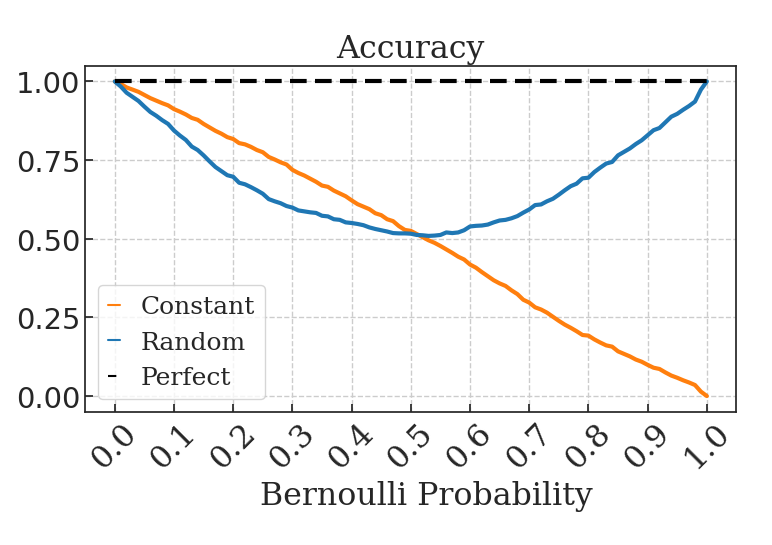
\includegraphics[width=\textwidth]{img/results_discussion/empirical/artificial_acc_final.png}
    \end{subfigure}
    \hfill
    \begin{subfigure}[b]{0.45\textwidth}
        \centering
        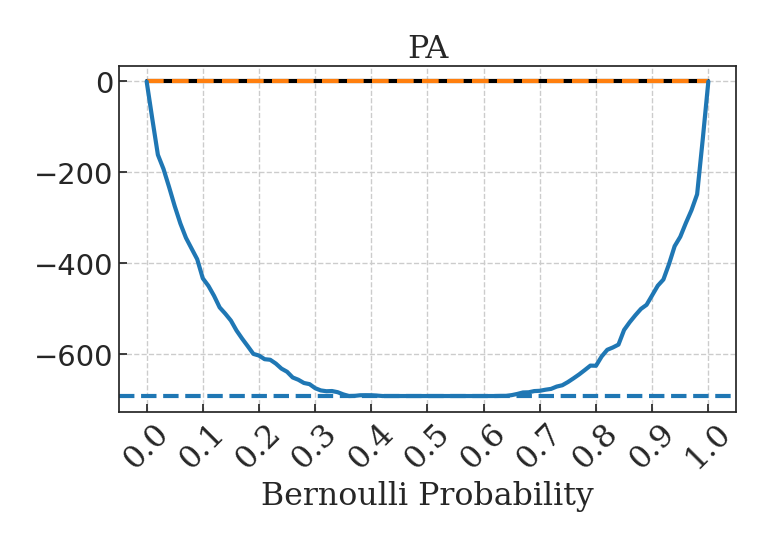
\includegraphics[width=\textwidth]{img/results_discussion/empirical/artificial_logPA_final.png}
    \end{subfigure}
    \caption{
    Evolution of PA and accuracy for constant, perfect and random classifiers across different 
    values of $p \in [0,1]$. Accuracy does not comply with the desired properties of a robustness metric
    and provides an inconsistent assessment that is exclusively driven by task performance. In contrast,
    PA continuously discriminates robust from unrobust classifiers for $p \in (0,1)$ and reaches 
    its minimum $-N \log 2$ (blue dashed line) for the random classifier when $p \in (0.3,0.7)$.
    }
    \label{fig:empirical_plot}
\end{figure}

Table \ref{tab:empirical_table} displays the values of PA and accuracy
obtained for the case $p = 1/2$. It is clear that PA is independent of the task performance
of the model, which in classification tasks is mostly reported through accuracy-based metrics, and 
instead discriminates effectively the random classifier from the rest. In particular, 
PA converges towards its minimum value $-N \log{2}$ for the random classifier 
as $\beta \longrightarrow 0$, and converges towards zero for the 
other two as $\beta \longrightarrow \infty$. This behavior aligns with the 
intuitive assessment given in Example \ref{example:robustness}, since perfect and constant 
classifiers are robust by definition, while random classifiers are extremely unrobust. \\

Figure \ref{fig:empirical_plot} extends these results across different values of 
$p \in [0,1]$. It can be observed that the lower bound, represented by the blue dashed line, 
is achieved only after a certain mismatch threshold has been reached, of approximately 
30\% of the observations. This illustrates the trade-off navigated during $\beta$ optimization, 
in which matching observations are more heavily penalized the higher the value of $\beta$ is,
whereas mismatching observations are more heavily penalized the lower the value of $\beta$ is.
A balanced random classifier (i.e. balanced on the two classes) would converge to the
lower bound for any possible original sample. \\

Finally, Figure \ref{fig:prediction_confidence} illustrates the $\beta$ optimization
process for different values of prediction confidence gap $\Delta$. The confidence gap, 
expressed as a difference in the unnormalized log-odds $\bm{F}$, is very informative with 
regard to the quality of the model, as it is intuitively expected that the latent 
space represented by a high-confidence model encodes a better set of features 
to discriminate classes than one with a lower prediction confidence. 
In particular, the optimization concerns a random classifier with $p = 1/2$ and a
sample of 100 observations, thus $\beta^{*} \longrightarrow 0$. Following the process already 
described in Section \ref{sec:pa_kernel}, we observe that
the wider is the confidence gap (i.e. the informativeness of the posterior at $\beta_0 = 1$),
the faster is the rate of convergence to the optimal value, considering that the number of
mismatching observations is the same in all cases. \\

For that reason, results presented in this work will also include situations in which both
samples are the same (i.e. $\bm{x}' = \bm{x}''$). In these cases, a pseudo-PA value will be 
obtained which will not correspond to the optimal with $\beta^{*}=0$, but will depend on the
rate with which it converges towards it. Given that convergence is faster for high confidence 
predictions, it will still be highly informative of the generalization capabilities of the model. More
specifically, models displaying a lower proportion of high-confidence observations will be 
penalized. Given that low-confidence observations are associated with wrong predictions, the 
raking of models provided by a suboptimal PA for $\bm{x}' = \bm{x}''$ will be equivalent 
to that provided by standard accuracy. Further details on the empirical behavior of the PA
metric can be found in Appendix \ref{subsec:appendix_empirical_behaviour}.

\begin{figure}[t]
    \centering
    \begin{subfigure}[b]{0.45\textwidth}
        \centering
        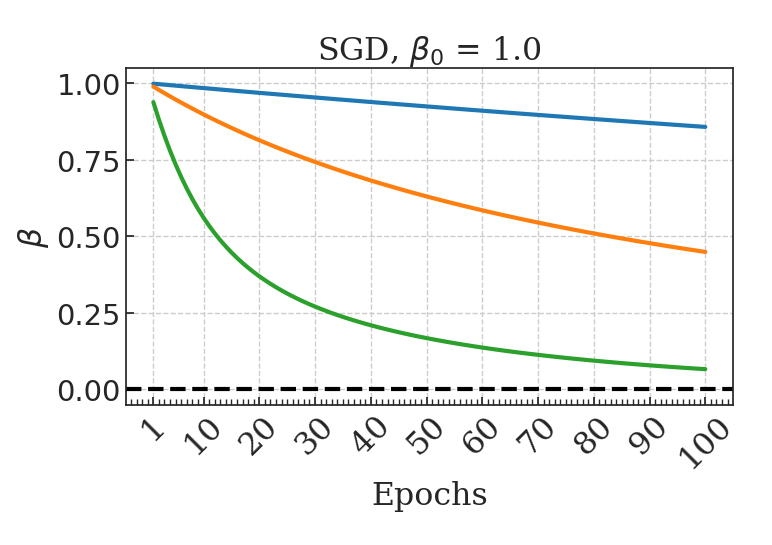
\includegraphics[width=\textwidth]{img/results_discussion/empirical/nonrob_met=betas_hue=ldiff.png}
    \end{subfigure}
    \hfill
    \begin{subfigure}[b]{0.45\textwidth}
        \centering
        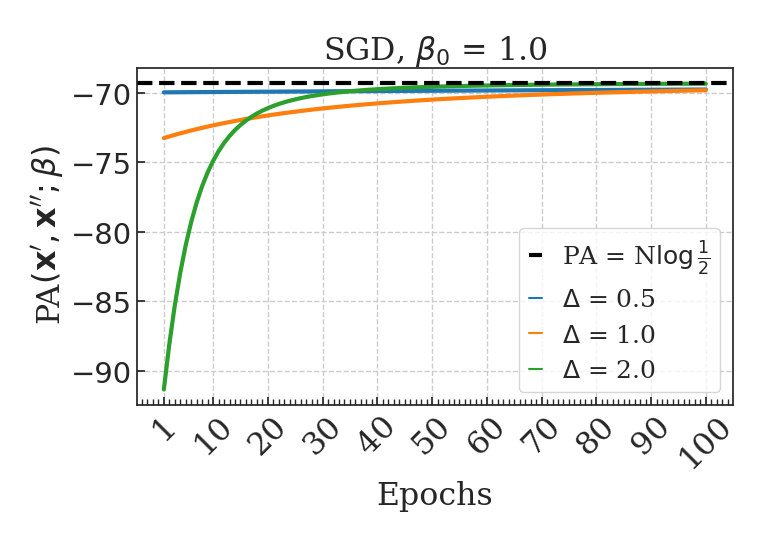
\includegraphics[width=\textwidth]{img/results_discussion/empirical/nonrob_met=logPA_hue=ldiff.png}
    \end{subfigure}
    \caption{Evolution of the PA kernel optimization under different levels of prediction 
    confidence for a random classifier with $p = 1/2$, computed over a sample of size $N=100$. 
    The rate of convergence is shown to depend on the informativeness of the posterior at $\beta_0 = 1$, and 
    consequently on the confidence gap $\Delta$. 
    An illustration of the original log-odds and 
    its associated posterior distribution can be found in Appendix \ref{subsec:appendix_empirical_behaviour}.
    }
    \label{fig:prediction_confidence}
\end{figure}

The results obtained with artificial samples motivate the exploration of more realistic
scenarios. In general, the PA metric is expected to capture the generalization capabilities
of any model yielding probabilistic predictions, regardless of the task at hand. This
already represents an incredible advantage from an epistemological perspective, as it can
be argued that the metric is agnostic of the underlying mechanism that generated the data
and even to the nature of the data itself.\\

In order to verify this claim, we will start by evaluating the robustness of two
different classifier models in two different domains under increasing levels of 
random noise. This particular setting, even if synthetically designed, is 
relevant in any classification context because it provides a general measure of the 
quality of the features learned. The presence of noise, at least 
at low levels, does not perturb the set of features that define a particular class from
a perceptual standpoint and should therefore not perturb very significantly the
predictions of robust models.

\begin{experiment}
The model under consideration is an image classifier for CIFAR10, a popular
computer vision dataset composed of colored, 32 $\times$ 32 pixel images belonging to 10
different classes \cite{krizhevskyLearningMultipleLayers}. Sample
$\bm{x}'$ contains 10.000 images and $\bm{x}''$ is generated 
by perturbing each image with white noise of increasing intensity.
A pre-trained, undefended WideResNet-28-10
\cite{BMVC2016_87}
architecture is used to evaluate the effectiveness of the attack. The 
magnitude of the perturbations is expressed in the same terms as those 
of an adversarial attack for further reference, but translate to 
using $\sigma = 3 \ell_\infty$, as 99.73\% of the
total mass of the gaussian distribution lies within the 
interval $\pm 3\sigma$.
\end{experiment}

\begin{figure}[H]
    \centering
    \begin{subfigure}[b]{0.45\textwidth}
        \centering
        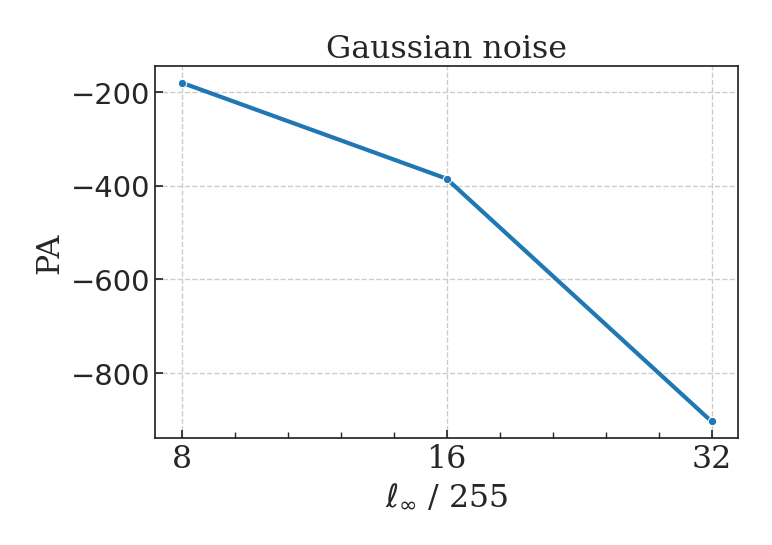
\includegraphics[width=\textwidth]{img/results_discussion/adversarial/GAUSSIAN_logPA_eps_single.png}
    \end{subfigure}
    \hfill
    \begin{subfigure}[b]{0.45\textwidth}
        \centering
        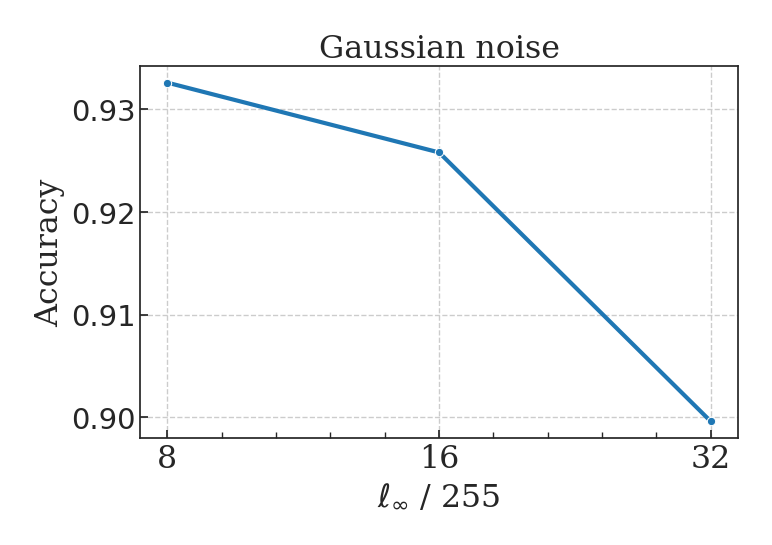
\includegraphics[width=\textwidth]{img/results_discussion/adversarial/GAUSSIAN_acc_pa_eps_single.png}
    \end{subfigure}
    \caption{PA and accuracy displayed by the CIFAR10 classifier under increasing levels of white noise. Robustness
    and task performance are shown to be non-linearly related.
    }
    \label{fig:gaussian_noise}
\end{figure}



Figure \ref{fig:gaussian_noise} shows that 
PA is highly sensitive to the presence of white noise and effectively captures the factor 
of increase in the magnitude of the perturbations. In general, gaussian perturbations genuinely simulate increasing levels of sampling randomness, as the 
perceptual features that should drive the inductive bias of the model are still present, even 
if in a proportionally dissimilar way as they were encoded. In contrast to adversarial attacks, 
these perturbations are not expected to distort the predictive outcome 
abruptly. As a result, any robustness score will be driven by the standard generalization error, including validation 
accuracy. \\

Figure \ref{fig:gaussian_optimization} expands these results by gradually adjusting
the perturbation so that it only affects a specific ratio of observations. As expected, 
$\beta \longrightarrow \infty$ in the unperturbed case, and converges
quickly to its optimal value in the rest of cases, even for a considerably large 
sample size. The decay in the PA value is less pronounced the higher
fraction of perturbed observations are there, which is consistent with the concept 
of robustness defined, as it already approaches the lower bound for these kinds of 
perturbation even when the whole sample has yet not been affected. \\


\begin{figure}[t]
    \centering
    \begin{subfigure}[b]{0.49\textwidth}
        \centering
        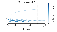
\includegraphics[width=\textwidth]{img/results_discussion/empirical/beta_100.pdf}
    \end{subfigure}
    \hfill
    \begin{subfigure}[b]{0.49\textwidth}
        \centering
        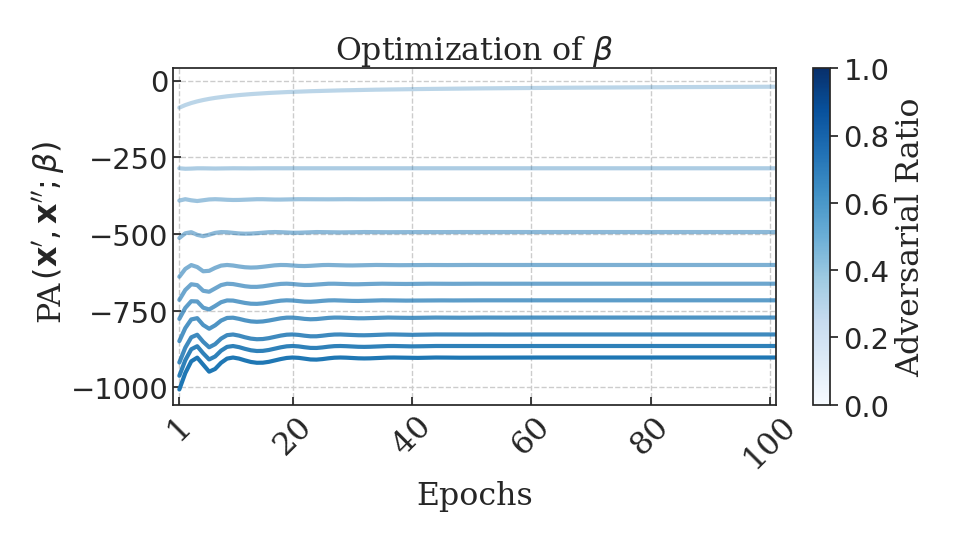
\includegraphics[width=\textwidth]{img/results_discussion/empirical/logPA_100.png}
    \end{subfigure}
    \caption{PA kernel optimization in the CIFAR10 gaussian noise setting for different ratio
    of perturbed observations. Perturbation magnitude is $\ell_\infty$ = 32 / 255.}
    \label{fig:gaussian_optimization}
\end{figure}



\begin{experiment}
The model under consideration is a sentiment classifier for IMDB,
a popular NLP dataset containing 50,000 movie reviews labeled 
as either positive or negative
\cite{maas2011learning}. 
A pre-trained DistilBERT-based architecture 
is adopted, with the appropriate tokenizer
\cite{sanh2019distilbert}. 
After a 100 epoch training using SGD with a learning rate of $10^{-3}$, the model with the highest validation
accuracy is selected. Then, the original test dataset $\bm{x}^\prime$
is incrementally perturbed to generate $\bm{x}^{\prime \prime}$, by either adding, removing or replacing 
single characters. This perturbation amounts to increasing the Levenshtein
distance $L$ between identical observations of the dataset, and the attack power
is defined as $2^{L}$.
\end{experiment}

\begin{figure}[H]
    \centering
    \begin{subfigure}[b]{0.45\textwidth}
        \centering
        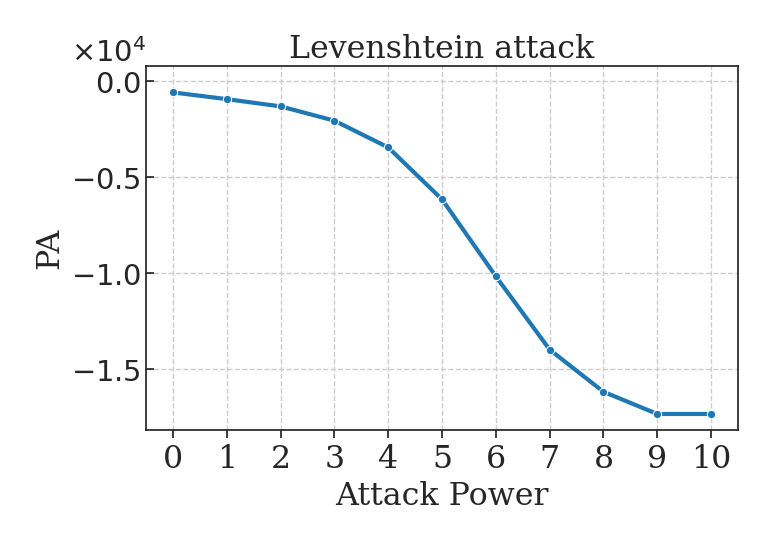
\includegraphics[width=\textwidth]{img/results_discussion/empirical/levenshtein_logPA.png}
    \end{subfigure}
    \hfill
    \begin{subfigure}[b]{0.45\textwidth}
        \centering
        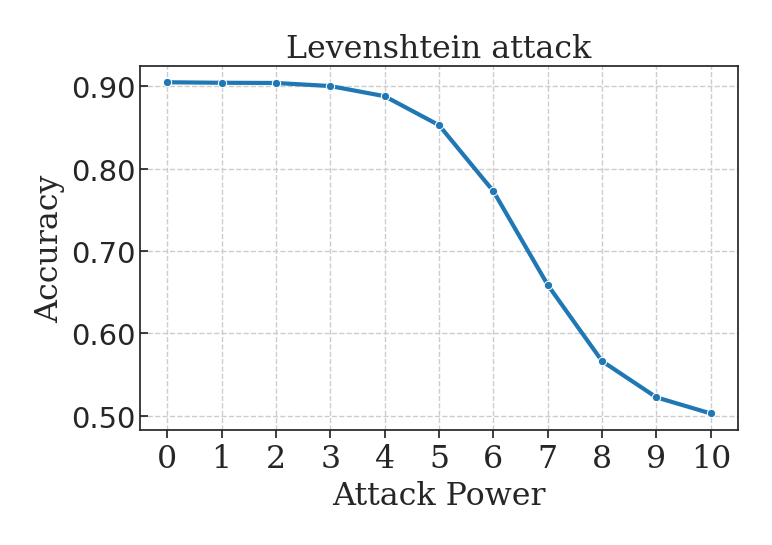
\includegraphics[width=\textwidth]{img/results_discussion/empirical/levenshtein_AFR_true.png}
    \end{subfigure}
    \caption{PA and accuracy for the IMDB sentiment classification under Levenshtein perturbations.
    The attack power is defined as $2^L$, being $L$ the Levenshtein distance between pairs of
    observations in $\bm{x}^\prime$ and $\bm{x}^{\prime\prime}$.}
    \label{fig:imdb_levenshtein}
\end{figure}

Figure \ref{fig:imdb_levenshtein} shows that PA is highly sensitive to the
presence of Levenshtein perturbations, as it is able to capture the
change in the predictive outcome of the model even when performance remains 
unaltered. In particular, accuracy remains maximum even when 4 characters
are perturbed in every observation, and begins to decrease only after that. In contrast,
PA drops significantly after the first perturbation and reaches its minimum value
after $2^9$ perturbations have been made, indicating that the outcome is maximally
unrobust. \\

Further discrepancies between accuracy and PA can be observed if the 
attack is designed to directly influence the sentiment prediction, which corresponds
to an adversarial setting. For instance, Figure \ref{fig:imdb_adversarial} shows that accuracy can be 
manipulated to increase or decrease by perturbing original observations with
adjectives that reinforce or contradict, respectively, 
the sentiment expressed in the review. In both cases, PA measures the lack of robustness in the
predictions that these perturbations represent, regardless of the task
performance displayed. The robustness against adversarial attacks in
image classification tasks will be discussed in the next section. \\

\section{Adversarial setting}\label{sec:results_adversarial}

The first real scenario in which covariate shift robustness will be measured is the
adversarial setting. This setting serves as an archetypal use case for a robustness 
metric, given that adversarial perturbations are deliberately generated to mislead the
model, and any robustness score will ultimately be driven by the effectiveness of the 
attack. In particular, PA should be highly informative about the defensive capabilities 
of models, as the posterior distribution over the hypothesis class will shift 
significantly in the presence of adversarial perturbations. This section aims to validate 
this claim and provide deeper insights into the nature of the metric. \\

It is important to note that adversarial perturbations constitute an
intermediate instance between sampling randomness and distribution shift. 
On the one hand, they emulate a sampling variation that appears 
as an outlier under the model's representation of the true class, even if
the source of variability is completely artificial. On the other
hand, samples are known to contain the set of features that should 
align with the inductive bias of the model, and so the model's ability to 
distillate those features is in question. In practice, we are evaluating the 
quality of the complex discriminator function defining a basin of stability
around original observations, and for that no deep understanding of the nature of 
the randomness of the samples or the features they encode is needed.\\

This interpretation is aligned with the measure provided by accuracy-based metrics, 
because adversarial examples do not entail any accountable source of randomness, 
but instead exploit specific vulnerabilities of models to alter the position of the 
maximum of the posterior distribution. A greater posterior overlap will still
indicate higher robustness to attacks, regardless of the nature of the model or the
attack, but optimal posteriors are expected to converge to very peaked gibbs
distributions centered at the predicted class, reducing the interpretability of PA
to that of accuracy. \\

In order to explore these claims, robustness and performance results will be
provided through the attack failure rate (AFR) value and compared to those
yielded by PA. The AFR computed with the true class labels will be used as a baseline
of model performance, whereas the AFR computed with the predicted class labels
will be a reference for robustness, as it aligns with the aforementioned
interpretation.

\begin{definition}[\emph{Attack failure rate}]
    Let $\bm{\hat{y}^\prime}, \bm{\hat{y}^{\prime\prime}} \in \mathcal{Y}^N$ be the predicted class 
    labels for $\bm{x}^\prime$ and $\bm{x}^{\prime \prime}$, respectively, 
    and let $\bm{y}\in \mathcal{Y}^N$ be the true labels. Considering the definition of accuracy
    provided in Section \ref{sec:robustness_to_covariate_shift}, the attack failure rate (AFR)
    can be expressed as

    $$
    \begin{aligned}
        \operatorname{AFR}_\text{T} &= \operatorname{Accuracy}(\bm{\hat{y}^{\prime \prime}}, \bm{y}), \\
        \operatorname{AFR}_\text{P} &= \operatorname{Accuracy}(\bm{\hat{y}^{\prime \prime}}, \bm{\hat{y}^{\prime}}).
    \end{aligned}
    $$

\end{definition}

\begin{definition}[\emph{Adversarial ratio}]
    Besides the maximum norm allowed for each perturbation, we are also interested in evaluating 
    the sensitivity of our robustness measure to the ratio of perturbed observations in the dataset, 
    also known as adversarial ratio $\alpha \in [0,1]$. The final adversarial dataset $\bm{x}''$ will be generated as

    $$
    \bm{x}'' := \alpha \bm{x}'' + (1 - \alpha) \bm{x}',
    $$

    where $\bm{x}'' = \bm{x}' + \bm{\Delta}$, as per Definition \ref{def:adversarial_perturbation}.
\end{definition}

This incremental expansion of the attack is particularly relevant for PA, as we would initially 
expect it to behave non-linearly with respect to $\alpha$ and converge faster to
the $\alpha=1$ robustness value than any accuracy-based metric, in light of the behavior observed
in Figure \ref{fig:gaussian_optimization}. \\

Before delving into the results, it is worth exploring the immediate consequences
of the previous claim, namely the fact that the maximum posterior agreement will
be achieved when gibbs distributions are highly peaked on the predicted 
class, at least for moderate attacks. This is because most adversarial 
perturbations will not succeed at misleading the model and thus drive the inverse temperature to
infinity. The divergence of $\beta^{*}$ is only limited by the set of misleading adversarial 
examples, that for being perturbed from the original class are still expected to assign a
significant confidence to the original prediction, even if not the maximum anymore.
Table \ref{tab:entropy_gibbs} illustrates this claim by showing that $\beta^{*} > 1$ 
for all robust models, resulting in a substantial decrease of the entropy between initial and 
optimal posteriors. \\

This realization allows us to break down the dataset into subsets of observations
that contribute to the final PA value in different ways, and therefore improve
the interpretation of the resulting robustness measurement.
For a start, a robust model should be expected to correctly classify most of the 
original observations with high confidence, as they
contain the features encoded in the inductive bias of the 
classifier. Original observations that do not contain these features will be misclassified,
and the lack of generalization to sampling randomness should be penalized for lowering
the confidence in the predicted class. Regarding adversarial examples, a clear
distinction between robust and non-robust models should be made based on the success 
rate of perturbations and the confidence attributed to misleading predictions. Adversarial 
perturbations on originally misclassified observations will not be of much interest,
as the effect on prediction confidence should not be as significant as in
the correctly classified ones. An interpretable expression for PA in the adversarial
setting can be obtained by approximating the optimal posterior for each of these
subsets of observations. \\

\begin{proposition}
    Let $\zeta_{\text{ERR}}$, $\zeta_{\text{MIS}}$ and $\zeta_{\text{ADV}}$ be the approximated robustness
    contributions of correctly classified original observations, misclassified original observations
    and misleading adversarial examples, respectively. Then, we can approximate PA as

    $$
    \operatorname{PA} \approx \zeta_{\text{ERR}} + \zeta_{\text{MIS}} + \zeta_{\text{ADV}} = \zeta_{\text{SAM}} + \zeta_{\text{ADV}} 
    $$

    with
    $$
    \begin{aligned}
        &\zeta_{\text{ERR}} = N \operatorname{AFR}_\text{T}^0 \operatorname{AFR}_\text{P} \log \left( 1 - 2\delta_{\text{ERR}} \right), \\
        &\zeta_{\text{MIS}} = N (1- \operatorname{AFR}_\text{T}^0) \operatorname{AFR}_\text{P} \log \left( 1 - 2\delta_{\text{MIS}} \right), \\
        &\zeta_{\text{ADV}} = N \operatorname{AFR}_\text{T}^0 (1 - \operatorname{AFR}_\text{P}) \log \delta_{\text{ADV}},
    \end{aligned}
    $$

    where $\operatorname{AFR}_\text{T}^0 \equiv \operatorname{AFR}_\text{T}(\alpha=0)$ is the accuracy of the model in the original data.
    Variables $\delta_{\text{ERR}}$, $\delta_{\text{MIS}}$ and $\delta_{\text{ADV}}$ account for the 
    average probability assigned to
    classes other than the predicted class for the three aforementioned cases 
    (see illustration in Figure \ref{fig:appendix_adv_illustration}). $\zeta_{\text{SAM}}$ aggregates
    the first two terms and will be interpreted as the sampling randomness contribution.
\end{proposition}
\begin{proof}
    See Apendix \ref{sec:appendix_results_adversarial}.
\end{proof}

Figures \ref{fig:appendix_adversarial_approx_pa_pgd} and \ref{fig:appendix_adversarial_approx_pa_fmn}
compare the true and approximated PA values under increasing adversarial ratio for
PGD and FMN attacks, respectively. It is clear that penalizations are overestimated, 
given that the average posterior probability is used and differences by defect are more 
significantly penalized than those by excess due to the nonlinear nature of the logarithm in 
the range $[0,1]$. Besides, $\beta^{*}$ is fixed to its lowest possible value (i.e. when $\alpha$ = 1),
which makes the approximation on the FMN attack less reliable for smaller adversarial 
ratio settings, as $\beta^{*}$ decreases significantly due to the effectiveness of the attack. \\

Nevertheless, the relative differences in the approximated PA values are consistent
with the true values, and the ranking of the models is largely preserved across different
$\alpha$ values. For that reason, the additional interpretability provided by this approximation
will illustrate PA expression will help characterize the source of the robust and unrobust
observed in the different models. \\

\begin{table}[t]
    \centering
        \begin{tabular}{l|rr|rr}
        Defense & $\beta^{*}_{\text{PGD}}$ & $\Delta H_{\text{PGD}}$  & $\beta^{*}_{\text{FMN}}$ & $\Delta H_{\text{FMN}}$ \\
        \midrule
        {\color{tab:orange} \textbf{Undefended}} & 0.78 & 0.048 & 0.65 & 0.10\\
        {\color{tab:blue} \textbf{Engstrom et al.}} & 15.63 & -1.204 & 2.59 & -0.71\\
        {\color{tab:green} \textbf{Athalye et al.}} & 35.48 & -3.049 & 19.84 & -2.13 \\
        {\color{tab:red} \textbf{Wong et al.}} & 15.46 & -1.229 & 4.59 & -0.96\\
        {\color{tab:purple} \textbf{Addepalli et al.}} & 15.89 & -2.023 & 6.08 & -1.71 \\
        {\color{tab:brown} \textbf{Wang et al.}} & 11.24 & -1.833 & 2.53 & -1.41\\
        \bottomrule
        \end{tabular}
        \caption{
        Entropy difference $\Delta H = H(\beta^{*}) - H(1)$
        for different models, obtained for FMN and PGD 
        $\ell_\infty$ = 8/255 attacks with $\alpha = 1$. Entropy values are 
        computed with the average posterior over correctly classified
        observations, which constitute the largest proportion of the dataset.
        Defended models converge to $\beta^{*} > 1$, whereas the undefended
        model displays $\beta^{*} < 1$. This is consistent with the interpretation
        of robustness in terms of the optimal informativeness of the posterior.
        }
        \label{tab:entropy_gibbs}
\end{table}

\begin{experiment}
The results provided in this section have been obtained using CIFAR10
\cite{krizhevskyLearningMultipleLayers},
which is widely regarded as a standard benchmark for robustness evaluation. CIFAR10 is
a balanced dataset containing 60.000 colored 32 $\times$ 32 pixel images belonging to 10
different classes. We will consider a pre-trained WideResNet-28-10
\cite{BMVC2016_87}
as a baseline, undefended model and compare it to some state-of-the-art robust ResNet50
\cite{resnet50}
models provided by the 
RobustBench \cite{croceRobustBenchStandardizedAdversarial2021a}
library under PGD \cite{madryDeepLearningModels2019}
and FMN \cite{pintorFastMinimumnormAdversarial2021}
attacks, both run for 1000 steps (see Section \ref{sec:adversarial_setting}).
The defenses applied are those proposed by 
{\color{tab:blue} \textbf{Engstrom et al.}} \cite{engstrom2019adversarial}, 
{\color{tab:green} \textbf{Athalye et al.}} \cite{AthalyeC018}, 
{\color{tab:red} \textbf{Wong et al.}} \cite{WongRK20}, 
{\color{tab:purple} \textbf{Addepalli et al.}} \cite{Addepalli2022ScalingAT}
and {\color{tab:brown} \textbf{Wang et al.}} \cite{wang2023betterdiffusionmodelsimprove}.
The PGD attack power will be specified in terms of $\ell_\infty$, which corresponds
to the maximum perturbation allowed for each pixel. This is consistent with the characterization
of adversarial perturbation given in the previous chapter, as every perturbation will be bounded
to the region defined by $\mathbf{B}_\infty^{\ell_{\infty}} (x)$.
\end{experiment}

\begin{figure}[H]
    \centering
    \begin{subfigure}[b]{0.25\textwidth}
        \centering
        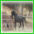
\includegraphics[width=\textwidth]{img/results_discussion/adversarial/adv_unperturbed_framed.png}
        \caption{Original}
    \end{subfigure}
    \hfill
    \begin{subfigure}[b]{0.25\textwidth}
        \centering
        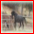
\includegraphics[width=\textwidth]{img/results_discussion/adversarial/adv_pgd_framed.png}
        \caption{PGD, $\ell_\infty$ = 36/255}
    \end{subfigure}
    \hfill
    \begin{subfigure}[b]{0.25\textwidth}
        \centering
        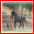
\includegraphics[width=\textwidth]{img/results_discussion/adversarial/adv_fmn_framed.png}
        \caption{FMN}
    \end{subfigure}
    \caption{Original and adversarially-perturbed CIFAR10 observation of class \texttt{horse}. Both perturbations succeed
    at misleading an undefended, pre-trained WideResNet-28-10 architecture.}
\end{figure}

The first results presented correspond to PGD attacks with different attack power 
$\ell_\infty$, namely 8/255, 16/255 and 32/255, for increasing ratio of 
perturbed observations in the CIFAR10 dataset.

\begin{figure}[H]
    \centering
    \begin{subfigure}[b]{\textwidth}
        \centering
        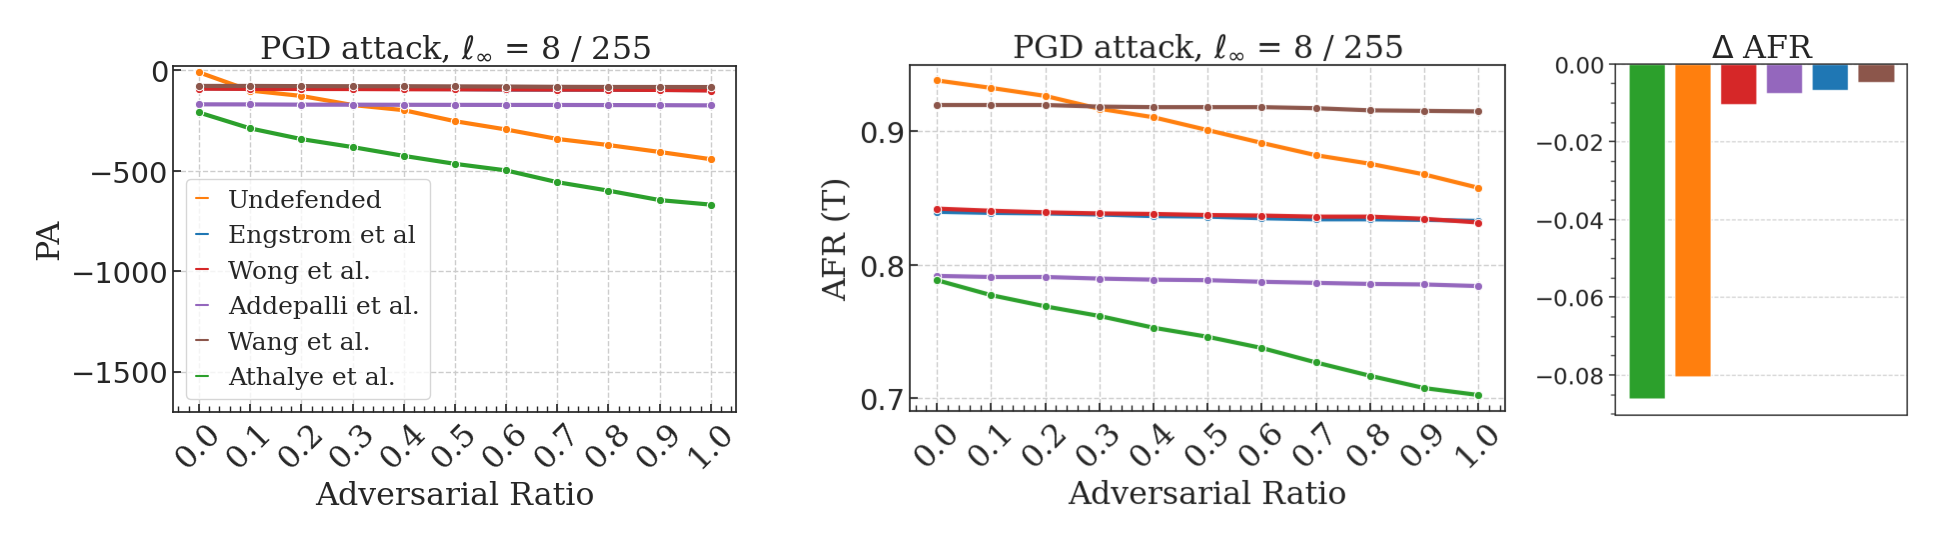
\includegraphics[width=\textwidth]{img/results_discussion/adversarial/PGD_0.0314_combo.png}
    \end{subfigure}

    \vspace{1em}

    \begin{subfigure}[b]{\textwidth}
        \centering
        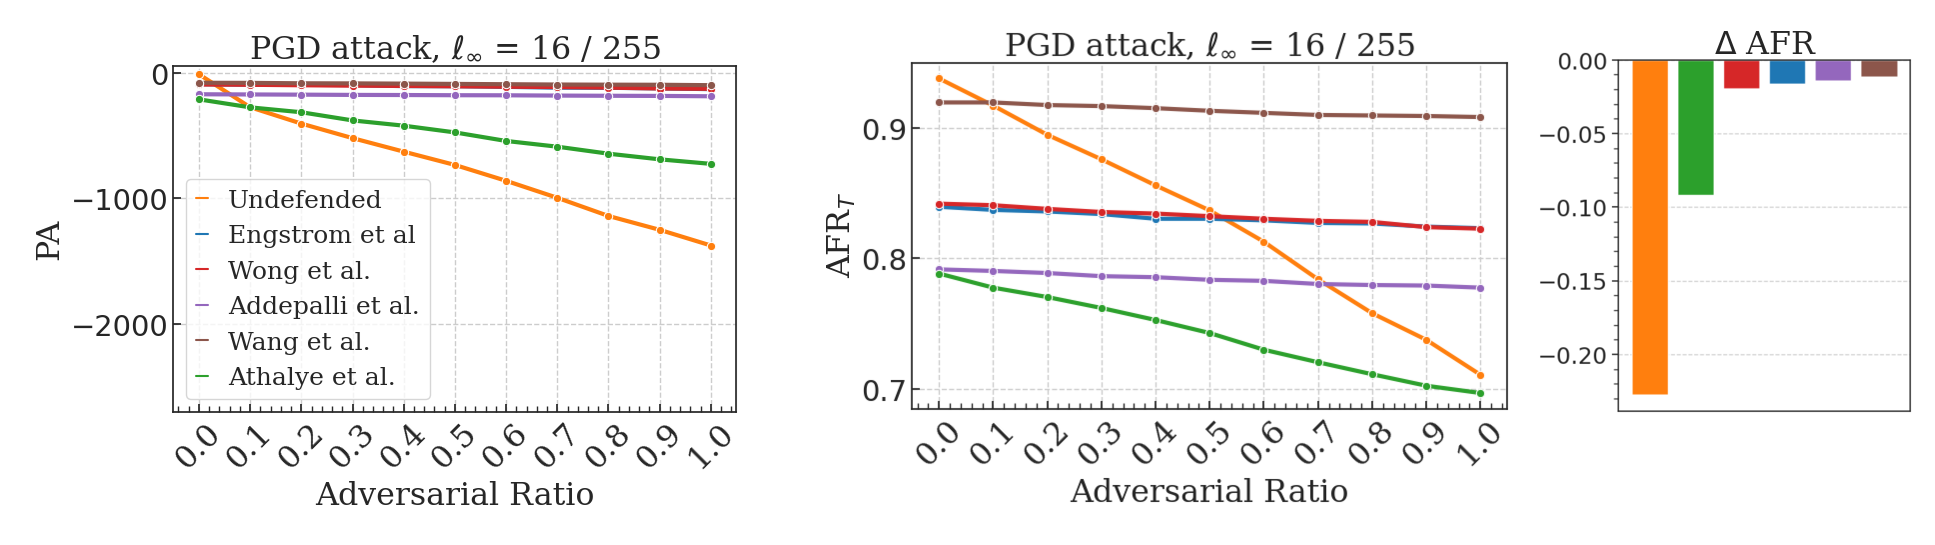
\includegraphics[width=\textwidth]{img/results_discussion/adversarial/PGD_0.0627_combo.png}
    \end{subfigure}

    \vspace{1em}

    \begin{subfigure}[b]{\textwidth}
        \centering
        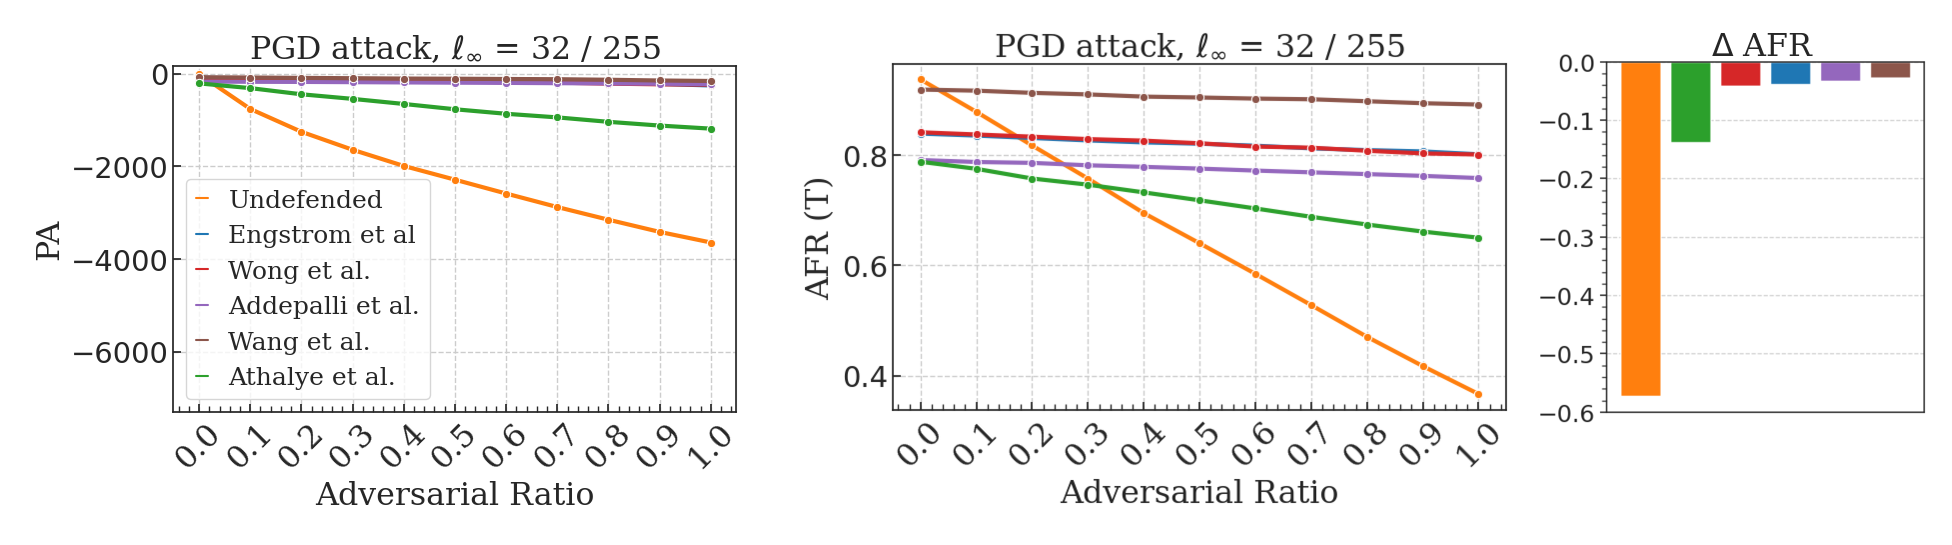
\includegraphics[width=\textwidth]{img/results_discussion/adversarial/PGD_0.1255_combo.png}
    \end{subfigure}

    \caption{PA, $\operatorname{AFR}_\text{T}$ and the AFR variation against increasing adversarial ratio $\alpha \in [0,1]$ at different
    perturbation norm bounds $\ell_\infty$. A pre-trained, undefended WideResNet-28-10
    and five RobustBench \cite{croceRobustBenchStandardizedAdversarial2021a}
    defended models are subject to a 1000 step PGD attack.
    When $\alpha$ = 0, $\operatorname{PA} \longrightarrow 0$ as $\beta \longrightarrow \infty$ in all cases, but
    the convergence rate depends on the prediction confidence (see Figure \ref{fig:prediction_confidence}) and thus yields an assessment equivalent to that
    of $\operatorname{AFR}_\text{T}$.
    }
    \label{fig:six_figures_pa_adv}
\end{figure}

At first glance, it is clear that PA is able to discriminate robust models from
the {\color{tab:orange} \textbf{Undefended}} one, which is shown to significantly
decrease its performance with increasing adversarial ratio and attack power. As expected, 
the rate at which its performance decreases is higher the more powerful the attack is, 
since a greater percentage of observations are misleading. Furthermore, 
it is also clear the {\color{tab:green} \textbf{Athalye et al.}}
is significantly less robust to PGD attacks than its RobustBench counterparts, as 
its performance decreases way more significantly with increasing adversarial ratio. \\

A fundamental difference between these two models, which cannot be
inferred from a purely performance-based metric, is the nature of the misalignment in
the probabilistic output of the model, which is the source of the robust and non-robust
behavior observed. Figure \ref{fig:unrobust_posterior_short_pgd} \textbf{(right)}
shows the optimal $\beta^{*}$ value for each model, which follows
the entropy of the posterior distribution and discriminates the two non-robust
models from the rest and from each other.

\begin{figure}[H]
    \centering
    \begin{subfigure}[b]{\textwidth}
        \centering
        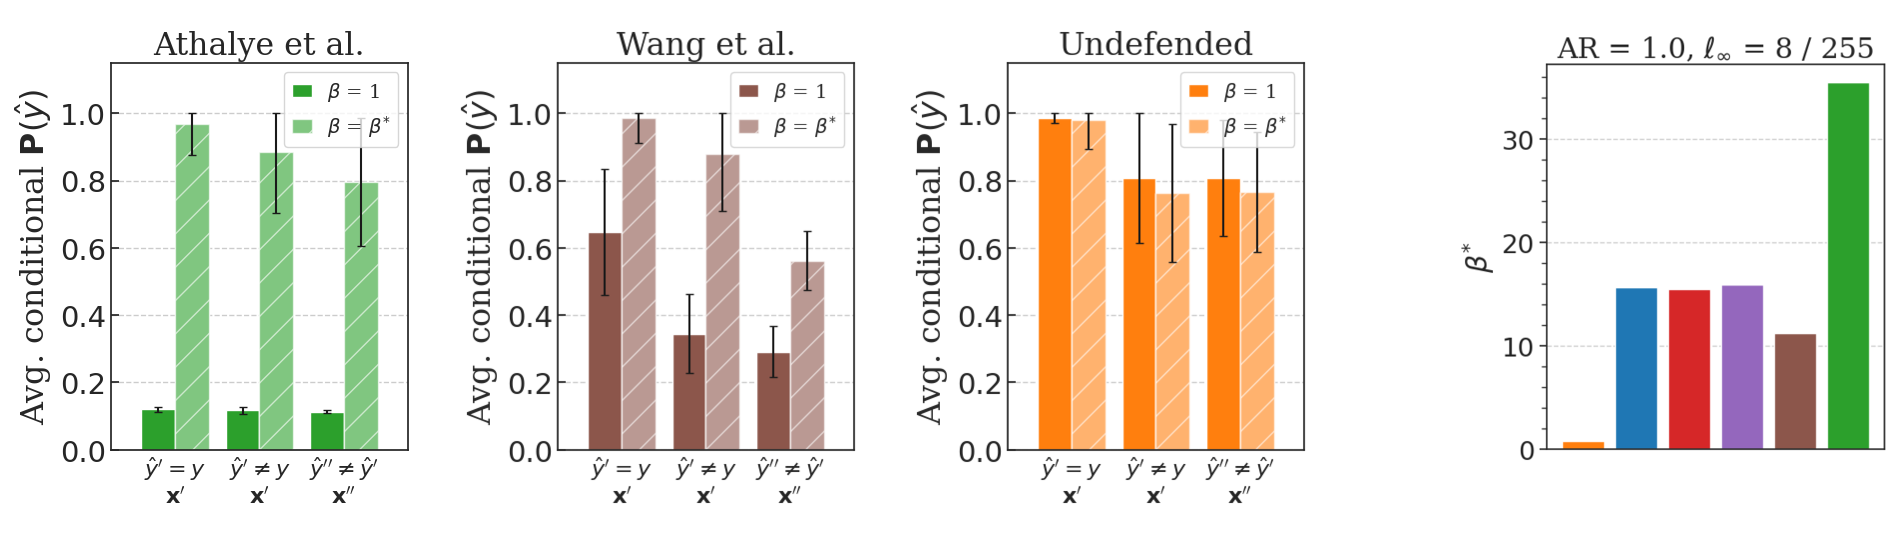
\includegraphics[width=\textwidth]{img/results_discussion/adversarial/bpda_wang_undefended_beta_pgd.png}
    \end{subfigure}
   
    \caption{(\textbf{left}) Average posterior probability of the predicted class for 
    correctly classified original observations, misclassified original observations and 
    misleading adversarial observations. The probabilities assigned to correct 
    ($\hat{y}' = y$) and incorrect ($\hat{y}' \neq y$, $\hat{y}'' \neq y$)
    predictions overlap in both {\color{tab:orange} \textbf{Undefended}} 
    and {\color{tab:green} \textbf{Athalye et al.}} models, whereas the opposite happens for the
    {\color{tab:brown} \textbf{Wang et al.}} case. This highlights
    the suitability of its inductive bias with respect to both sampling randomness and
    adversarial perturbations. (\textbf{right}) Optimal $\beta^{*}$ value achieved by each 
    model. {\color{tab:orange} \textbf{Undefended}} and {\color{tab:green} \textbf{Athalye et al.}} 
    models appear as outliers as they overestimate and underestimate, respectively, the 
    information content of the features. Their poor robustness performance against PGD attacks
    reported in Figure \ref{fig:six_figures_pa_adv} can be explained in these terms.
    These results have been obtained through a PGD attack with $\ell_\infty$=8/255,
    and they are consistent across different values of $\ell_\infty$.
    }
    \label{fig:unrobust_posterior_short_pgd}
\end{figure}

We observe that the {\color{tab:orange} \textbf{Undefended}} model provides overconfident 
predictions that maximize disagreement in misleading and 
misclassified observations, whereas {\color{tab:green} \textbf{Athalye et al.}} provides 
uncertain predictions that minimize disagreement in adversarial observations but have 
the opposite effect in correctly classified ones. The interpretation outlined in
Chapter \ref{sec:theory} contributes to the understanding of these results, as it is shown
that $\beta^{*}$ effectively measures the quality of the informativeness estimation 
made by each model. On the one hand, the {\color{tab:orange} \textbf{Undefended}} 
model overestimates the information content of the features it has learned, and thus overfits 
to these and is unable to generalize under adversarial perturbations. On the other hand, 
{\color{tab:green} \textbf{Athalye et al.}} underestimates the information content and thus
provides overly uncertain predictions. \\

Figure \ref{fig:unrobust_posterior_short_pgd} \textbf{(left)} illustrates
the previous reasoning by displaying the average posterior
probability of the predicted class by each model (i.e. the maximum of the posterior), 
conditioned on the type of prediction assigned. This discrimination yields three groups of observations,
namely original observations that are correctly classified by the model, 
original observations that are misclassified and perturbed examples that, having their 
associated unperturbed observation been correctly classified, 
have been able to mislead the model. These three cases are relevant from the 
adversarial robustness perspective,  as they illustrate the trade-off between high-confident 
original predictions and adversarial vulnerability, which has been already stated in 
previous chapters. {\color{tab:brown} \textbf{Wang et al.}}
acts as a reference for an ideal robust behavior, in which original observations are
predicted with high confidence and adversarially misleading predicted labels are 
only slightly more likely than the rest. Equivalent representations for the remaining
models can be found in Figure \ref{fig:appendix_adversarial_distribution_pgd}. \\

In the case of robust models, we observe a significant difference in the 
discriminative power of PA and accuracy-based metrics that does not immediately
derive from the informativeness of the optimal posterior. As remarked before, AFR$_\text{P}$
constitutes our baseline robustness metric, as by definition represents the ratio
of predictions that remained constant under adversarial perturbations, and
therefore ranks models by their predictive capabilities against these attacks. The
value of $\Delta$AFR aligns with that definition, and discriminates robust models
by a very thin margin, selecting {\color{tab:brown} \textbf{Wang et al.}} as
the best. Further analysis on PA is needed to understand the source of this 
discrepancy, as for instance why {\color{tab:purple} \textbf{Addepalli et al.}} model
is attributed a significantly lower value than the remaining robust models
under a $\ell_\infty$ = 8/255 PGD attack, despite displaying a similar decrease in performance. \\

\begin{table}[H]
    \centering
    \begin{tabular}{l|rrr|rrr}
    Defense & $N_{\text{MIS}}$ & $2 \delta_{\text{MIS}}$ & $\zeta_{\text{SAM}}$ & $N_{\text{ADV}}$ & $\delta_{\text{ADV}}$ & $\zeta_{\text{ADV}}$ \\
    \midrule
    {\color{tab:brown} \textbf{Wang et al.}} & 799 & 0.24 & -468.62 & 47 & 0.44 & -39.44 \\
    {\color{tab:blue} \textbf{Engstrom et al.}} & 1591 & 0.17 & -566.72 & 67 & 0.39 & -63.43 \\
    {\color{tab:red} \textbf{Wong et al.}} & 1562 & 0.17 & -537.25 & 90 & 0.38 & -88.98 \\
    {\color{tab:purple} \textbf{Addepalli et al.}} & 2063 & 0.21 & -877.42 & 75 & 0.46 & -58.92 \\
    {\color{tab:orange} \textbf{Undefended}} & 566 & 0.47 & -736.63 & 810 & 0.24 & -1173.55 \\
    {\color{tab:green} \textbf{Athalye et al.}} & 1915 & 0.23 & -963.85 & 747 & 0.21 & -1183.96 \\
    \bottomrule
    \end{tabular}
    \caption{
    Approximated PA contributions for a PGD attack with $\ell_\infty$ = 8/255 and
    $\alpha = 1.0$. The number of originally misclassified and adversarially misleading
    observations is $N_{\text{MIS}} = \lfloor N (1-\operatorname{AFR}_\text{T}^0) \operatorname{AFR}_\text{P} \rfloor$ and
    $N_{\text{ADV}} = \lfloor N \operatorname{AFR}_\text{T}^0 (1-\operatorname{AFR}_\text{P}) \rfloor$, respectively. 
    The penalization argument $2 \delta_{\text{ERR}}$ has not
    been included for being negligible in all cases.
    }
    \label{tab:approx_pa_pgd_table}
\end{table}

Table \ref{tab:approx_pa_pgd_table} shows the contribution of each subset of observations to the final
approximated PA value for a PGD attack. $N_{\text{ERR}}$, $N_{\text{MIS}}$ and $N_{\text{ADV}}$ are 
the number of pairs of contributing observations, and $\zeta_{\text{ERR}}$, $\zeta_{\text{MIS}}$ and $\zeta_{\text{ADV}}$ are
the total amount of the contribution. For reasons described earlier in this section,
the PA approximation overestimates penalizations when compared to the true value, but
relative discrepancies between models are still largely preserved and therefore the rationale
behind the discriminative power of PA, as shown in Figures \ref{fig:appendix_adversarial_approx_pa_pgd}
and \ref{fig:appendix_adversarial_approx_pa_fmn}. The parameters $2 \delta_{\text{MIS}}$ and
$\delta_{\text{ADV}}$ account for the average probability assigned to classes other than the predicted
class for misclassified original observations and misleading adversarial observations, respectively, and 
help interpret the informativeness of the distribution as well as the value of each individual 
penalization. \\

For instance, a large $2 \delta_{\text{MIS}}$ value indicates robustness to sampling randomness, as it
represents higher average uncertainty in misclassified predictions. A model with a high performance on 
test data entails a more negative penalization $\log(1 - 2 \delta_{\text{MIS}})$, for being misclassified 
observations more likely to be equivalently misclassified under adversarial perturbations, but at
the same time makes misclassifications less likely, and therefore the number of terms added to
$\zeta_{\text{MIS}}$. The existing trade-off between standard and robust generalization arises when 
following this reasoning towards the minimization of $\zeta_{\text{MIS}}$, because reducing the number of 
misclassified observations will drive $\beta^{*}$ to higher values and therefore decrease adversarial 
uncertainty $\delta_{\text{ADV}}$. As outlined before, $\delta_{\text{ADV}}$ indicates 
robustness to adversarial perturbations, as it represents the average prediction uncertainty on adversarial 
misleading observations, and entails a penalization of $\log(\delta_{\text{ADV}})$. \\

The interpretation of these terms is vitally important for the purpose of this work, as it enables
the identification of the different sources of robustness displayed by each model, and therefore
the characterization of the randomness that we will demand models to generalize to. From a general 
perspective, $\zeta_{\text{SAM}} = \zeta_{\text{ERR}} + \zeta_{\text{MIS}}$ can be understood as the lack of robustness
to sampling randomness, and $\zeta_{\text{ADV}}$ as the lack of robustness to adversarial perturbations. \\

As expected, the standard generalization error term $\zeta_{\text{SAM}}$ is the one contributing most to
the PA measure in robust models, as the selected PGD attack is not very effective and can only generate
a few misleading observations $N_{\text{ADV}}$. The discrimination of models based exclusively 
on $\zeta_{\text{SAM}}$  is very much aligned with that of $\operatorname{AFR}_\text{T}$ in all cases except for the
{\color{tab:orange} \textbf{Undefended}} model, which is penalized more heavily for providing
overconfident predictions with numerous misleading examples $N_{\text{ADV}}$ and
thus converging to a small $\beta^{*}$. This is an important realization, as it shows that even if
standard and adversarial robustness contributions can be dissociated, they are mutually dependent
and ultimately derive from the overall agreement in all predictions, regardless of the nature of the
randomness they are bound to. The generalization error to sampling randomness will be exceedingly penalized
the less robust a model is to other sources of randomness, because the optimal resolution of the hypothesis
space is reduced and the less distinction can be made between adversarial observations and outliers from
the original dataset. \\

Further insights can be obtained by comparing these results
with those of the {\color{tab:green} \textbf{Athalye et al.}} model, which has a similar accuracy
on adversarial observations and a significantly worse accuracy on original observations. The fact that posterior
distributions are profoundly uninformative increases agreement in between mismatching posterior and
thus lowers penalization terms, even if more terms will be added as a consequence of the
associated decrease in performance. \\

The same reasoning can be followed to explain the discrimination made by PA between
{\color{tab:purple} \textbf{Addepalli et al.}} and the other robust models. {\color{tab:purple} \textbf{Addepalli et al.}}
experiences a comparable drop in performance, and for displaying a reduced confidence in mismatching predictions
is assigned a smaller $\zeta_{\text{SAM}}$ contribution than some of these models. Nevertheless, such 
uncertainty is also observed for original observations, which lowers accuracy on the original dataset 
and thus increases random sampling penalization $\zeta_{\text{SAM}}$. In that sense, it can be argued
that {\color{tab:purple} \textbf{Addepalli et al.}} is more robust than {\color{tab:red} \textbf{Wong et al.}}
and {\color{tab:blue} \textbf{Engstrom et al.}} to adversarial perturbations, which also stems from
the baseline AFR$_\text{P}$ and $\Delta$AFR values, but significantly less robust to sampling randomness.
PA weights both contributions and yields an intermediate model selection criterion. \\

Regarding adversarial robustness, we observe that $\zeta_{\text{ADV}}$ is driven by the decrase in 
performance under attack $\Delta$AFR, as $N_{\text{ADV}}$ penalization terms
are added. Nevertheless, the value of each of these terms is $\log(\delta_{\text{ADV}})$, which penalizes
models that achieve maximum posterior agreement by increasing confidence on adversarially
misleading examples. This is a clear distinctive trait with respect to accuracy-based metrics,
whose penalizations are reduced to a binary decision. \\

Figure \ref{fig:pgd_eps} shows that PA is also discriminative with respect to
increasing attack power, expressed through the maximum allowed $\ell_\infty$ norm. 
As mentioned earlier, PA values are heavily aligned with the performance
decrease of the models under a specific attack power, but the observed decrease in PA 
under increasing $\ell_\infty$ is much more significant than the decrease 
in performance. This can be explained by the fact that the metric is sensitive 
to the overall posterior shift and not only the position of the maximum. When increasing 
the attack power, confidence in the predicted class will decrease in general, 
even when the observation does not succeed at misleading the model, and therefore the
overall overlap between posteriors will be reduced even at comparable performance 
levels. This observation further illustrates the independent discriminability power
offered by PA (see Properties \ref{properties:robustness}), which constitutes the 
cornerstone argument of this work. \\

\begin{figure}[b]
    \centering
    \begin{subfigure}[b]{0.37\textwidth}
        \centering
        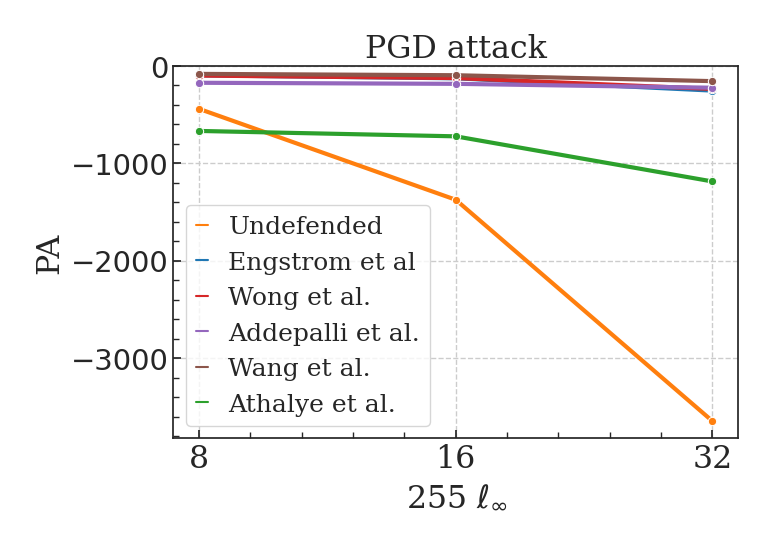
\includegraphics[width=\textwidth]{img/results_discussion/adversarial/PGD_logPA_eps.png}
    \end{subfigure}
    \hfill
    \begin{subfigure}[b]{0.59\textwidth}
        \centering
        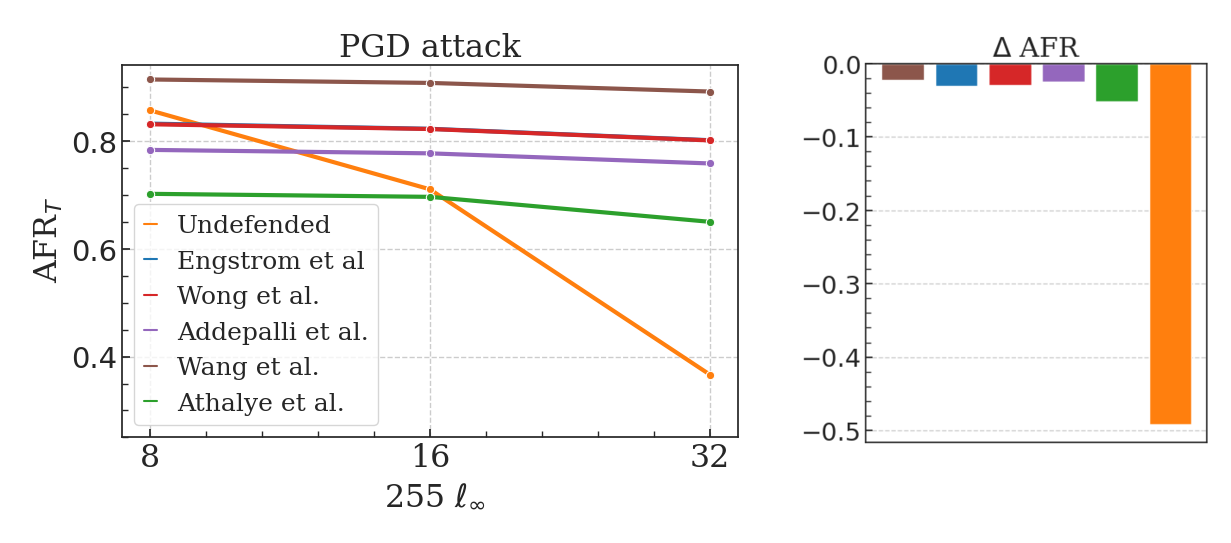
\includegraphics[width=\textwidth]{img/results_discussion/adversarial/PGD_AFR_true_eps_diff.png}
    \end{subfigure}
    \caption{PA, $\operatorname{AFR}_\text{T}$ and the AFR variation against increasing attack power for  $\alpha = 1$. 
    The undefended net and several RobustBench robust models are considered
    under a 1000 step PGD attack.}
    \label{fig:pgd_eps}
\end{figure}

In order to widen the scope of the analysis, analogous results are obtained for
FMN attacks, which are expected to be more effective than PGD attacks for being 
unbounded and lead to smaller $\beta^{*}$ values (see 
Table \ref{tab:entropy_gibbs}). Figure \ref{fig:adv_fmn_pa_afr} shows the evolution 
of PA against increasing adversarial ratio for the same models, and compares
it with the assessment provided by AFR.


\begin{figure}[H]
    \centering
    \begin{subfigure}[b]{0.39\textwidth}
        \centering
        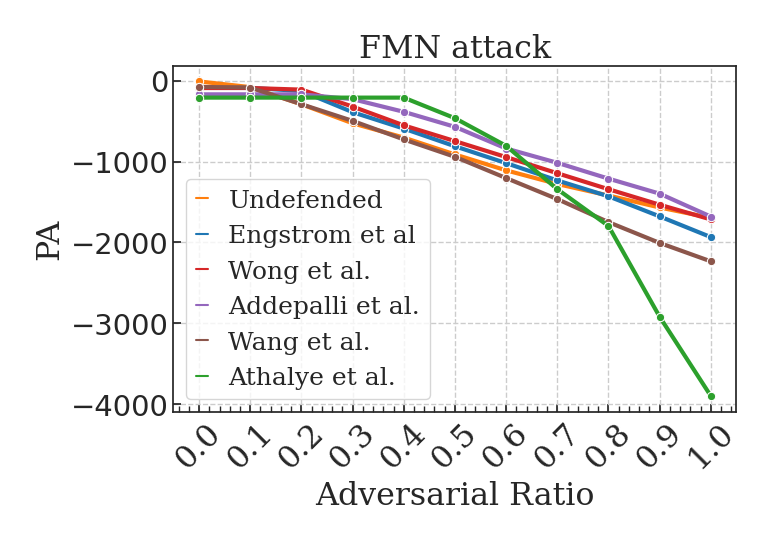
\includegraphics[width=\textwidth]{img/results_discussion/adversarial/FMN_logPA.png}
    \end{subfigure}
    \hfill
    \begin{subfigure}[b]{0.59\textwidth}
        \centering
        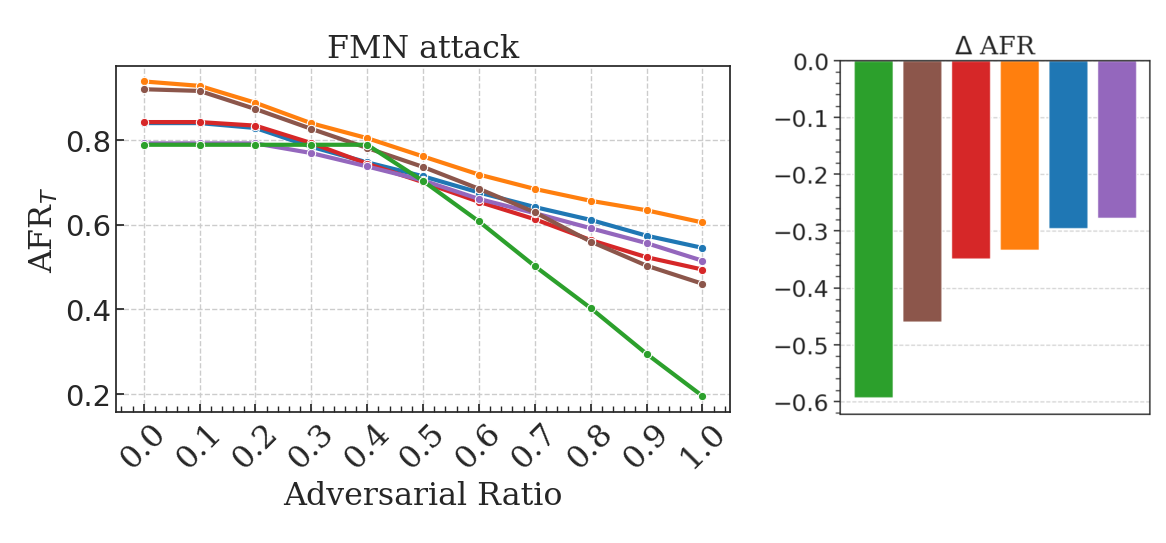
\includegraphics[width=\textwidth]{img/results_discussion/adversarial/FMN_1000_AFR_true.png}
    \end{subfigure}
    \caption{PA, $\operatorname{AFR}_\text{T}$ and the AFR variation against increasing adversarial ratio. 
    The undefended net and several RobustBench robust models are considered 
    under a 1000 step FMN attack.}
    \label{fig:adv_fmn_pa_afr}
\end{figure}


As expected, the effectiveness of the FMN attack is superior to that of PGD attacks, as
the decrease in performance is substantially more significant for all models, especially the ones
previously considered robust. It must be noted that the adversarial ratio must be interpreted differently
in this case, because the perturbations introduced are sorted by norm. 
In  particular, an adversarial ratio $\alpha$ comprises perturbations up to the $\alpha$ quantile
of the norm distribution. The consistency in the assessment provided by PA is lost for this 
reason, as prediction confidence is not constant across $\alpha$ values but instead decreases
monotonically with it, which will trigger a different robustness response in each model. \\

It stems from these results that robust models have been defended with a
compression strategy that succeeds at filtering out small perturbations, and for that 
reason maintain their performance at low adversarial ratio values \cite{dasKeepingBadGuys2017}.
In particular, {\color{tab:green} \textbf{Athalye et al.}} remains maximally robust
until at least 40\% of the observations are perturbed, at which point the defensive strategy
is neutralized and a constant fraction of the additional perturbed observations succeeds at
misleading the model, which translates into a linear decrease in performance and PA. \\

PA proves to be very discriminative among robust models and to represent the 
phase transition entailed by the collapse of the defense strategy better than AFR does, which can be
observed in more detail in Figure \ref{fig:appendix_adversarial_afrpred_fmn}. A significative
result is that PA is not so directly aligned with $\Delta$AFR, in contrast to
the PGD case, which shows again that the decrease in performance is not the main driver of
the robustness assessment provided by PA, but instead can be interpreted as a consequence of
a misalignment in the posterior distributions of adversarial observations, which are the ones driving
the metric after the $\alpha$ threshold is reached. \\

\begin{figure}[H]
    \centering
    \begin{subfigure}[b]{\textwidth}
        \centering
        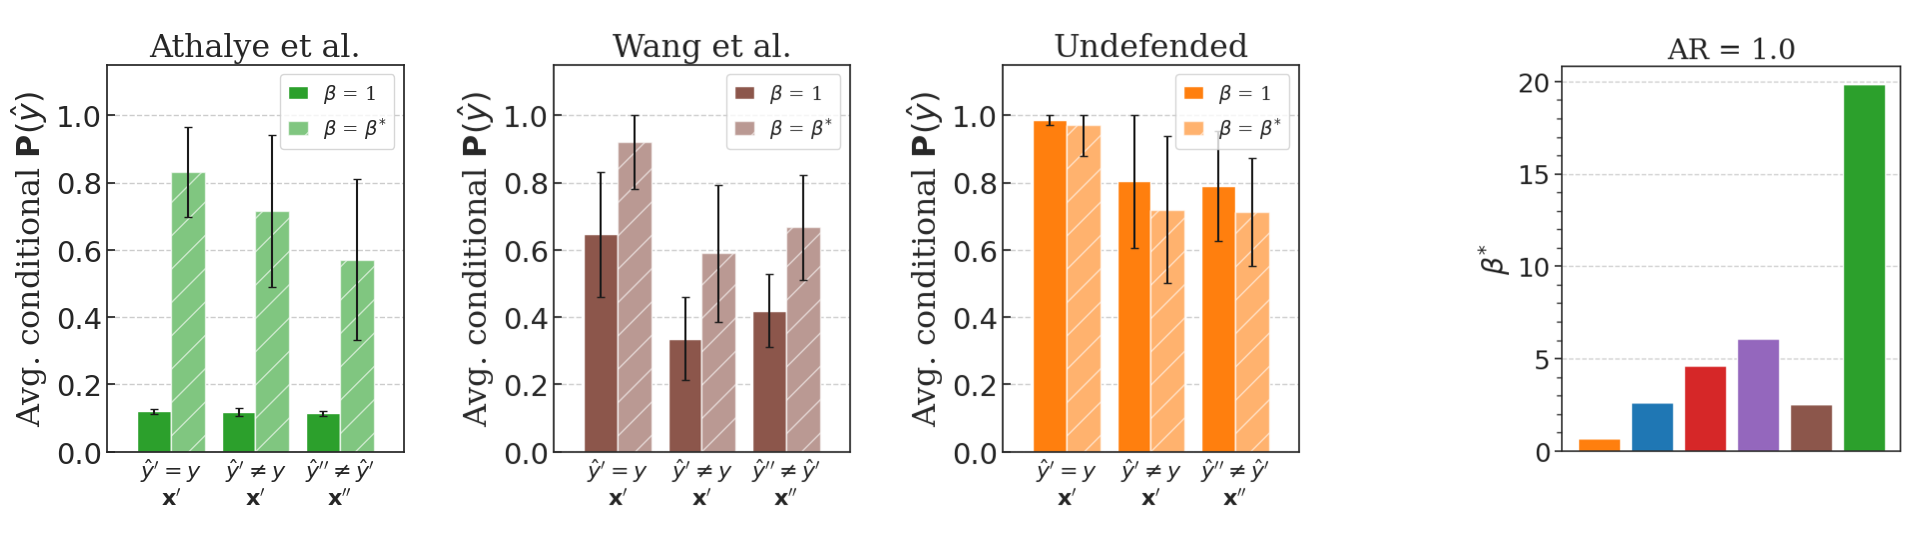
\includegraphics[width=\textwidth]{img/results_discussion/adversarial/bpda_wang_undefended_beta_fmn.png}
    \end{subfigure}
   
    \caption{(\textbf{left}) Average posterior probability of the predicted class under
    FMN attack for correctly classified original observations, misclassified original observations, and 
    misleading adversarial observations. The probabilities assigned to correct 
    ($\hat{y}' = y$) and incorrect ($\hat{y}' \neq y$, $\hat{y}'' \neq y$)
    predictions are shown to overlap also for the {\color{tab:brown} \textbf{Wang et al.}}
    model, which highlights the effectiveness of the FMN attack with respect to PGD.
    (\textbf{right}) Optimal $\beta^{*}$ value for each model.
    % These results have been obtained through a FMN attack.
    }
    \label{fig:unrobust_posterior_short_fmn}
\end{figure}

Figure \ref{fig:unrobust_posterior_short_fmn} gives insight into the probabilistic output
of the model and the informativeness of the optimal posterior for the {\color{tab:orange} \textbf{Undefended}}, 
{\color{tab:green} \textbf{Athalye et al.}} and {\color{tab:brown} \textbf{Wang et al.}} models, in
analogous way to the PGD experiments. The first two models display a very similar behavior for 
$\beta = 1$, but optimal posteriors are less informative due to the increased number of misleading
observations, which translates into a smaller $\beta^{*}$. The response of 
the {\color{tab:brown} \textbf{Wang et al.}} model further illustrates the higher effectiveness of
FMN attacks, as adversarial perturbations are on average more misleading than outlier observations in
the original dataset, which did not occur in the PGD case. Analogous representations for the remaining
models can be found in Figure \ref{fig:appendix_adversarial_distribution_fmn}, which show
that the {\color{tab:purple} \textbf{Addepalli et al.}} is the only robust model that maintains
the same behavior under both attacks.\\

Finally, Table \ref{tab:approx_pa_fmn_table} displays the approximated PA contributions for the FMN attack.
In contrast with the PGD case, FMN is much more effective and $N_{\text{ADV}} > N_{\text{MIS}}$
in all cases, which makes the adversarial contribution $\zeta_{\text{ADV}}$ more relevant in the
overall robustness assessment. The discrepancy observed between PA and
accuracy-based metrics for the {\color{tab:red} \textbf{Wong et al.}} model can also be explained 
in these terms, as it is the least penalized by $\zeta_{\text{SAM}}$ among robust models due to its
superior accuracy. In the context of effective attacks, predictive certainty on
original observations is highly rewarded because lower overall agreement makes sampling penalization terms
$\log(1 - 2 \delta_{\text{MIS}})$ more negative. \\

\begin{table}[b]
    \centering
    \begin{tabular}{l|rrr|rrr}
    Defense & $N_{\text{MIS}}$ & $2 \delta_{\text{MIS}}$ & $\zeta_{\text{SAM}}$ & $N_{\text{ADV}}$ & $\delta_{\text{ADV}}$ & $\zeta_{\text{ADV}}$ \\
    \midrule
    {\color{tab:purple} \textbf{Addepalli et al.}} & 1507 & 0.52 & -1910.69 & 2187 & 0.28 & -2788.89 \\
    {\color{tab:red} \textbf{Wong et al.}} & 1032 & 0.46 & -1125.53 & 2920 & 0.27 & -3844.40 \\
    {\color{tab:blue} \textbf{Engstrom et al.}} & 1125 & 0.72 & -2469.65 & 2505 & 0.32 & -2847.99 \\
    {\color{tab:brown} \textbf{Wang et al.}} & 435 & 0.82 & -1599.08 & 4215 & 0.33 & -4637.45 \\
    {\color{tab:orange} \textbf{Undefended}} & 412 & 0.56 & -704.58 & 3132 & 0.29 & -3906.55 \\
    {\color{tab:green} \textbf{Athalye et al.}} & 859 & 0.57 & -2054.23 & 4679 & 0.43 & -3955.43 \\
    \bottomrule
    \end{tabular}
    \caption{
    Approximated PA contributions for a FMN attack with $\alpha = 1.0$. The number of 
    originally misclassified and adversarially misleading
    observations is $N_{\text{MIS}} = \lfloor N (1-\operatorname{AFR}_\text{T}^0) \operatorname{AFR}_\text{P} \rfloor$ and
    $N_{\text{ADV}} = \lfloor N \operatorname{AFR}_\text{T}^0 (1-\operatorname{AFR}_\text{P}) \rfloor$, respectively. 
    The penalization argument $2 \delta_{\text{ERR}}$ has not
    been included for being negligible in all cases except for the 
    {\color{tab:green} \textbf{Athalye et al.}} model, which amounts to 0.36. 
    }
    \label{tab:approx_pa_fmn_table}
    \end{table}

Overall, we recognize that PA has a higher discriminative power than AFR, especially
considering the evolution of each metric over increasing adversarial ratio, as
seen in Figures \ref{fig:six_figures_pa_adv} and \ref{fig:adv_fmn_pa_afr}. 
In particular, Figures \ref{fig:appendix_adversarial_afrpred_pgd} and \ref{fig:appendix_adversarial_afrpred_fmn}
compare the evolution of PA with that of AFR$_\text{P}$, which is the baseline metric for robustness,
and show the susceptibility of the latter to dataset variability. This is an important
consideration, as PA not only improves the discriminability in terms of the scale of
the differences between models, but also provides a more stable assessment across varying
proportion of perturbed observations, under which AFR$_\text{P}$ exhibits significant fluctuations
that alter the ranking of the models at every step, as illustrated in 
Tables \ref{tab:pa_afrpred_comparison_table}. \\

\begin{table}[h]
    \centering
    \resizebox{\textwidth}{!}{%
    \begin{tabular}{l|ccc|ccc|ccc}
    \multirow{2}{*}{} & \multicolumn{3}{c|}{$\alpha$ = 2/10} & \multicolumn{3}{c|}{$\alpha$ = 4/10} & \multicolumn{3}{c}{$\alpha$ = 6/10} \\
    % \cmidrule{2-10}
    \textbf{PGD} & PA & $\operatorname{AFR}_{\text{P}}$ & $\operatorname{AFR}_{\text{T}}$ & PA & $\operatorname{AFR}_{\text{P}}$  & $\operatorname{AFR}_{\text{T}}$ & PA & $\operatorname{AFR}_{\text{P}}$  & $\operatorname{AFR}_{\text{T}}$ \\
    \midrule
    {\color{tab:purple} \textbf{Addepalli et al.}} & \textbf{-172.5} & \textbf{0.995} & \textbf{0.785} & \textbf{-175.5} & 0.992  & \textbf{0.786} & \textbf{-177.6} & 0.989  & \textbf{0.783} \\
    {\color{tab:red} \textbf{Wong et al.}} & -97.7 & 0.996  & 0.838 & -102.9 & 0.992  & 0.834 & -109.2 & \textbf{0.987}  & 0.830 \\
    {\color{tab:blue} \textbf{Engstrom et al.}} & -94.2 & 0.996 & 0.836 & -104.6 & \textbf{0.990} & 0.830 & -110.3 & 0.988 & 0.829 \\
    {\color{tab:brown} \textbf{Wang et al.}} & -81.9 & 0.997 & 0.917 & -84.6 & 0.996 & 0.915 & -89.4 & 0.991 & 0.912 \\
    \midrule
    \addlinespace
    \addlinespace
    \textbf{FMN} & PA & $\operatorname{AFR}_{\text{P}}$ & $\operatorname{AFR}_{\text{T}}$ & PA & $\operatorname{AFR}_{\text{P}}$  & $\operatorname{AFR}_{\text{T}}$ & PA & $\operatorname{AFR}_{\text{P}}$  & $\operatorname{AFR}_{\text{T}}$ \\
    \midrule
    {\color{tab:purple} \textbf{Addepalli et al.}} & -169.4 & 1.0 & \textbf{0.791} & -385.4 & 0.944  & \textbf{0.737} & --838.9 & 0.867  & 0.660 \\
    {\color{tab:red} \textbf{Wong et al.}} & -111.2 & 0.991  & 0.834 & -553.1 & 0.901  & 0.743 & -944.8 & 0.810  & \textbf{0.653} \\
    {\color{tab:blue} \textbf{Engstrom et al.}} & -128.5 & 0.988 & 0.828 & -592.9 & 0.907 & 0.747 & -1020 & 0.836 & 0.675 \\
    {\color{tab:brown} \textbf{Wang et al.}} & \textbf{-291.6} & \textbf{0.952} & 0.873 & \textbf{-726.8} & \textbf{0.861} & 0.781 & \textbf{-1204} & \textbf{0.764} & 0.684 \\
    \bottomrule
    \end{tabular}%
    }
    \caption{
        Comparison of PA, $\operatorname{AFR}_{\text{P}}$ and $\operatorname{AFR}_{\text{T}}$ scores for a 
        PGD attack with $\ell_\infty$ = 16 / 255 and an FMN attack across different adversarial 
        ratio values. Among robust models, the worst robustness score is emboldened for every case.
        PA displays higher consistency and discriminative power across varying $\alpha$ with respect to 
        accuracy-based metrics. In the PGD case, PA is aligned with $\operatorname{AFR}_{\text{T}}$ because
        sampling randomness is the principal source of unrobustness. In the FMN case, PA is aligned with 
        $\operatorname{AFR}_{\text{P}}$ because adversarial perturbations are the principal source of unrobustness.
    }
    \label{tab:pa_afrpred_comparison_table}
\end{table}

Furthermore, the analysis of the approximated robustness contributions highlights the fact that 
the final PA value stems from a combination of standard and adversarial generalization error, which 
are normally obtained independently through different accuracy-based metrics, and leads to 
the realization that PA provides an intermediate assessment in between AFR measures. An analogous 
combined metric weighting accuracy and $\Delta$AFR would not be equiparable to PA, given that these 
weights would be arbitrary and would not adjust to the particularities of each model. For instance, the 
{\color{tab:orange} \textbf{Undefended}} model should be mostly penalized on the basis of its
robustness to adversarial examples, whereas {\color{tab:purple} \textbf{Addepalli et al.}}
model should be mostly penalized for its lack of robustness to sampling randomness in the
original data. These considerations are fundamental in the covariate shift setting, as
different models with different defensive or invariant feature learning strategies will
navigate the generalization-complexity trade-off differently.

As a conclusion to the analysis, several discrepancy measures between 
the model's representation of $\bm{x}'$ and $\bm{x}''$ have been considered, so that it can be 
determined whether they are able to discriminate robust models with a similar power as that of PA. 
On the one hand, posterior-based metrics such as Kullback-Leibler divergence 
and Wasserstein distance have been considered, each providing a notion of discrepancy between
probability distributions. On the other hand, different distance measures in the latent space of
feature representations were considered, including cosine similarity, centroid distance,
and other cluster-based approaches like maximum mean discrepancy and Fr\'echet inception distance 
(FID). FID is particularly relevant, as it is a widely used metric in the generative adversarial network 
literature and thus fits intuitively well into our setting. \\

\begin{figure}[H]
    % \centering
    % 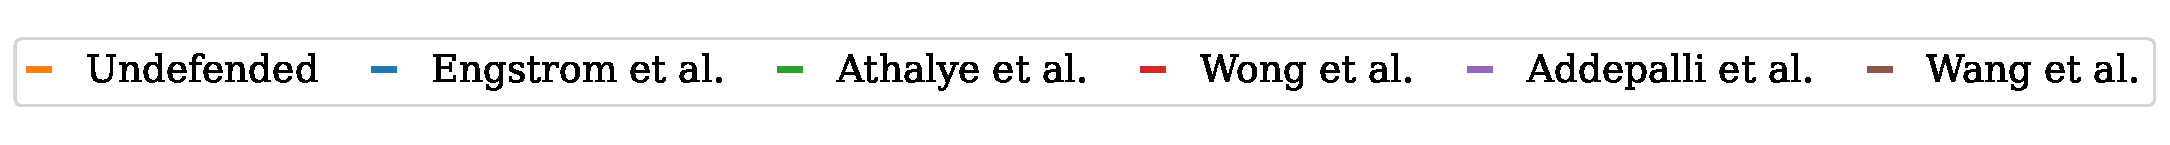
\includegraphics[width=\linewidth,clip]{img/legend_horizontal.pdf}

    \centering
    \begin{subfigure}[b]{0.5\textwidth}
        \centering
        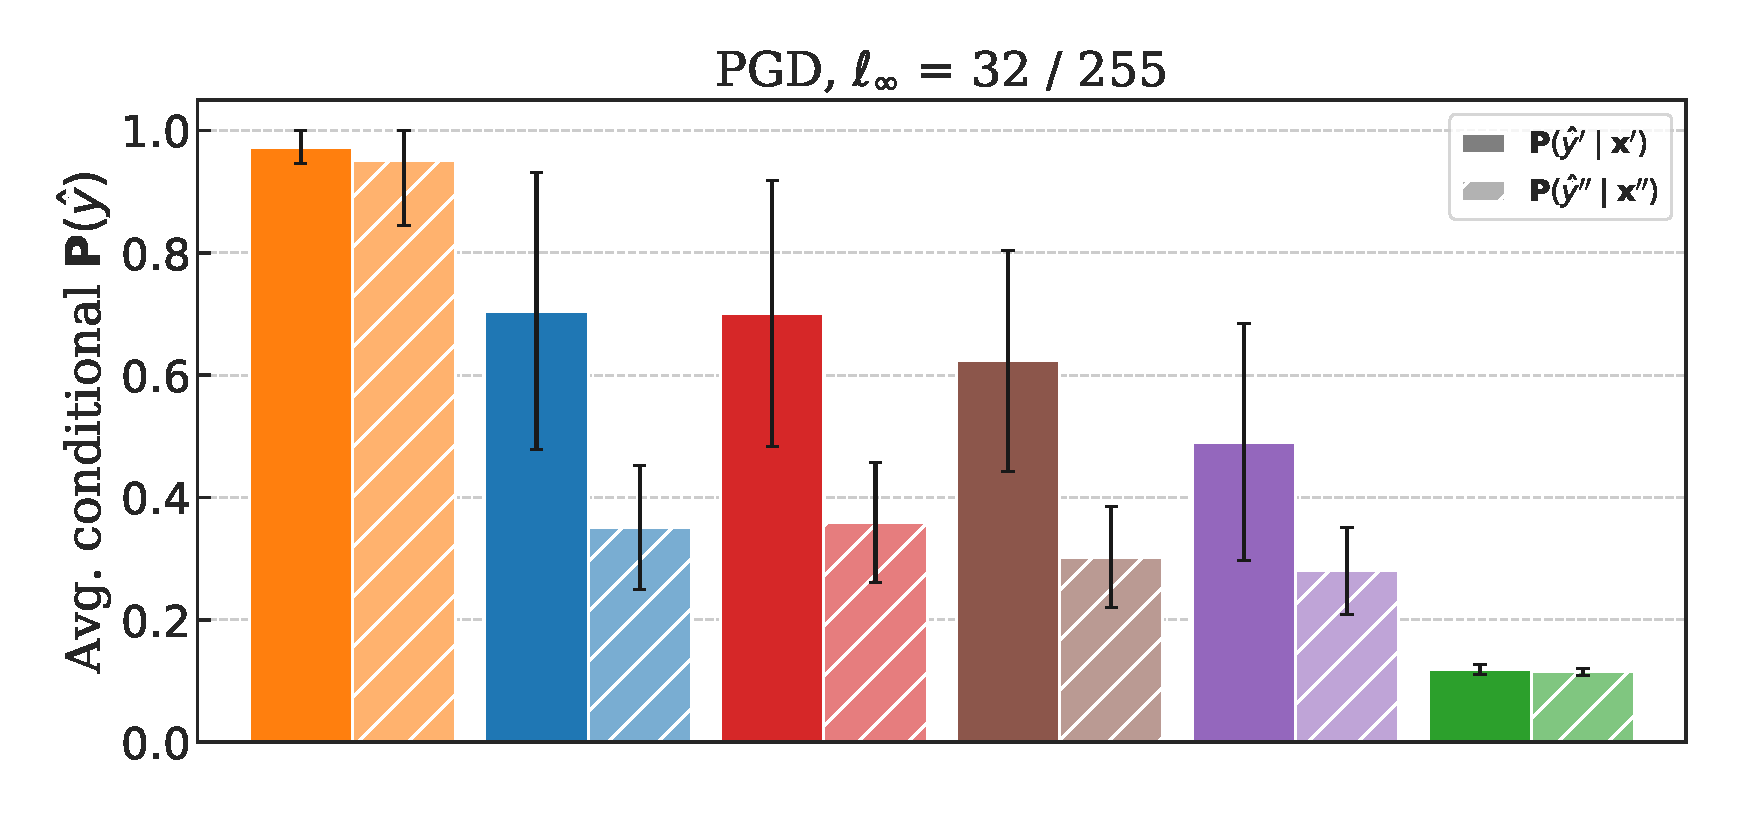
\includegraphics[width=\textwidth]{img/results_discussion/adversarial/2_PGD_0.1255_thesis2.pdf}
    \end{subfigure}
    \hfill
    \begin{subfigure}[b]{0.23\textwidth}
        \centering
        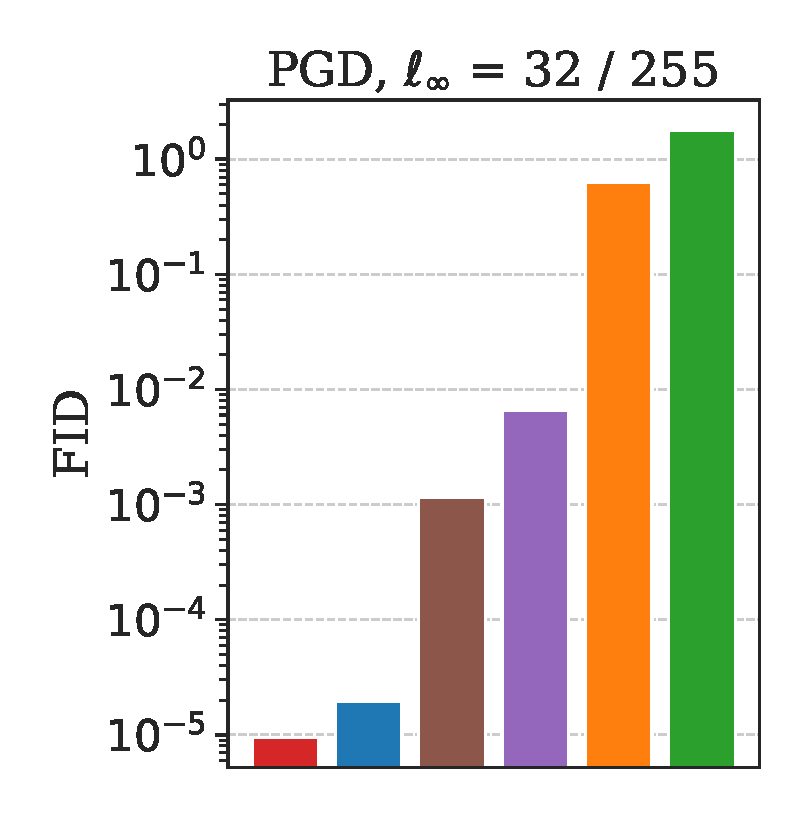
\includegraphics[width=\textwidth]{img/results_discussion/adversarial/FID_barplot_0.1255_300.pdf}
    \end{subfigure}
    \begin{subfigure}[b]{0.23\textwidth}
        \centering
        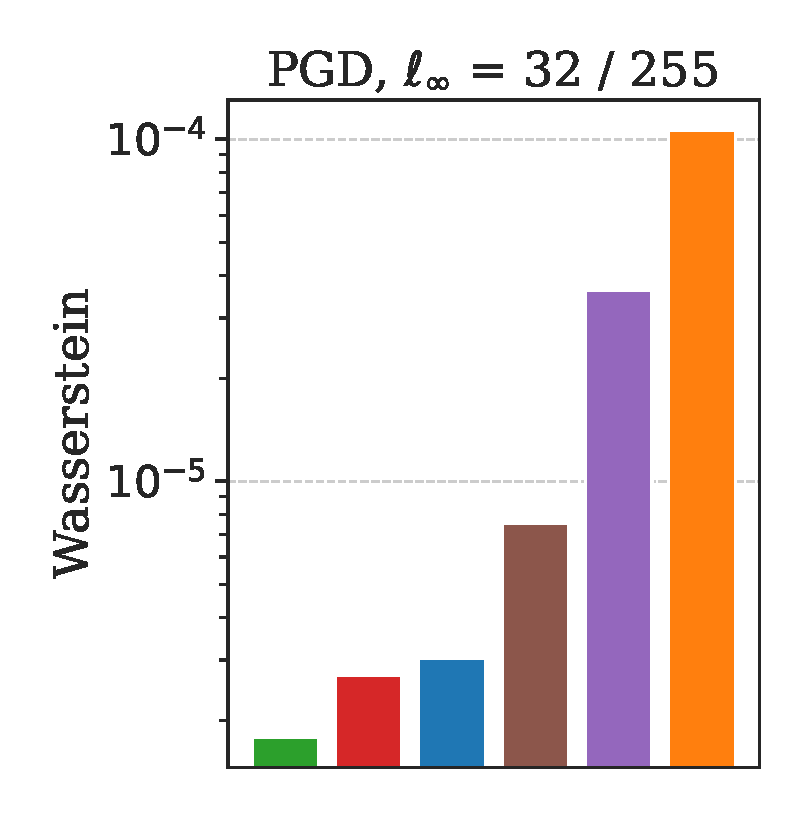
\includegraphics[width=\textwidth]{img/results_discussion/adversarial/W_barplot_0.1255_300.pdf}
    \end{subfigure}

    \vspace{1em}

    \begin{subfigure}[b]{0.5\textwidth}
        \centering
        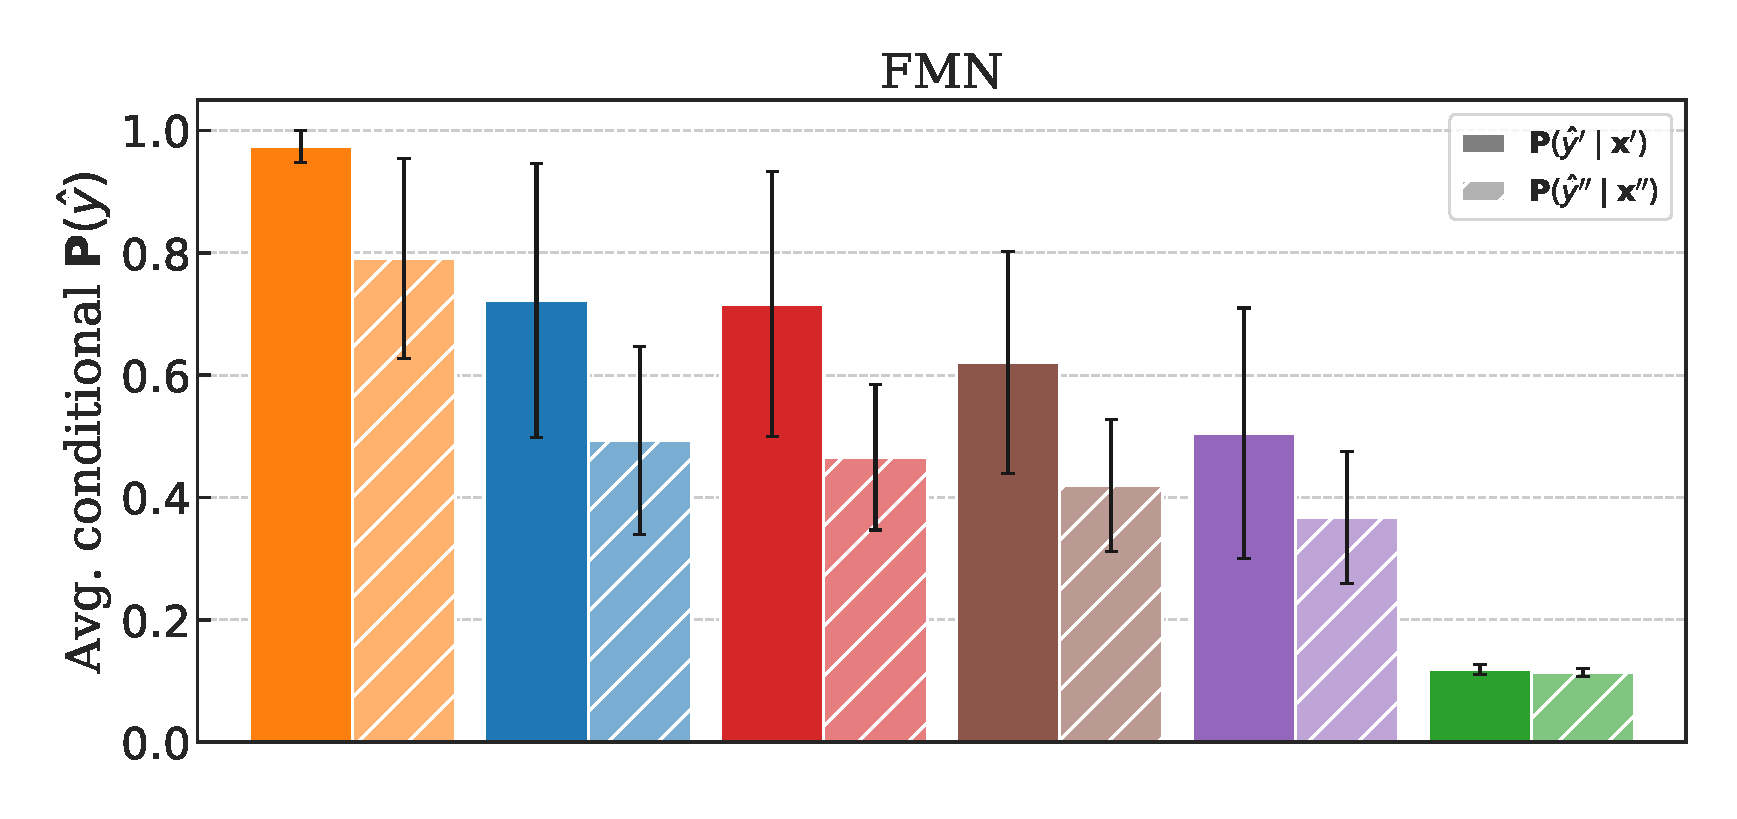
\includegraphics[width=\textwidth]{img/results_discussion/adversarial/2_FMN_thesis2.pdf}
    \end{subfigure}
    \hfill
    \begin{subfigure}[b]{0.23\textwidth}
        \centering
        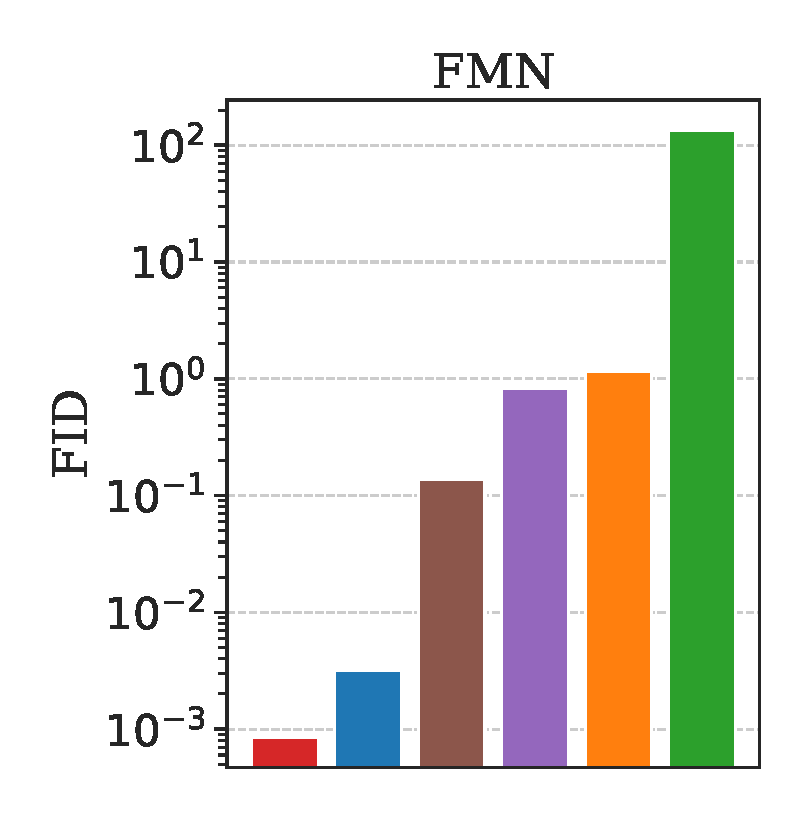
\includegraphics[width=\textwidth]{img/results_discussion/adversarial/FID_barplot_FMN_300.pdf}
    \end{subfigure}
    \begin{subfigure}[b]{0.23\textwidth}
        \centering
        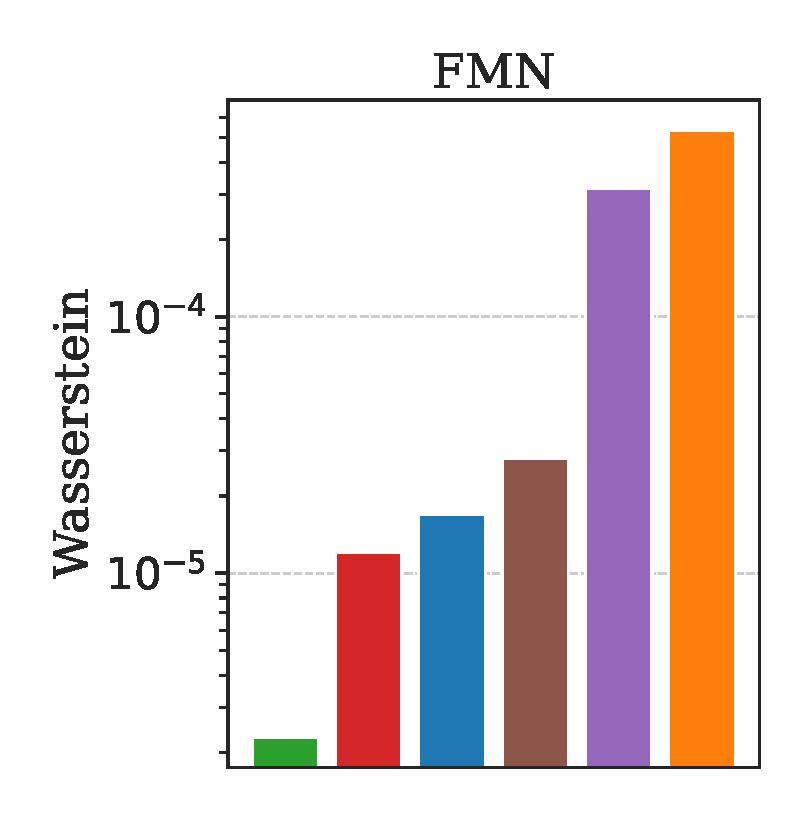
\includegraphics[width=\textwidth]{img/results_discussion/adversarial/W_barplot_FMN_300.pdf}
    \end{subfigure}

    \caption{(\textbf{left}) Average posterior probability of the predicted class in the original and perturbed
    datasets with $\alpha = 1$. (\textbf{middle}) Average Fr\'echet Inception Distance (FID) between feature space 
    representations of $\bm{x}'$ and $\bm{x}''$. (\textbf{right}) Average Wasserstein (W) distance between posteriors
    $\mathbf{P}^f(\cdot | \bm{x'})$ and $\mathbf{P}^f(\cdot | \bm{x''})$ at $\beta_0 = 1$. 
    }
    \label{fig:adv_metric_comparison}
\end{figure}

Figure \ref{fig:adv_metric_comparison} displays the FID and Wasserstein distance values for
all models with $\alpha=1$, for both PGD and FMN attacks, together with a representation
of the average posterior for the original and perturbed datasets
at $\beta_0 = 1$. Both metrics preserve the relative ordering of the models across different attacks, 
and their discriminative power does not appear to correlate with the baseline robustness 
and performance metrics considered. On the one hand, posterior distance is biased
towards low-informative distributions, and for that reason yields the smallest value to 
the {\color{tab:green} \textbf{Athalye et al.}} model. In this model, the overlap between
posteriors is the smallest in absolute terms but the largest in proportion, which constitutes the
main source of generalization error. On the other hand, the FID between feature 
space representations yields a high value for models with significant posterior overlap, 
which serves as a first-order indicator of the quality of the 
inductive bias. Nevertheless, the remaining models are discriminated by several orders 
of magnitude, and no direct relationship with the measured robustness can be established. A 
deeper insight into the evolution of these metrics for PGD and FMN attacks under increasing
adversarial ratio can be found in Figures \ref{fig:comparison_prob_metrics} and 
\ref{fig:comparison_feat_metrics}. \\


\section{Out-of-distribution setting}\label{results_domain_generalization}

Following the analysis conducted in the previous section, the discriminability of PA
will be now explored in the domain generalization setting, which is a priori more convenient
for PA for being accuracy-based metrics less informative in this context. This is because
we are ultimately assessing the quality of the inductive bias of the model
by its ability to generalize to target (i.e. unseen) domains. In this sense, the additional
insight and discriminability exhibited by PA is expected to be more relevant for the selection of
models that perform well not only on unseen data, but also on unseen data that shares limited 
features with the training data. Under these conditions, the overlap between posteriors is more
informative than simply matching predictions (e.g. $\operatorname{AFR}_{\text{P}}$), because 
significant disagreement in
the remaining classes indicates vulnerability to distribution shifts present in
source domains, and in turn to target domains as well. \\

This section will not address epoch-wise model selection, but will focus instead on 
the evaluation of the generalization capabilities of different learning algorithms under increasing 
levels of distribution shift. The posterior agreement between two source datasets will be computed for 
models achieving maximum validation accuracy. More specifically, a baseline vanilla ERM algorithm will be 
used to train a ResNet18 model and will be compared with two robust 
learners, namely invariant risk minimization (IRM, {\color{tab:orange} \textbf{Arjovsky et al.}}) and selective
augmentation (LISA, {\color{tab:green} \textbf{Yao et al.}}), both introduced in Section \ref{sec:robust_learners}. Results should
elucidate whether PA is able to discern datasets subjected to different levels of domain shift and
whether models achieving the highest PA scores perform better on new domains.\\

Training datasets will be generated by means of the DiagViB-6 dataset
framework \cite{euligDiagViB6DiagnosticBenchmark2021}, 
which comprises MNIST images of size 128x128 within an augmentation pipeline enabling
the modification of six specific image factors: shape, hue, lightness, position,
scale and texture. Several modifications to the \texttt{diagvibsix}
library\footnote{https://github.com/viictorjimenezzz/diagvibsix/tree/librarization}
have been implemented with the purpose 
of this project so that datasets can be built with a specific configuration of factors 
for each observation, which will allow for a wide range of experiments in the domain shift
and model selection settings.

\begin{definition}[\emph{Shift ratio}]
    In an analogous way to the adversarial case, datasets will be incrementally perturbed by including only
    a fraction $\alpha$ of the shifted observations, which in this context will be called shift ratio. 
    The final shifted dataset $\bm{x}^{\prime \prime}$ will be generated as

    $$
    \bm{x}^{\prime \prime} := \alpha \bm{x}^{\prime \prime} + (1 - \alpha) \bm{x}^{ \prime},
    $$

    where $\bm{x}^{\prime} \sim \bm{X}^{\prime}$ and $\bm{x}^{\prime \prime} \sim \bm{X}^{\prime \prime}$, as per Definition \ref{def:domain_shift}.
\end{definition}

\paragraph{Experiment 5a.}\label{exp:shifted_factors_experiment}
    The classification task involves the prediction of the shape factor (i.e. the digit)
    of handwritten fours and nines from the MNIST dataset. In particular, source and target
    domains are defined as

    $$
    \begin{aligned}
        &\mathbb{S} = \{ X_0, X_1\},\\
        &\mathbb{T} = \{ X_2, X_3, X_4, X_5\},
    \end{aligned}
    $$

    where $X_j$ represents the random variable associated to domain $j$, 
    being $j$ the number of shifted factors with respect to domain $X_0$. 
    Datasets are generated by considering
    four different realizations of the sampling experiment, namely $\tau_0^{\text{train}}$, $\tau_1^{\text{train}}$, $\tau^{\text{val}}$
    and $\tau^{\text{test}}$, each involving disjoint subsets of MNIST. Following the notation introduced
    in Chapter \ref{sec:experimental_setup}, we can define:
    $$
    \begin{aligned}
        &D^{\text{train}} = \{\bm{x}_0^{\text{train}}, \bm{x}_1^{\text{train}}\}, \; \text{where } \bm{x}_j := \bm{x}_j \circ \tau_j^{\text{train}}, \;j = 0,1 \\
        &D^{\text{val}} = \{\bm{x}_0^{\text{val}}, \bm{x}_1^{\text{val}}\}, \; \text{where } \bm{x}_j := \bm{x}_j \circ \tau^{\text{val}}, \;j=0,1 \\
        &D_j^{\text{test}} = \{\bm{x}_j^{\text{test}}\}, \; \text{where } \bm{x}_j^{\text{test}} := \bm{x}_j^{\text{test}} \circ \tau^{\text{test}}, \;j = 0,\dots,5
    \end{aligned}
    $$

    In this way, only training data is subject to both sampling randomness ($\tau_0^{\text{train}} \neq \tau_1^{\text{train}}$)
    and domain shift ($X_0 \nsim X_1$), emulating the conditions of real-world sampling experiments.
    In contrast, validation and test datasets entail each a single experiment instantiation, 
    which means that distribution shift is the only accountable source of randomness between
    $\bm{x}^\prime$ and $\bm{x}^{\prime \prime}$. Overall, two sets of $40\,000$ images for training, 
    two sets of $20\,000$ images for validation, and six sets of $10\,000$ images for testing are generated. \\

The experiment definition comprises the complete characterization of source and target domains and
the nature of the randomness entailed by each dataset. The control over these aspects is the rationale behind
this experimental setup, since it is through synthetic image manipulation that we can maximize
invariant feature learning possibilities during training while providing optimal robustness
assessment conditions in validation and testing. Since changes in image factors can be independently 
introduced to each observation, the shifted dataset contains the same instances and in the same order
as the original dataset, thus removing sampling randomness contributions from the robustness score. 
Table \ref{tab:data_shift_table} stipulates the specific values defining each environment
and Figure \ref{fig:data_shift_images} illustrates them with an example.

\begin{table}[H]
    \centering
    \begin{tabular}{l|c|c|c|c|c|c}
    \# Shift Factors & 0 & 1 & 2 & 3 & 4 & 5 \\
    \midrule
    Hue & red & \textbf{blue} & blue & blue & blue & blue \\
    Lightness & dark & dark & \textbf{bright} & bright & bright & bright \\
    Position  & CC & CC & CC & \textbf{LC} & LC & LC \\
    Scale  & normal & normal & normal & normal & \textbf{large} & large \\
    Texture & blank & blank & blank & blank & blank & \textbf{tiles} \\
    \textit{Shape} & \textit{4,9} &  \textit{4,9} &  \textit{4,9} & \textit{4,9} & \textit{4,9} & \textit{4,9} \\
    \bottomrule
    \end{tabular}
    \caption{
    Image factors associated to each of the environments considered in this experiment. CC and LC account
    for 'centered center' and 'centered low', respectively.
    }
    \label{tab:data_shift_table}
\end{table}


\begin{figure}[H]
    \centering
    \begin{subfigure}[b]{0.2\textwidth}
        \centering
        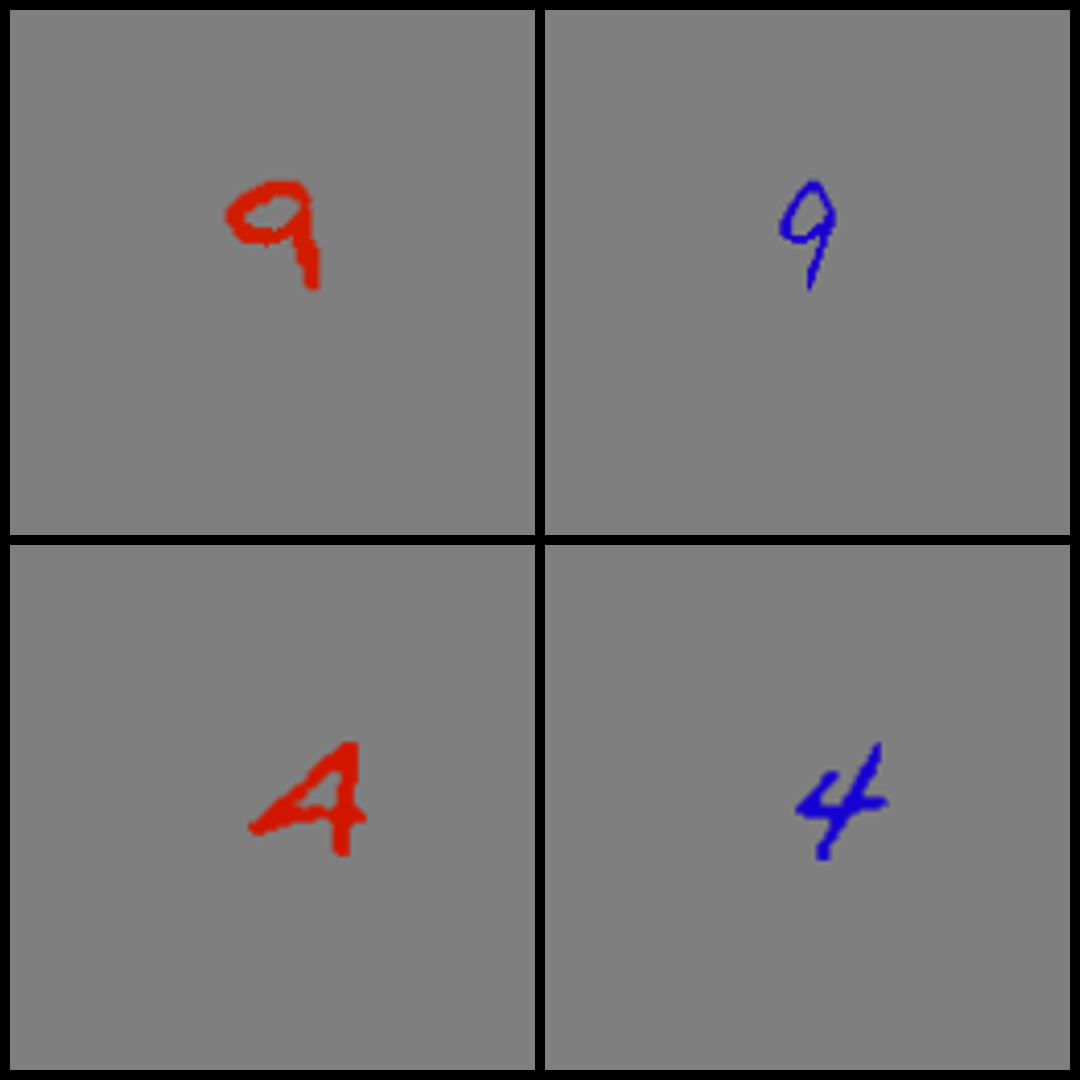
\includegraphics[height=2cm]{img/results_discussion/datashift/dsimages/train_collage.png}
        \caption*{Train}
    \end{subfigure}%
    \hfill
    \begin{subfigure}[b]{0.2\textwidth}
        \centering
        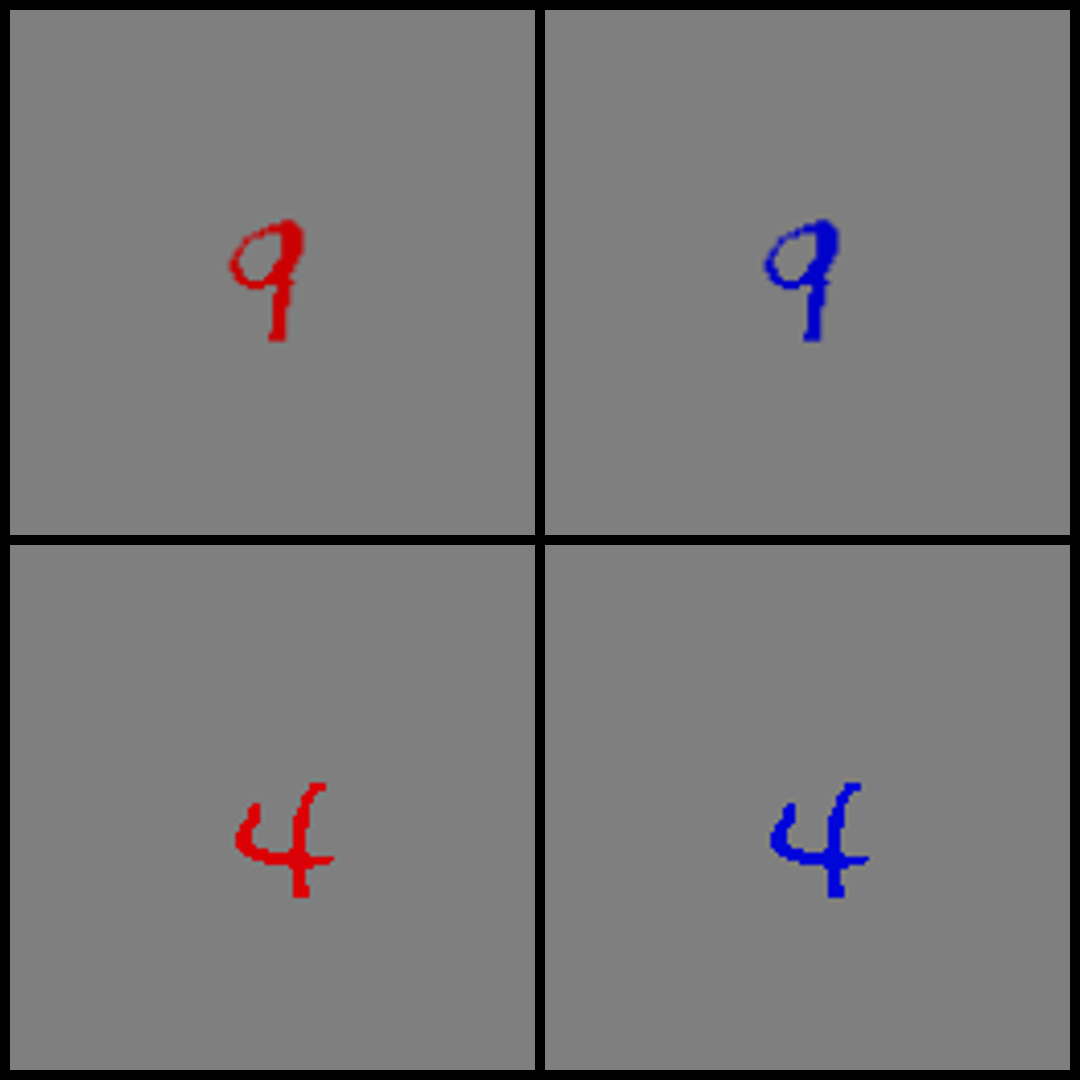
\includegraphics[height=2cm]{img/results_discussion/datashift/dsimages/val_collage.png}
        \caption*{Validation}
    \end{subfigure}%
    \hfill
    \begin{subfigure}[b]{0.6\textwidth}
        \centering
        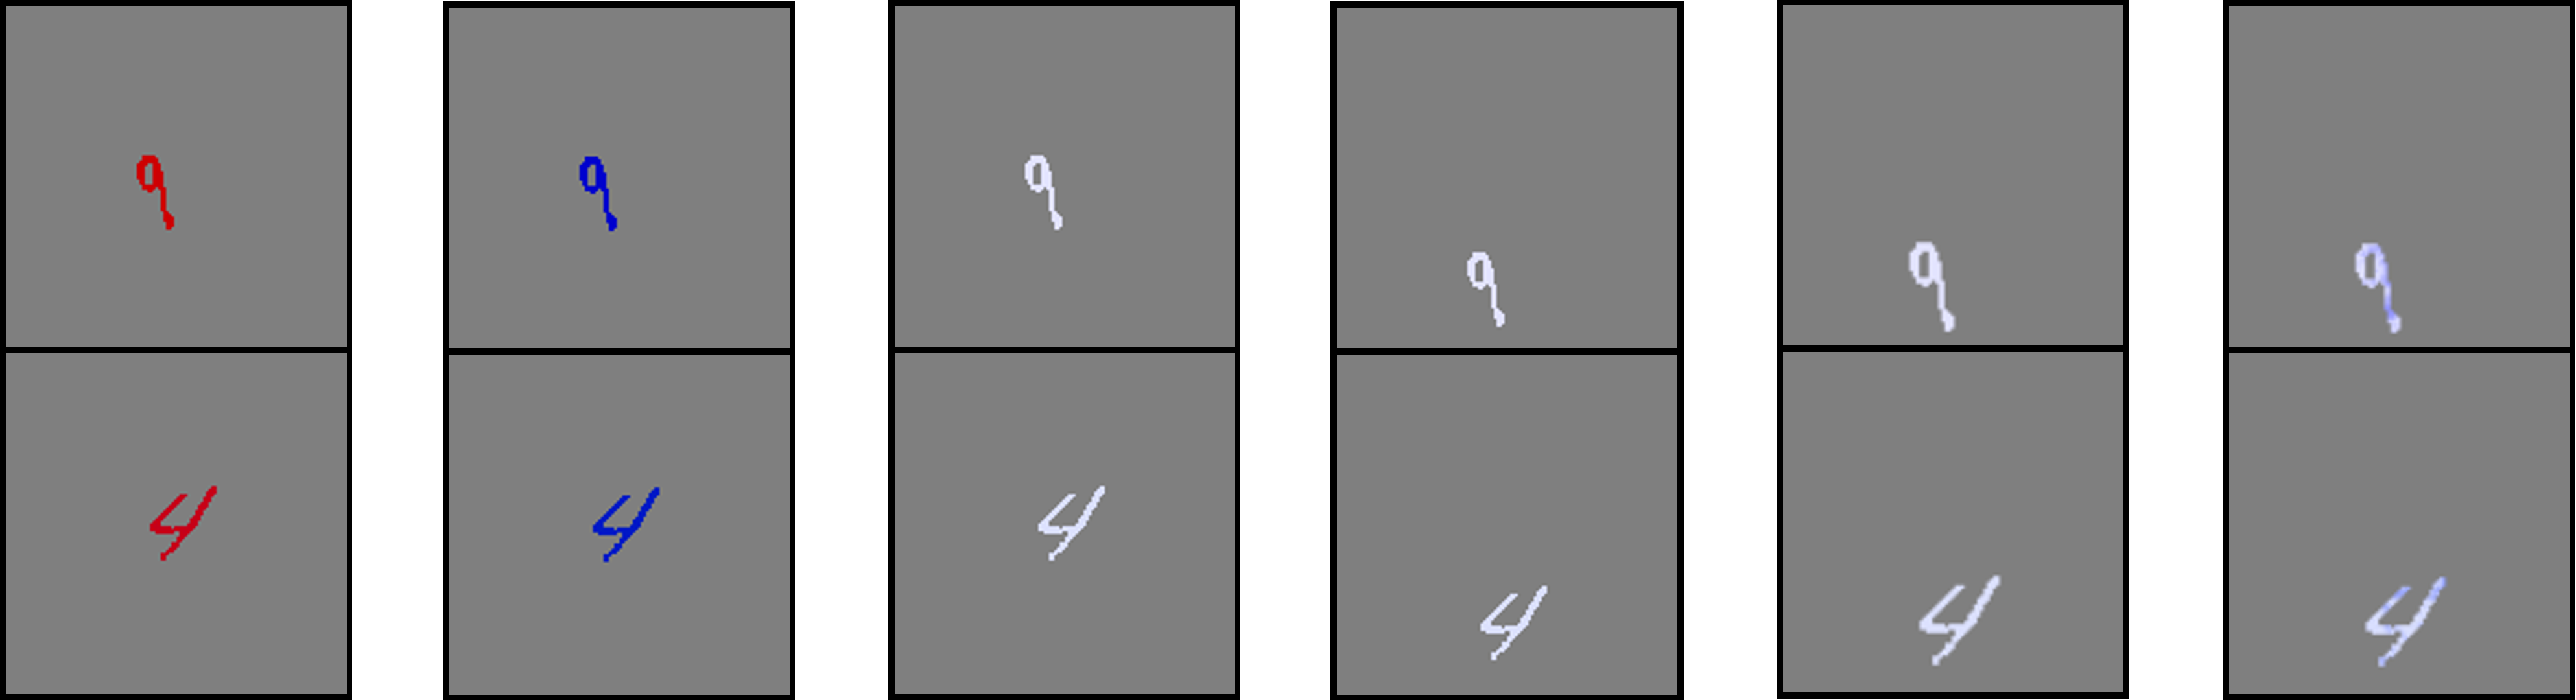
\includegraphics[height=2cm]{img/results_discussion/datashift/dsimages/test_collage2.png}
        \caption*{Test (0 - 5)}
    \end{subfigure}
    \caption{
    Illustration of the training, validation and test datasets. 
    Samples composing training datasets belong to different MNIST subsets, whereas samples composing
    validation and test datasets are corresponding (i.e. they are the same observation).
    }
    \label{fig:data_shift_images}
\end{figure}

ERM, IRM \cite{arjovskyInvariantRiskMinimization2020} and
LISA \cite{yaoImprovingOutofDistributionRobustness2022} algorithms were used to train a ResNet18 architecture
for 100 epochs on dataset $D^{\text{train}}$ using Adam \cite{kingmaAdamMethodStochastic2017}
optimizer with a learning rate 
of $10^{-3}$. Accuracy on validation dataset $D^{\text{val}}$ was monitored and weights
achieving maximum performance were selected for evaluation. The LISA interpolation
factor $p \in [0,1]$ was also selected following this criterion and was ultimately set to $0.5$, 
which indicates that both domain and factor interpolation between training samples
contribute to improve task performance in this setting. \\

Figure \ref{fig:pa_datashift_nonpaired} illustrates the discriminative capabilities of PA 
across test datasets. PA is shown to to decrease monotonically with increasing shift ratio and 
shift power in the cases of {\color{tab:blue} \textbf{Vanilla ERM}} and 
{\color{tab:orange} \textbf{Arjovsky et al.}}, with the latter being selected as a superior algorithm
under these conditions. In contrast, {\color{tab:green} \textbf{Yao et al.}}
does not exhibit the same consistent downward trend for $\alpha < 1$ and is notably penalized 
in the last dataset. This observation supports the robustness interpretation discussed in this work, suggesting that the model's 
inductive bias, rather than the data distribution, is responsible for this behavior. In particular, 
since LISA interpolates between observations from $\bm{x}_0^{\text{train}}$ and $\bm{x}_1^{\text{train}}$, 
the features encoded in the selected model may not align with those implicitly 
selected for the factor modification. \\

Table \ref{tab:shift_comparison_table_nonpaired} expands on this analysis
by providing the $\operatorname{AFR}_{\text{P}}$ and $\operatorname{AFR}_{\text{T}}$ scores
associated with this experiment for $\alpha=1$. PA assigns the highest score to {\color{tab:green} \textbf{Yao et al.}}
in the first dataset, which is composed from a configuration of factors that has been seen by the model
at training time, while consistently selecting {\color{tab:orange} \textbf{Arjovsky et al.}} as the 
most robust for the remaining cases. In contrast, accuracy-based metrics provide an 
inconsistent assessment across different levels of shift power that does not clearly discriminate
models by their response against source or target domain samples. In the absence of sampling randomness, 
a discontinuity in the feature representations that leads to this inconsistent behavior is not likely
to occur, especially when PA displays a consistent downward trend in most cases. \\

\begin{figure}[H]
    \centering
    \begin{subfigure}[b]{0.32\textwidth}
        \centering
        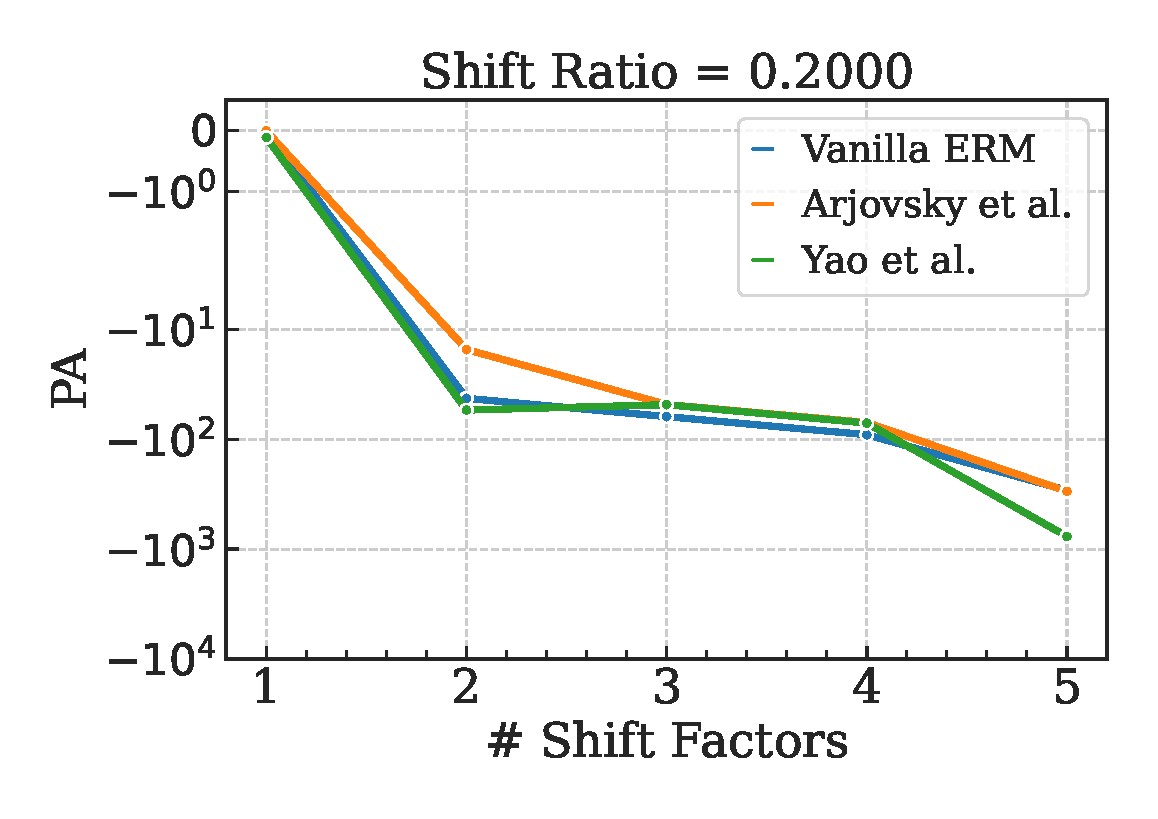
\includegraphics[width=\textwidth]{img/results_discussion/datashift/paper_nonpaired_sel=acc_met=PA_sr=0.2.pdf}
    \end{subfigure}
    \hfill
    \begin{subfigure}[b]{0.32\textwidth}
        \centering
        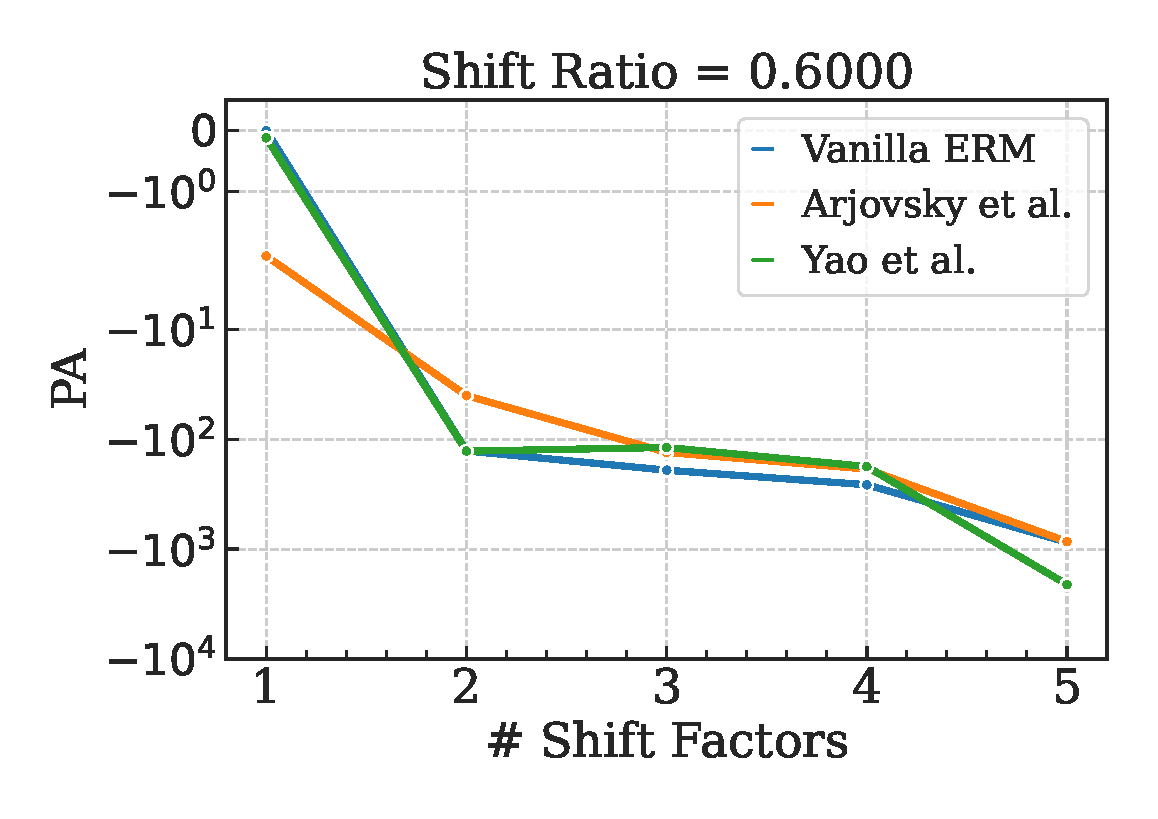
\includegraphics[width=\textwidth]{img/results_discussion/datashift/paper_nonpaired_sel=acc_met=PA_sr=0.6.pdf}
    \end{subfigure}
    \hfill
    \begin{subfigure}[b]{0.32\textwidth}
        \centering
        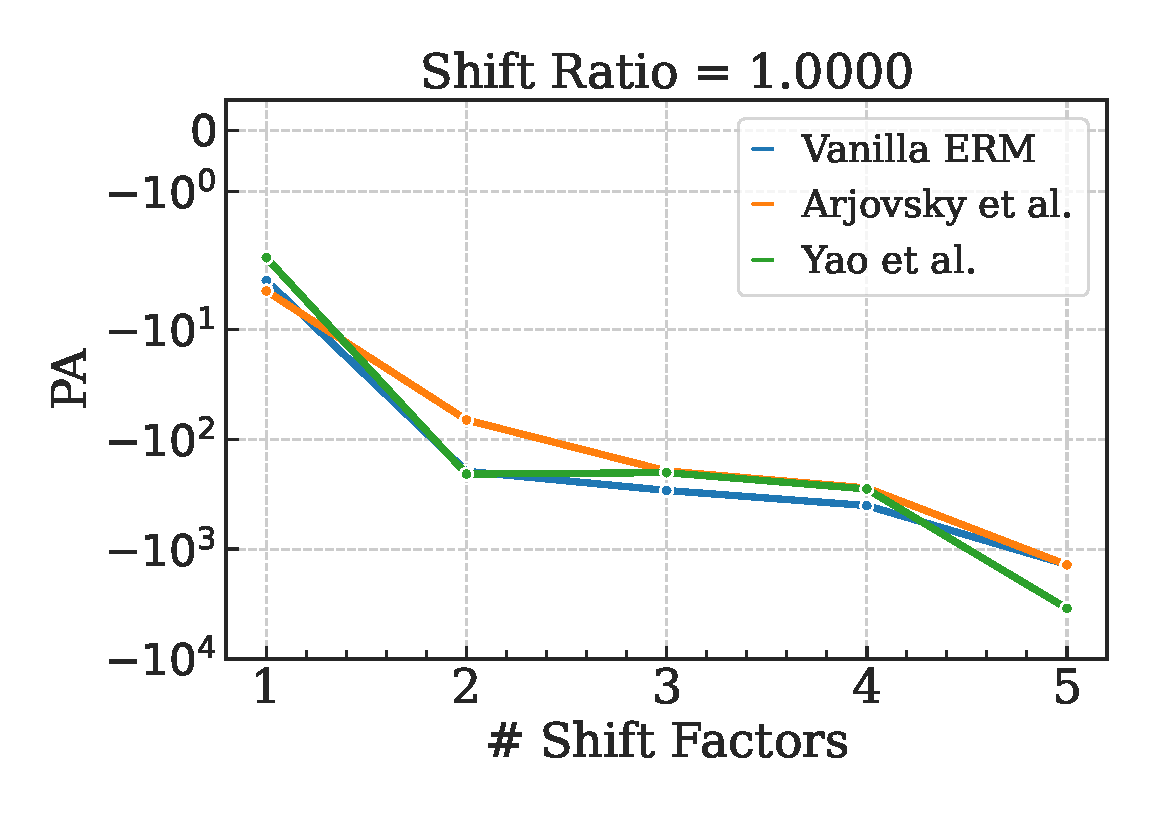
\includegraphics[width=\textwidth]{img/results_discussion/datashift/paper_nonpaired_sel=acc_met=PA_sr=1.0.pdf}
    \end{subfigure}

    \caption{
    Evolution of PA under increasing levels of shift power and shift ratio $\alpha$ for \textbf{Experiment 5a}. PA is sensitive to
    the domain from which samples are drawn (i.e. source for dataset 1, target for the rest) and provides
    a consistent assessment across increasing levels of domain shift and shift ratio. In particular, 
    {\color{tab:green} \textbf{Yao et al.}} achieves the highest score for the first dataset, whereas
    {\color{tab:orange} \textbf{Arjovsky et al.}} algorithm is considered the most robust for the remaining cases.
    }
    \label{fig:pa_datashift_nonpaired}
\end{figure}

\begin{table}[H]
    \centering
    \resizebox{\textwidth}{!}{%
    \begin{tabular}{l|ccc|ccc|ccc|ccc}
    \multirow{2}{*}{} & \multicolumn{3}{c|}{1 Shifted Factor} & \multicolumn{3}{c|}{2 Shifted Factors} & \multicolumn{3}{c|}{3 Shifted Factors} & \multicolumn{3}{c}{4 Shifted Factors}\\
     & PA & $\operatorname{AFR}_{\text{P}}$ & $\operatorname{AFR}_{\text{T}}$ & PA & $\operatorname{AFR}_{\text{P}}$  & $\operatorname{AFR}_{\text{T}}$ & PA & $\operatorname{AFR}_{\text{P}}$  & $\operatorname{AFR}_{\text{T}}$ & PA & $\operatorname{AFR}_{\text{P}}$  & $\operatorname{AFR}_{\text{T}}$ \\
    \midrule
    {\color{tab:blue} \textbf{Vanilla ERM}} & -3.583 & 0.999 & 0.992 & -195.4	& 0.979 & 0.973 & 291.8 & 0.968 & 0.963 & -400.9 & 0.957 & 0.953 \\
    {\color{tab:orange} \textbf{Arjovsky et al.}} & -4.463 & 0.999 & 0.989 & \textbf{-66.54} & \textbf{0.994} & 0.987 & \textbf{-194.2} & 0.982 & 0.978 & \textbf{-277.1} & 0.974 & \textbf{0.972} \\
    {\color{tab:green} \textbf{Yao et al.}} & \textbf{-2.219} & \textbf{0.999} & \textbf{0.993} & -207.2 & 0.980 & \textbf{0.975} & -200.9 & \textbf{0.983} & \textbf{0.979} & -282.9 & \textbf{0.976} & 0.970 \\
    \bottomrule
    \end{tabular}
    }
    \caption{
        Comparison of PA, $\operatorname{AFR}_{\text{P}}$ and $\operatorname{AFR}_{\text{T}}$ scores
        for ERM, IRM and LISA learning algorithms with $\alpha=1$ for \textbf{Experiment 5a}. The highest
        robustness score is emboldened for every case. PA provides a consistent assessment across target domains
        and selects {\color{tab:orange} \textbf{Arjovsky et al.}} as the most robust model. In contrast, accuracy-based
        metrics are less discriminative and significantly inconsistent across datasets, thus yielding no
        clear verdict.
    }
    \label{tab:shift_comparison_table_nonpaired}
\end{table}

\paragraph{Experiment 5b.} Alternative results were obtained by considering different sampling
instantiations $\tau_0^{\text{val}} \neq \tau_1^{\text{val}}$ and $\tau_0^{\text{test}} \neq \tau^{\text{test}}$ to 
generate the first validation and test datasets. In particular,

$$
D^{\text{val}} = \{\bm{x}_0^{\text{val}} \circ \tau_0^{\text{val}}, \bm{x}_1^{\text{val}} \circ \tau_1^{\text{val}}\} \;\; \text{and} \;\; D_0^{\text{test}} = \{ \bm{x}_0^{\text{test}} \circ \tau_0^{\text{test}} \}.
$$

In this variation of \textbf{Experiment 5a}, samples $\bm{x}_0^{\text{test}}$ and $\bm{x}_j^{\text{test}}$,
$j=\{1, \dots, 5\}$, are shifted due to both sampling randomness and image factor instantiations. This setting 
is not expected to change abruptly the performance score provided by accuracy-based metrics, but will definitely 
lower the PA robustness score, as the overlap between posteriors will decrease. \\

Figure \ref{fig:pa_datashift_nonpaired} shows that PA succeeds at discriminating the 
different models by their predictive response under increasing shift ratio and 
shift power. In particular, {\color{tab:blue} \textbf{Vanilla ERM}} can be identified 
to be non-robust by the fact that its score is maximum for the first test dataset, which belongs 
to the source domains, but decays rapidly to a minimum value after an additional factor is shifted. 
In contrast, {\color{tab:orange} \textbf{Arjovsky et al.}} and {\color{tab:green} \textbf{Yao et al.}} 
models display a lower robustness score for the first test dataset, especially
for small shift ratio values, but then decay at a lower rate than ERM
for the following target datasets. In this case, {\color{tab:green} \textbf{Yao et al.}} is 
selected as the most robust model through both performance-based and robustness-based metrics. This
change with respect to the previous experiment indicates that sample interpolation provides increased
robustness against sampling randomness. In the previous setting, where samples $\bm{x}_0^{\text{test}}$
and $\bm{x}_j^{\text{test}}$ were composed of the same MNIST observations, this advantage was not exploited and
the domain-invariance regularization performed by {\color{tab:orange} \textbf{Arjovsky et al.}} was shown to
be more effective. \\

These statements are further supported by the comparison of PA, $\operatorname{AFR}_{\text{P}}$ and
$\operatorname{AFR}_{\text{T}}$ scores in Table \ref{tab:shift_comparison_table}. The robustness assessment
provided by PA aligns with that of accuracy-based metrics in all target domains, which differs from the
behavior observed in the absence of sampling randomness (see Table \ref{tab:shift_comparison_table_nonpaired}). Nevertheless, only 
PA assigns the highest score to {\color{tab:blue} \textbf{Vanilla ERM}} on the first test dataset, which belongs to the source domain and thus
represents a combination of factors that the model has seen during training. This is a clear indication
that PA is able to capture the generalization capabilities of the model in a more substantial way than
accuracy-based metrics, which are unable to discriminate different test datasets. \\

Figure \ref{fig:pa_datashift_nonpaired} also shows an unexpected increase in PA after four 
shifted factors, which seems inconsistent with the alleged non-increasing behavior of PA, as per
Section \ref{sec:robustness_to_covariate_shift}. Nevertheless, this phenomenon 
highlights again that robustness does not stem from the data generation process but rather 
from the latent representation of the model and the features selected for the construction 
of its inductive bias, as discussed in the introducting chapter. In this particular case, 
Table \ref{tab:CS_shift} proves that
there is a clear discontinuity in the feature representation of the data when the texture
factor is shifted (see Table \ref{tab:data_shift_table}), which results in a different discriminator function that ultimately
leads to a different predictive outcome. \\


\begin{figure}[H]
    \centering
    \begin{subfigure}[b]{0.32\textwidth}
        \centering
        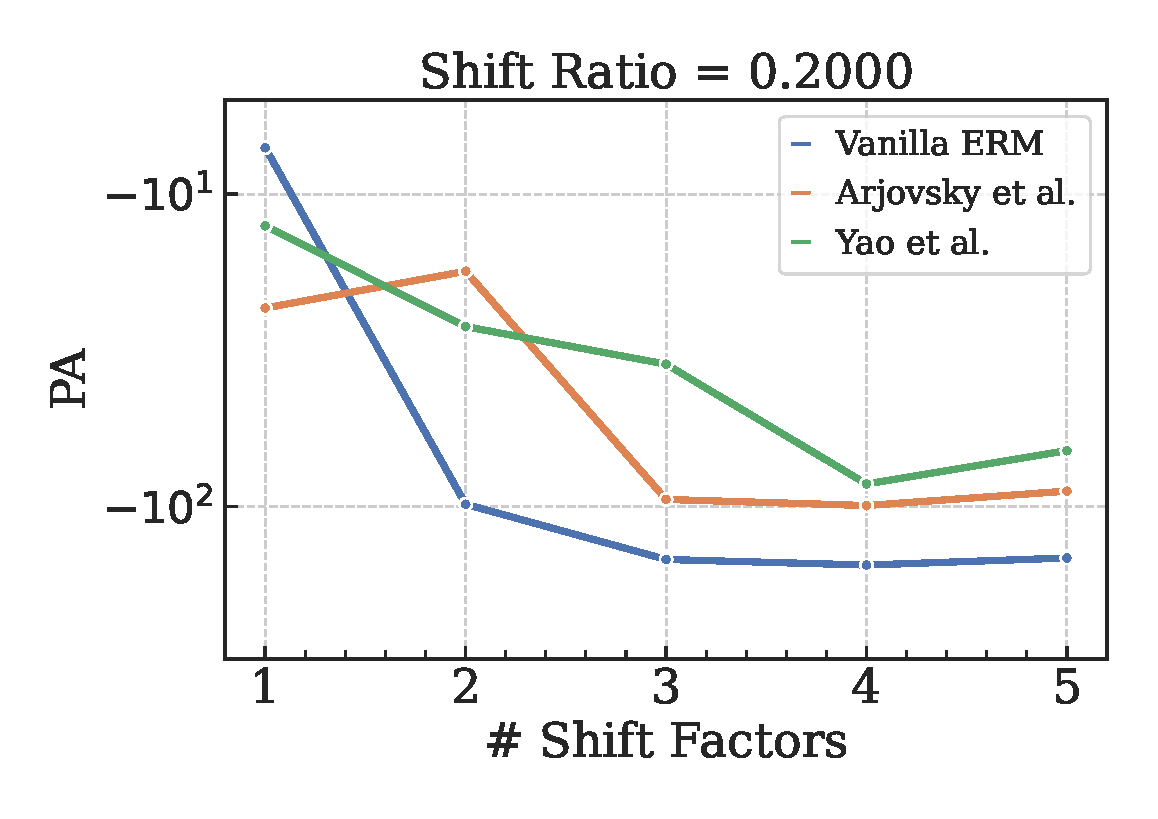
\includegraphics[width=\textwidth]{img/results_discussion/datashift/shift_ratio=0.200.pdf}
    \end{subfigure}
    \hfill
    \begin{subfigure}[b]{0.32\textwidth}
        \centering
        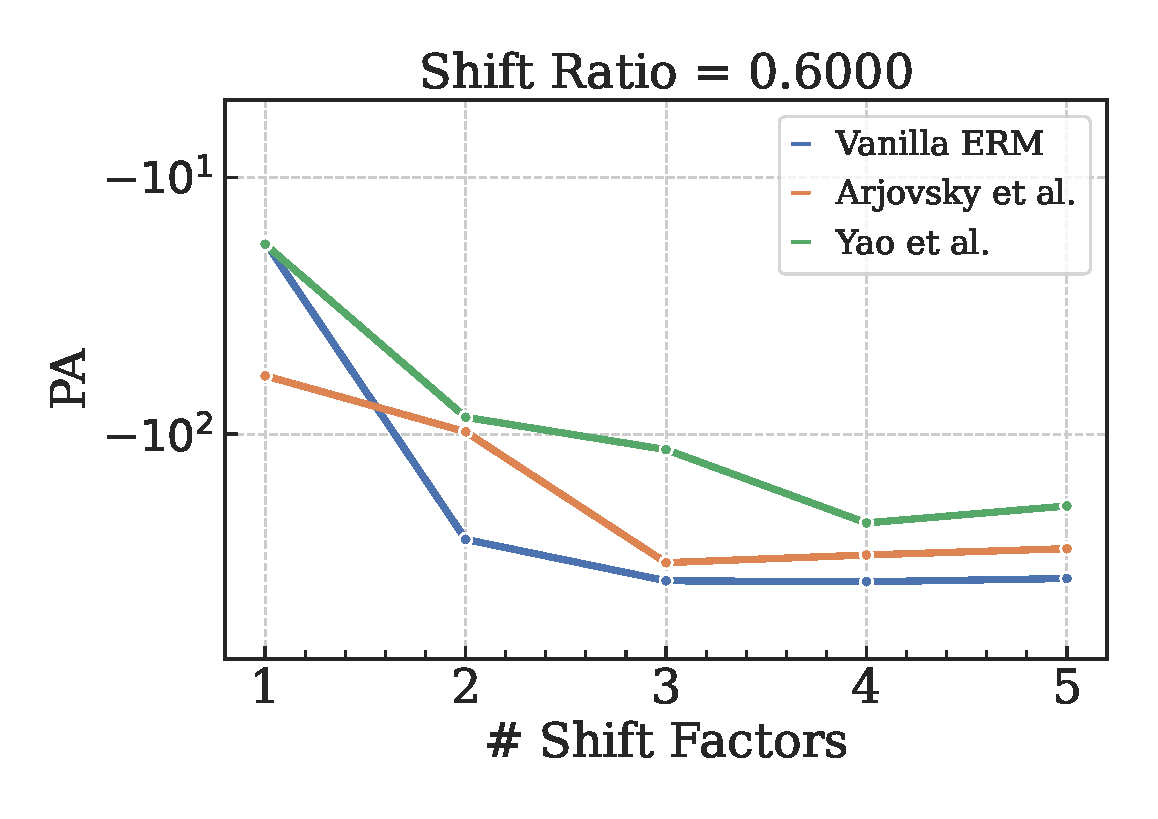
\includegraphics[width=\textwidth]{img/results_discussion/datashift/shift_ratio=0.600.pdf}
    \end{subfigure}
    \hfill
    \begin{subfigure}[b]{0.32\textwidth}
        \centering
        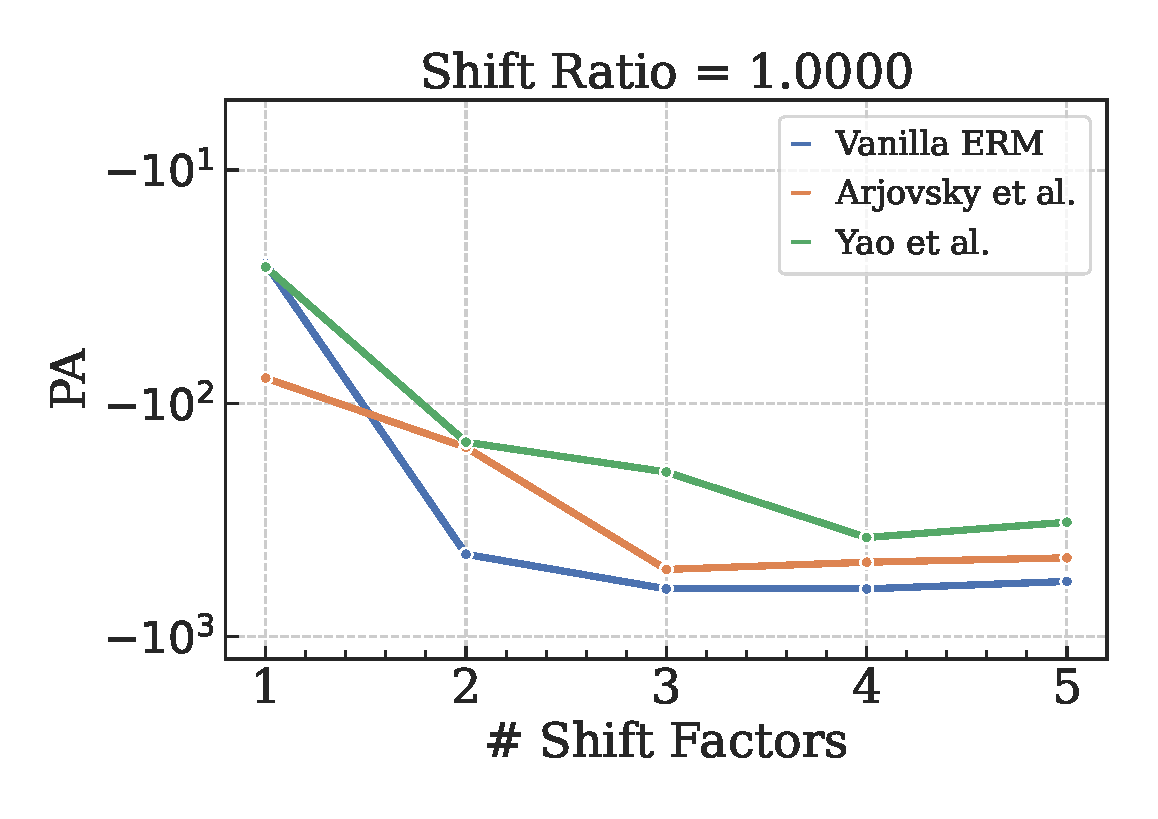
\includegraphics[width=\textwidth]{img/results_discussion/datashift/shift_ratio=1.000.pdf}
    \end{subfigure}

    % \vspace{1em}

    % \begin{subfigure}[b]{0.3\textwidth}
    %     \centering
    %     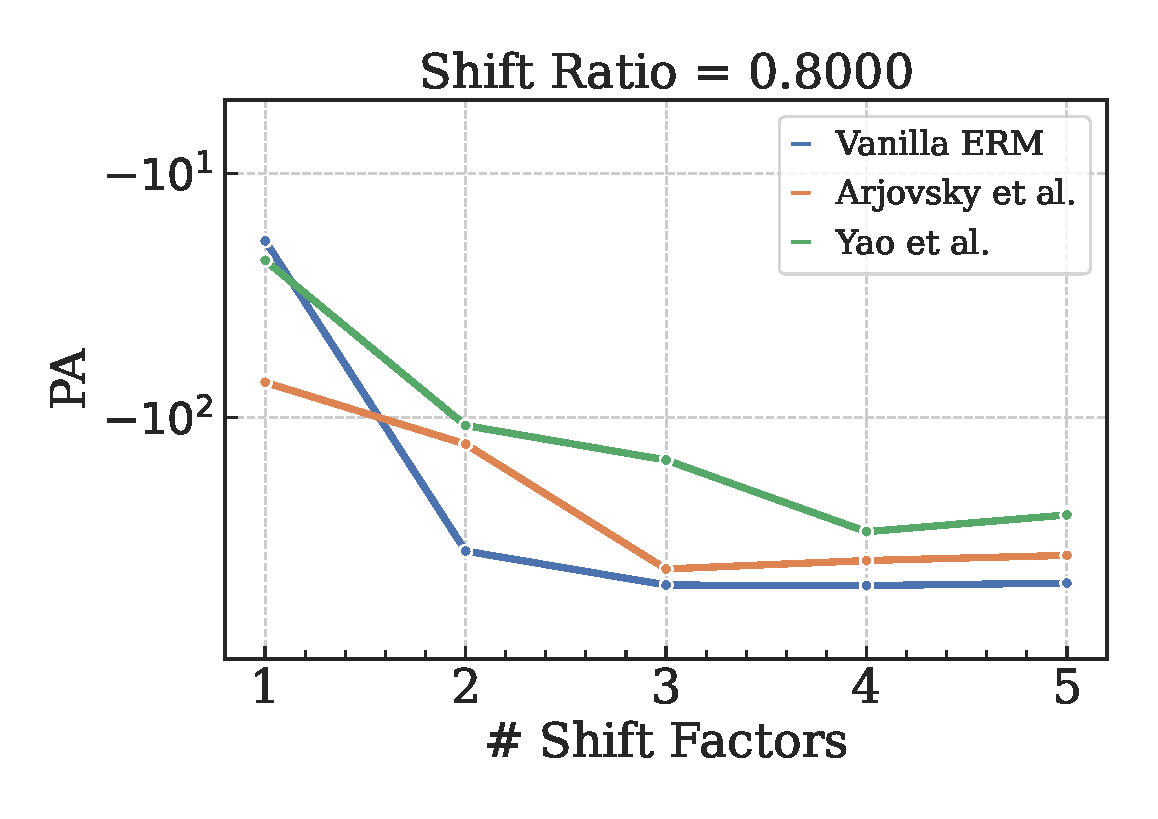
\includegraphics[width=\textwidth]{img/results_discussion/datashift/shift_ratio=0.800.pdf}
    % \end{subfigure}
    % \hspace{13pt}
    % \begin{subfigure}[b]{0.3\textwidth}
    %     \centering
    %     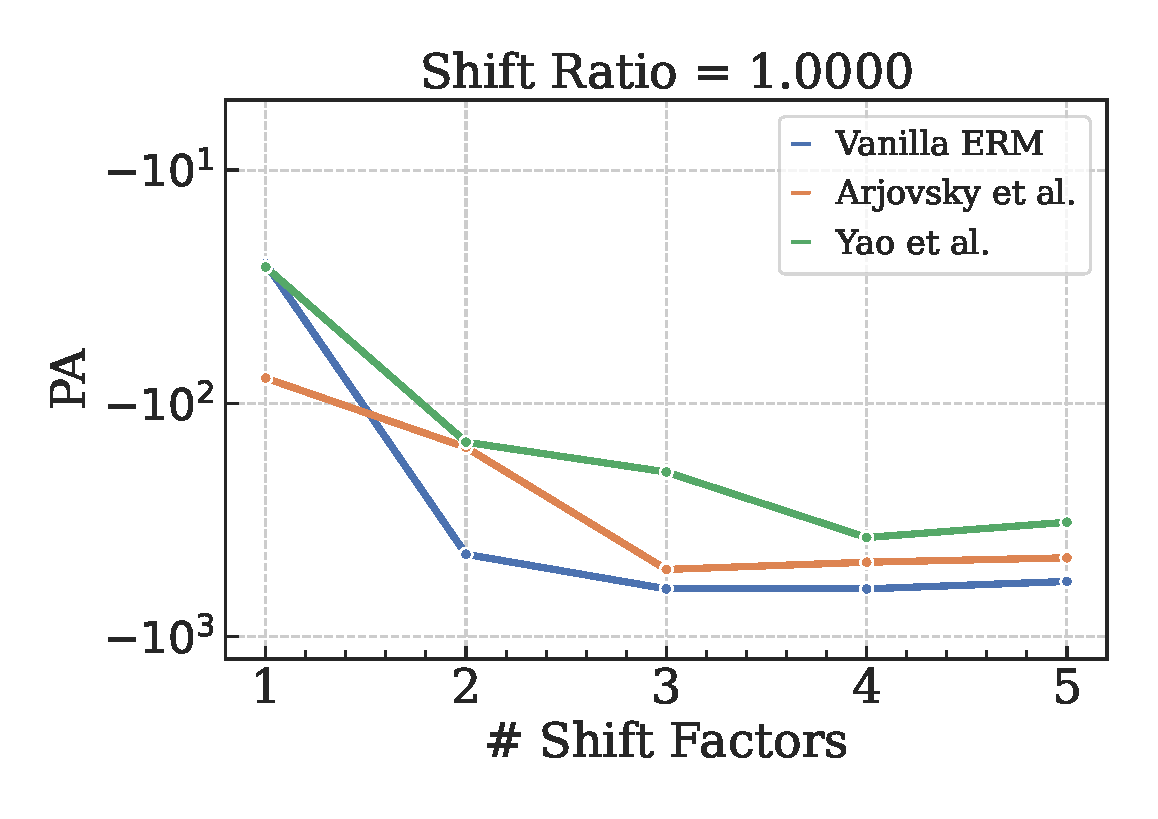
\includegraphics[width=\textwidth]{img/results_discussion/datashift/shift_ratio=1.000.pdf}
    % \end{subfigure}

    \caption{
    Evolution of PA under increasing levels of shift power and shift ratio $\alpha$ for \textbf{Experiment 5b}. Even in the presence of
    sampling randomness, PA is highly sensitive to source and domain environments and provides
    a consistent assessment of the generalization capabilities of the different models. }
    
    % In particular, the
    % {\color{tab:blue} \textbf{Vanilla ERM}} algorithm provides the best performance on the source, while
    % {\color{tab:green} \textbf{Yao et al.}} is selected as the most robust for the remaining cases.
    % }
    \label{fig:pa_datashift_paired}
\end{figure}

\begin{table}[H]
    \centering
    \resizebox{\textwidth}{!}{%
    \begin{tabular}{l|ccc|ccc|ccc}
    \multirow{2}{*}{} & \multicolumn{3}{c|}{1 Shifted Factor} & \multicolumn{3}{c|}{3 Shifted Factors} & \multicolumn{3}{c}{5 Shifted Factors} \\
     & PA & $\operatorname{AFR}_{\text{P}}$ & $\operatorname{AFR}_{\text{T}}$ & PA & $\operatorname{AFR}_{\text{P}}$  & $\operatorname{AFR}_{\text{T}}$ & PA & $\operatorname{AFR}_{\text{P}}$  & $\operatorname{AFR}_{\text{T}}$ \\
    \midrule
    {\color{tab:blue} \textbf{Vanilla ERM}} & \textbf{-24.91}  & 0.999 & 0.993 & -625.6 & 0.979 & 0.975 & -579.4 & 0.976 & 0.873 \\
    {\color{tab:orange} \textbf{Arjovsky et al.}} & -76.76 & 0.998 & 0.993 & -514.2 & 0.976 & 0.978  & -464.2 & 0.976 & 0.911 \\
    {\color{tab:green} \textbf{Yao et al.}} & -26.21 & \textbf{0.999} & \textbf{0.994} & \textbf{-201.2} & \textbf{0.985} & \textbf{0.980} & \textbf{-324.4} & \textbf{0.988} & \textbf{0.945} \\
    \bottomrule
    \end{tabular}
    }
    \caption{
        Comparison of PA, $\operatorname{AFR}_{\text{P}}$ and $\operatorname{AFR}_{\text{T}}$ scores
        for ERM, IRM and LISA learning algorithms with $\alpha=1$ for \textbf{Experiment 5b}. The 
        highest robustness score is emboldened for every case. PA is 
        able to discriminate algorithms consistently and distinguish
        the first shifted factor dataset, which is drawn from source domains, from the rest.
    }
    \label{tab:shift_comparison_table}
\end{table}



\begin{table}[H]
    \centering
    \begin{tabular}{l|c|c|c|c|c}
    \# Shift Factors & 1 & 2 & 3 & 4 & 5 \\
    \midrule
    {\color{tab:blue} \textbf{Vanilla ERM}} & 0.9978 & 0.9303 & 0.9562 & 0.9561 & \textbf{0.6661} \\
    {\color{tab:orange} \textbf{Arjovsky et al.}} & 0.9967 & 0.9018 & 0.9296 & 0.9374 & \textbf{0.5585} \\
    {\color{tab:green} \textbf{Yao et al.}}  & 0.9980 & 0.9431 & 0.9431 & 0.9641 & \textbf{0.7130} \\
    \bottomrule
    \end{tabular}
    \caption{
    Average pairwise cosine similarity between feature space representations of original and
    augmented images (i.e. $\bm{x}_0^{\text{test}}$ vs. $\bm{x}_j^{\text{test}}$), for each of the shifted datasets in \textbf{Experiment 5b}. The abrupt decrease in similarity
    for the fifth environment indicates a discontinuity in the feature representation of images,
    which leads to non-comparable predictive outcomes.
    }
    \label{tab:CS_shift}
    \end{table}

Finally, Figure \ref{fig:pa_datashift_posteriors} and Table \ref{tab:datashift_betas} display the average posterior
probability assigned to the predicted class for $\beta=1$, and the subsequent optimal $\beta^{*}$ value
derived from the maximization of posterior agreement, respectively. These results, which are reported for both
\textbf{Experiment 5a} and \textbf{Experiment 5b}, give insight into the rationale behind the assessment provided 
by PA. In particular, given that accuracy was not discriminative across models and $\bm{x}_0^{\text{test}}$, 
$\bm{x}_j^{\text{test}}$ displayed a similar number of matching observations for all $j \in \{1, \dots, 5\}$,
models providing the highest posterior probability to the correct class were selected as the most robust. \\

It follows also from the values of $\beta^{*}$ in Table \ref{tab:datashift_betas} that the presence of sampling 
randomness between datasets under consideration does not significantly alter the robustness assessment provided
in the {\color{tab:blue} \textbf{Vanilla ERM}} and {\color{tab:orange} \textbf{Arjovsky et al.}} cases, which indicates
that the inductive bias of these models generalizes to different instantiations of MNIST. In contrast, the 
{\color{tab:green} \textbf{Yao et al.}} model displays a different generalization performance in between
both experiments that does not stem from a difference in performance or $\operatorname{AFR}_{\text{P}}$. This 
suggests that PA can provide a more informative assessment of the generalization capabilities of models
and the suitability of the inductive bias of models under different conditions. In this particular case, the
features learned by {\color{tab:green} \textbf{Yao et al.}} yield poorly informative posteriors in the absence of
sampling randomness, which translates to a suboptimal robustness score in \textbf{Experiment 5a}. \\


\begin{figure}[H]
    \centering
    \begin{subfigure}[b]{0.48\textwidth}
        \centering
        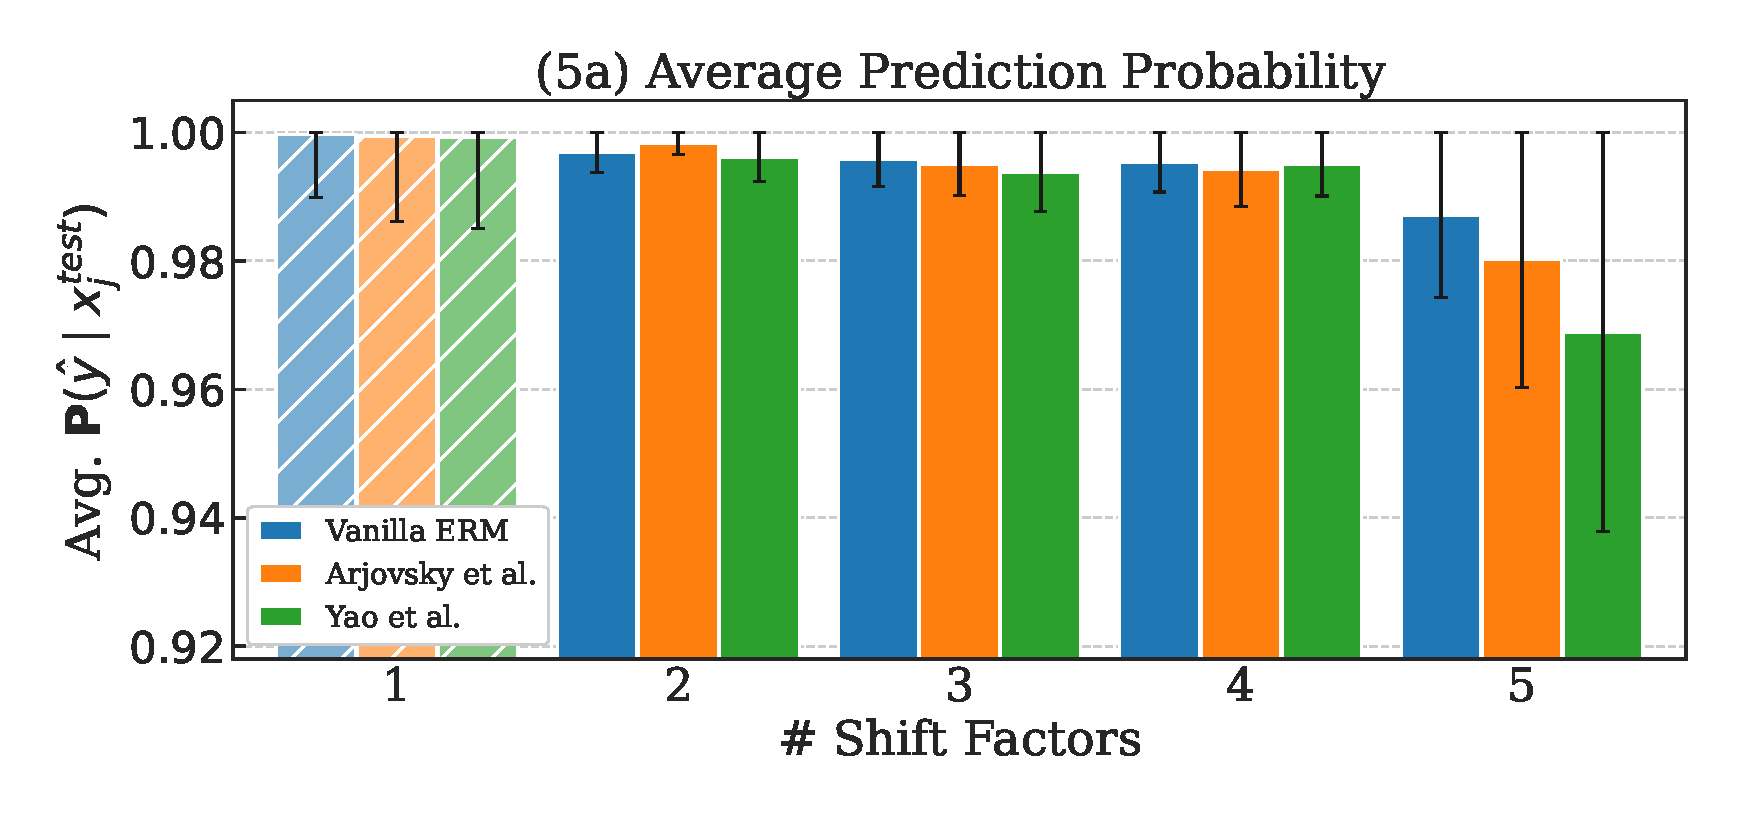
\includegraphics[width=\textwidth]{img/results_discussion/datashift/posterior_paper_nonpaired.pdf}
    \end{subfigure}
    \hfill
    \begin{subfigure}[b]{0.48\textwidth}
        \centering
        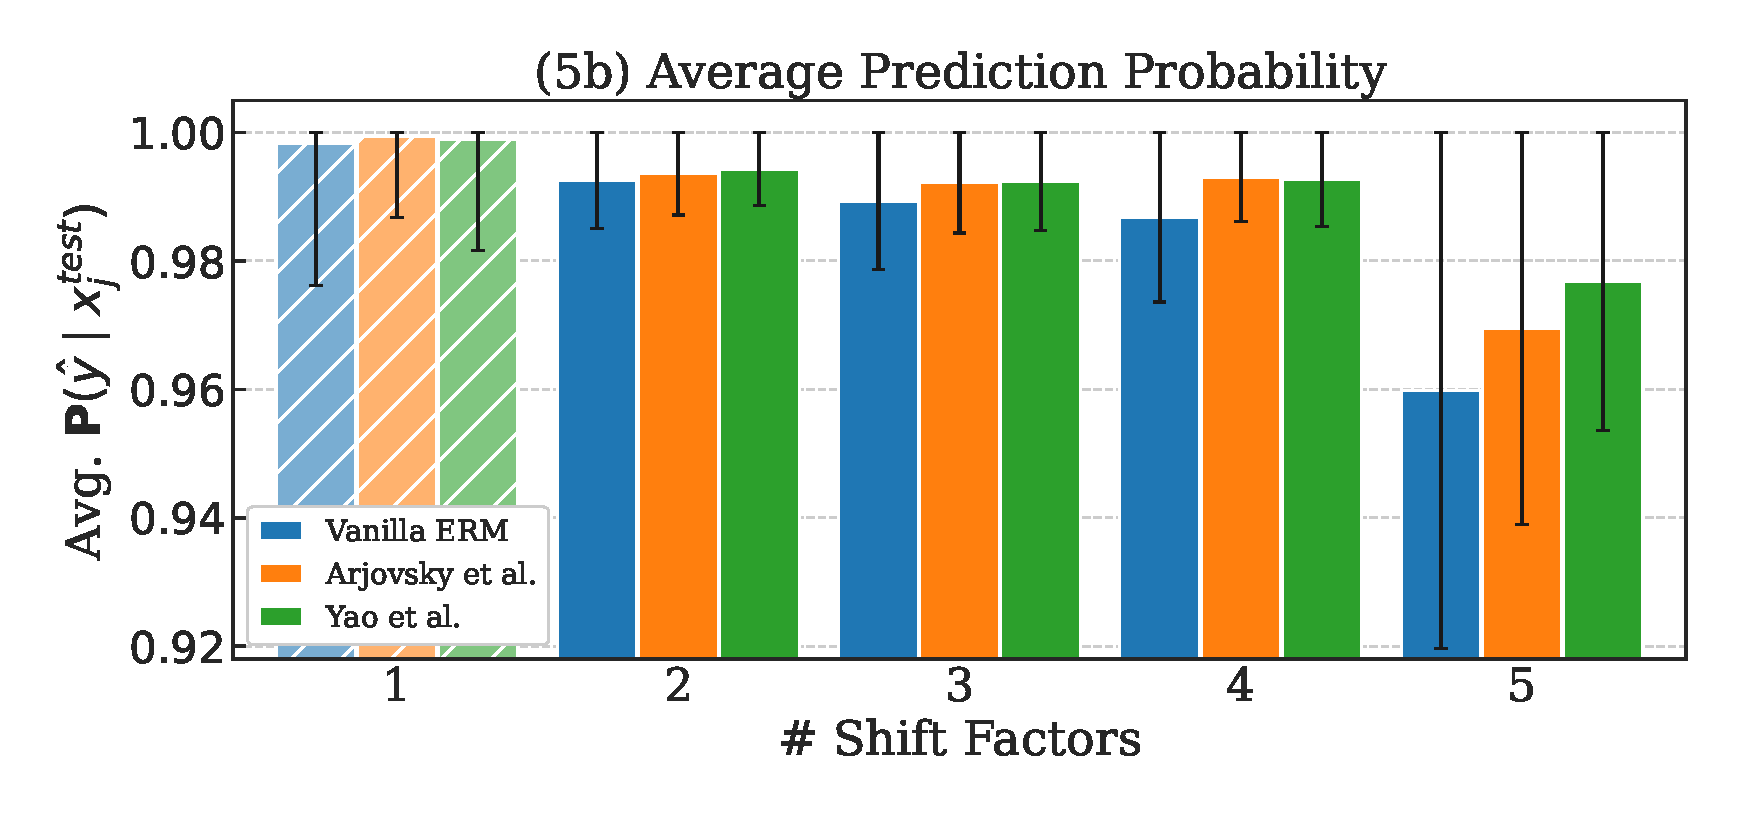
\includegraphics[width=\textwidth]{img/results_discussion/datashift/posterior_paper.pdf}
    \end{subfigure}

    \caption{
    Average posterior probability of the predicted class for each of the test datasets, under the conditions
    established for \textbf{Experiment 5a} (left) and \textbf{Experiment 5b} (right). The first dataset
    is distinguished from the rest for belonging to the source domains.
    }
    \label{fig:pa_datashift_posteriors}
\end{figure}

\begin{table}[H]
    \centering
    \begin{tabular}{l|c|c}
     & \textbf{Experiment 5a} & \textbf{Experiment 5b}\\
    \midrule
    \textbf{{\color{tab:blue} \textbf{Vanilla ERM}}} & 2.303  & 3.022   \\
    \textbf{{\color{tab:orange} \textbf{Arjovsky et al.}}} & 4.927  & 3.138  \\
    \textbf{{\color{tab:green} \textbf{Yao et al.}}} & 5.687 & 1.837 \\
    \bottomrule
    \end{tabular}
    \caption{
        Comparison of $\beta^{*}$ obtained after 1000 optimization epochs for both experiments 
        conducted in the out-of-distribution setting. Given that performance in source domains is
        almost identical across models, the informativeness of the predictions is the main driver
        of the robustness assessment provided by PA.
    }
    \label{tab:datashift_betas}
\end{table}

Overall, these results highlight that posterior agreement possesses a superior discriminative power
with respect to accuracy-based metrics. In particular, it provides a consistent assessment of the
generalization capabilities of models under different sources of randomness, as it has shown to be
sensitive to the presence of both sampling randomness and covariate shift and also to the type of 
domain (i.e. source or target) from which samples are drawn. This increased sensitivity is useful 
for the characterization and evaluation of inductive biases, which has been proven to 
determine the robust or unrobust behavior of models under different conditions. \\

The results obtained in this section further corroborate that all sources of randomness
that affect the data generation process are accounted for in the PA score. In the adversarial
setting, an approximation was performed so to discriminate the contribution of adversarial perturbations to
the overall robustness measure. In this setting, a different procedure will be followed that will separately
assess the suitability of the inductive bias against both distribution shift and sampling randomness. \\

\paragraph{Experiment 5c.}
    ERM and IRM \cite{arjovskyInvariantRiskMinimization2020} algorithms were used to train a ResNet18 model 
    for 50 epochs on dataset $D^{\text{train}}$ using Adam \cite{kingmaAdamMethodStochastic2017}
    optimizer with a learning rate of $10^{-2}$. A small subset of 128 observations from each 
    validation sample $\bm{x}_0^{\text{val}}$, $\bm{x}_1^{\text{val}}$
    generated for \textbf{Experiment 5a} is selected to generate a reduced validation dataset 
    $D^{\text{sub}} = \{ \bm{x}_0^{\text{sub}}, \bm{x}_1^{\text{sub}}\} \subset D^{\text{val}}$. Samples $\bm{x}_0^{\text{sub}}$, 
    $\bm{x}_1^{\text{sub}}$ entail the same randomness instantiation $\tau^{\text{val}}$ and therefore 
    are composed of the same MNIST observations and in the same order. Consequently, they are only
    subject to distribution shift, which in this case stems from the hue factor (i.e. blue vs red), 
    as per Table \ref{tab:data_shift_table}. \\

    At the end of every epoch, the principal component (see PCA \cite{jolliffe2002principal}) of the feature 
    space representation of $\bm{x}_0^{\text{sub}}$ and $\bm{x}_1^{\text{sub}}$ is computed separately, 
    so that each MNIST observation in $D^{\text{sub}}$ can be associated with two values, one obtained under each sample.
    In a qualitative way, the suitability of the inductive bias represented in a particular 
    epoch can be assessed by characterizing the principal component, which is the direction along 
    which the data exhibits the highest variance. \\

    Let $\Phi^c$ be the feature extractor of classifier $c$ after a training epoch. The principal
    direction of the feature space representations of samples $\bm{x}_0^{\text{sub}}$, $\bm{x}_1^{\text{sub}}$
    will be denoted as $\bm{v}_0$, $\bm{v}_1$, respectively. The projections of each observation over these
    components were computed as

    $$
    z_{0, n} = \langle \Phi^c(x_{0, n}^{\text{sub}}), \bm{v}_0 \rangle, \;\;\; z_{1, n} = \langle \Phi^c(x_{1, n}^{\text{sub}}), \bm{v}_1 \rangle , \;\; n = 1, \dots N_{\text{sub}}
    $$

    On the one hand, the distribution of observations belonging to different classes across the principal
    direction is an indicator of the task-specific suitability of the inductive bias. In general, the
    inductive bias of the model should be constructed with the most predictive features for the task at hand, 
    and therefore class membership should be the main driver of the variance in the feature space and thus 
    be encoded in the principal component. The class-conditional variance of $\bm{z}_0$, $\bm{z}_1$
    can be used as measure of the discriminative power of the latent features encoded, and consequently of the 
    robustness of the model against sampling randomness. \\
    
    On the other hand, the similarity between the projections of each observation along the principal direction 
    is an indicator of cross-domain invariance and consequently of the robustness of the model against 
    distribution shifts. If the inductive bias of the classifier were completely domain-agnostic, the 
    feature representations of shifted observations would be the same, and so its projection along the principal 
    direction. The mean squared error between the $\bm{z}_0$ and $\bm{z}_1$ can be used as a measure of
    the shift's influence in the inductive bias. \\


\begin{figure}[H]
    \centering
    \begin{subfigure}[b]{0.32\textwidth}
        \centering
        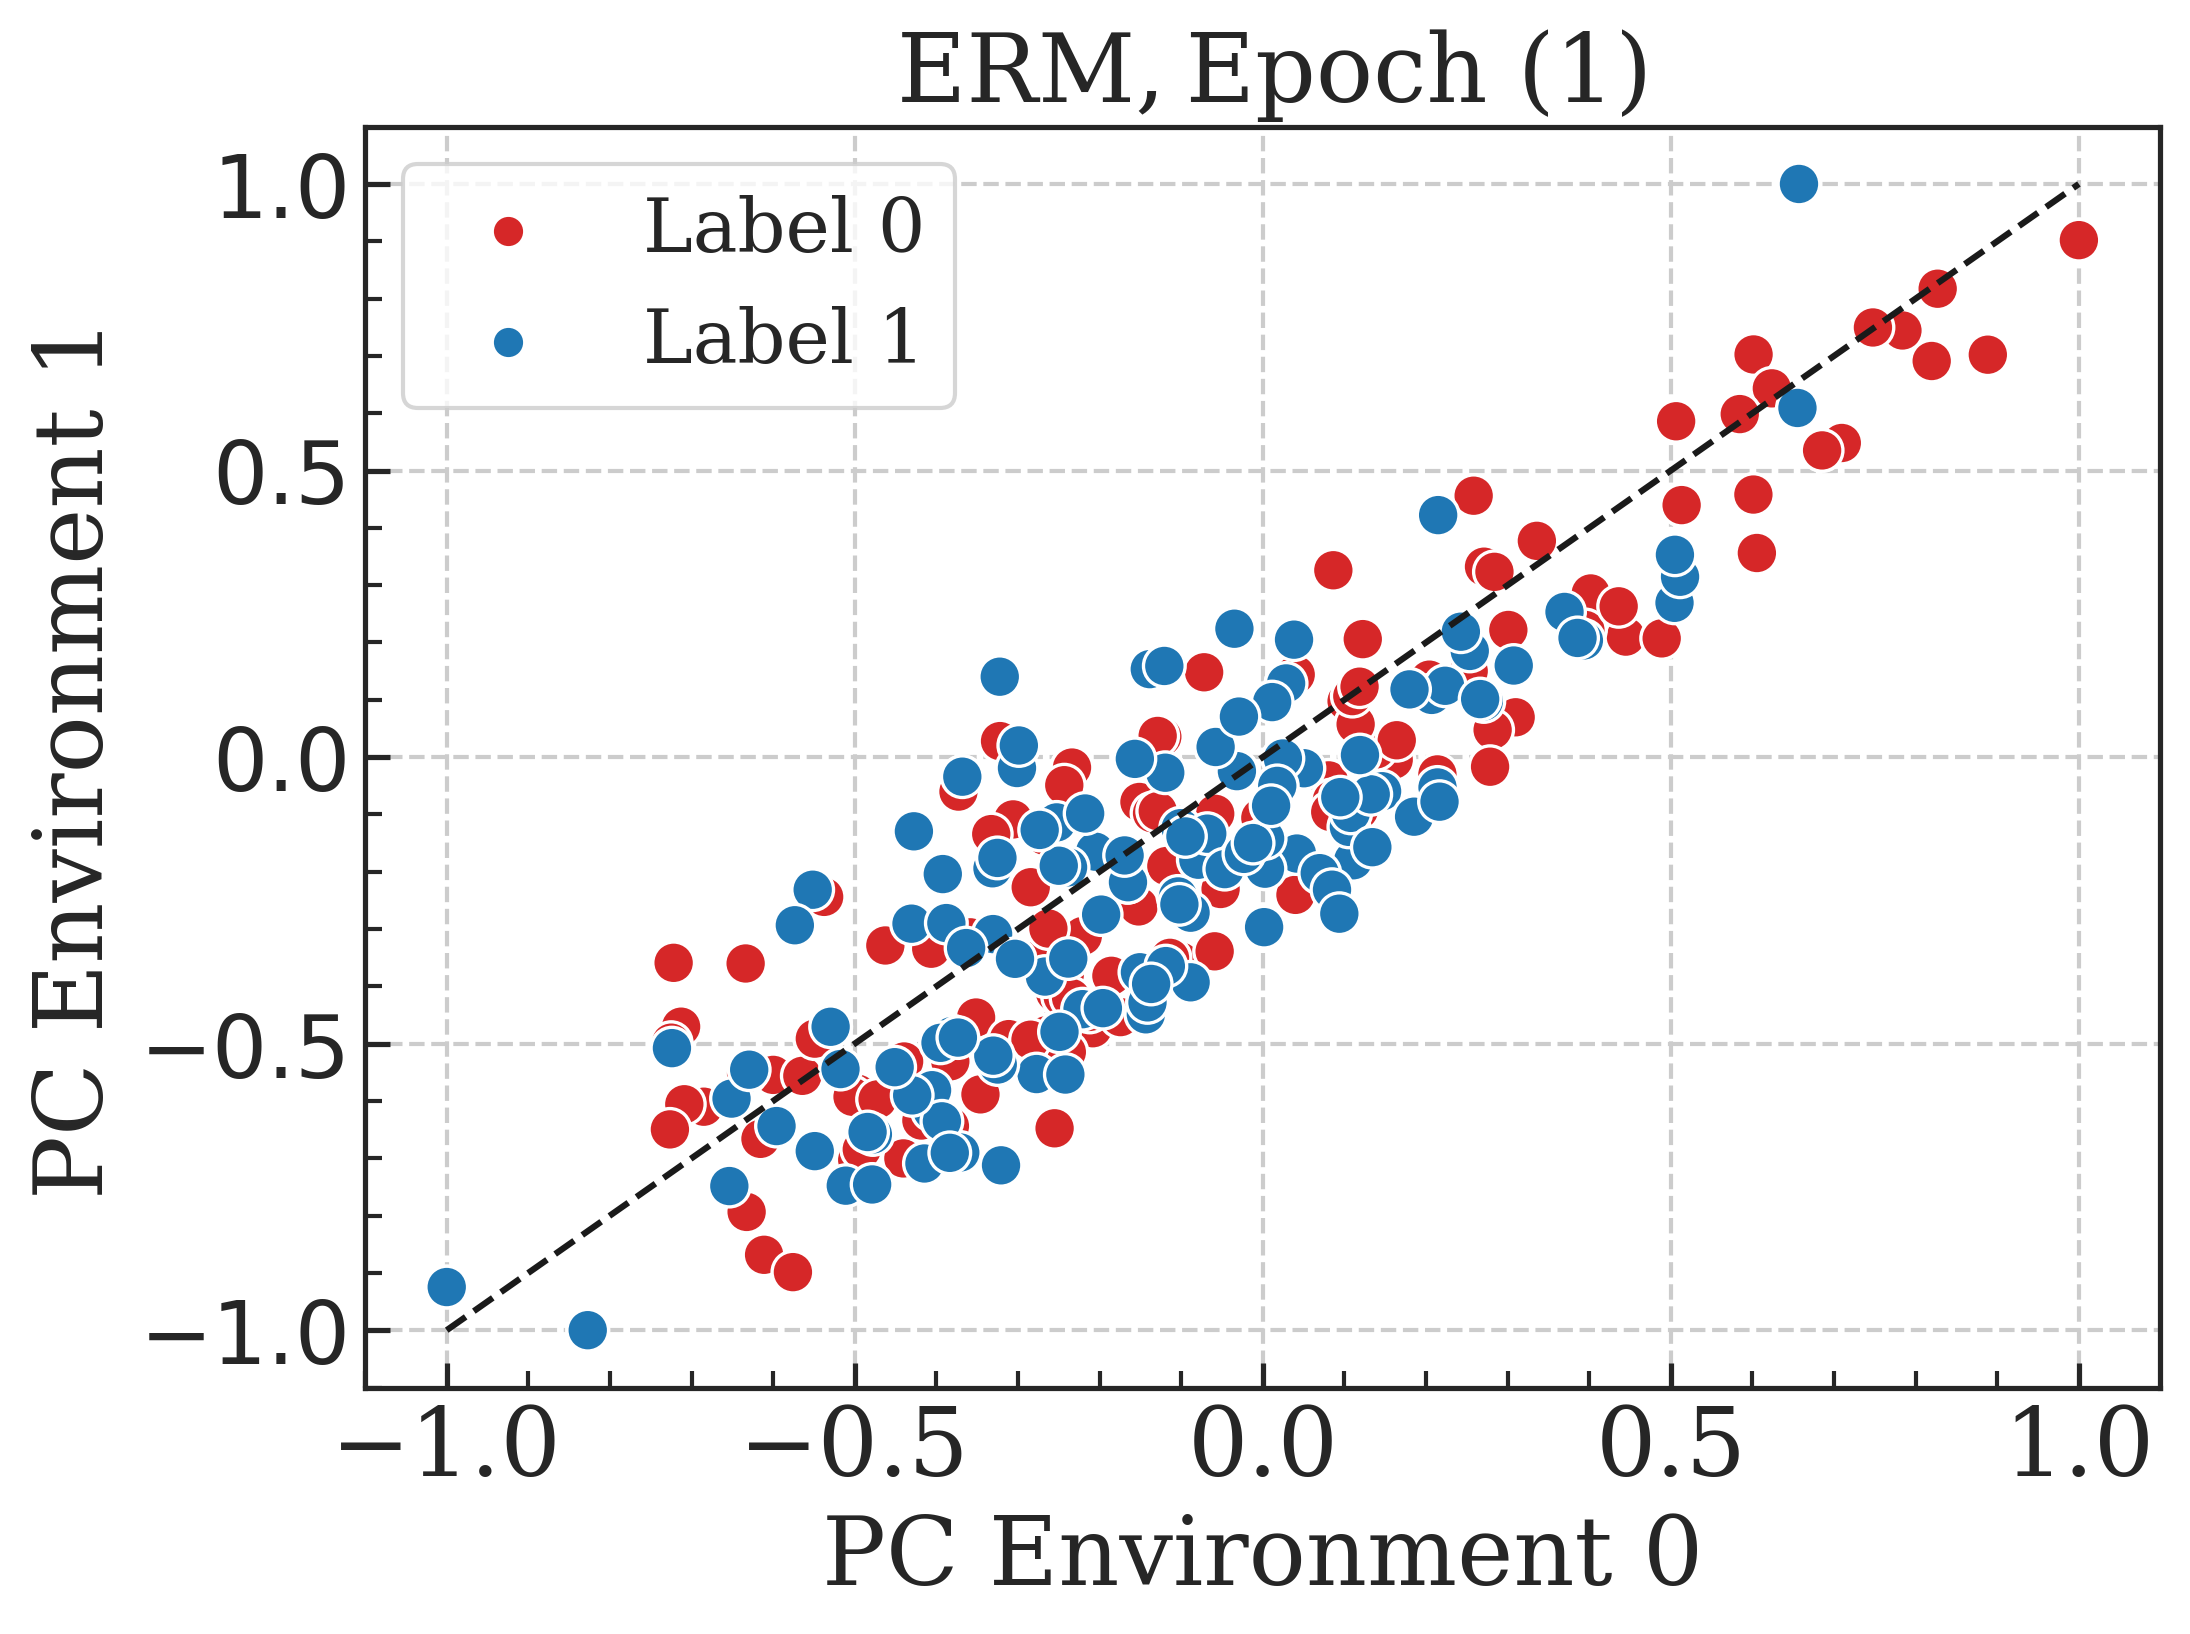
\includegraphics[width=\textwidth]{img/results_discussion/datashift/NL_1.png}
    \end{subfigure}
    \hfill
    \begin{subfigure}[b]{0.32\textwidth}
        \centering
        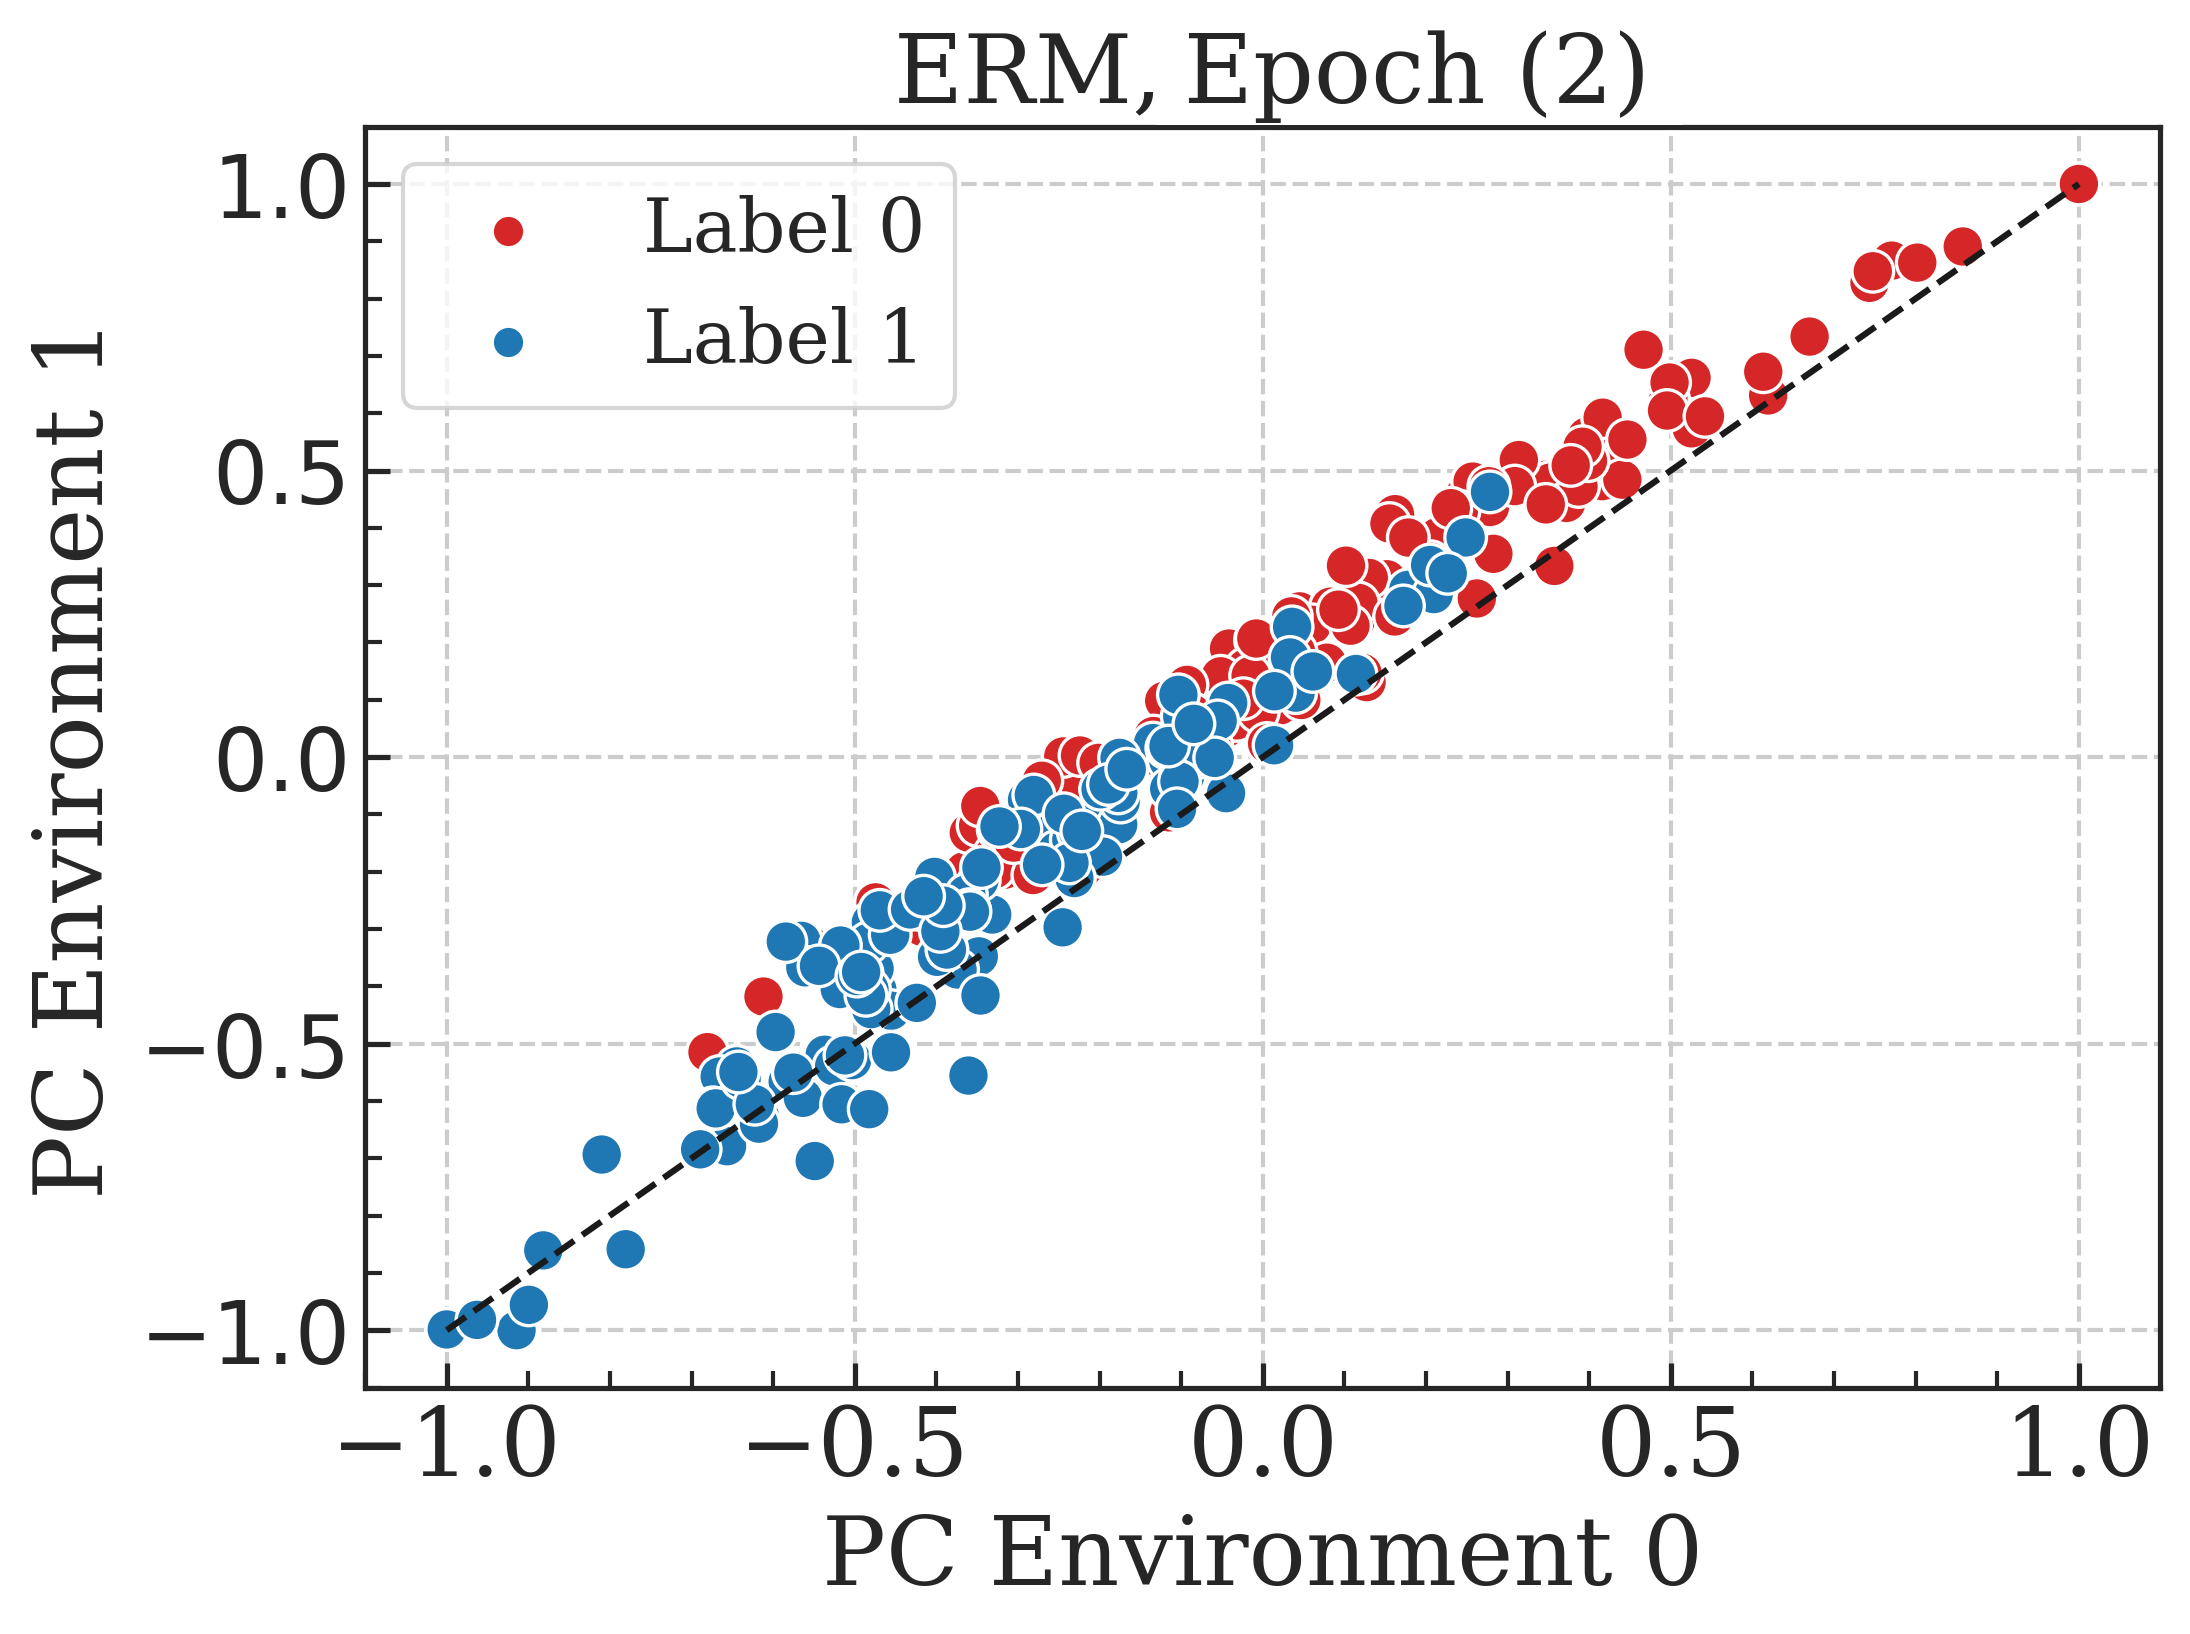
\includegraphics[width=\textwidth]{img/results_discussion/datashift/NL_2.png}
    \end{subfigure}
    \hfill
    \begin{subfigure}[b]{0.32\textwidth}
        \centering
        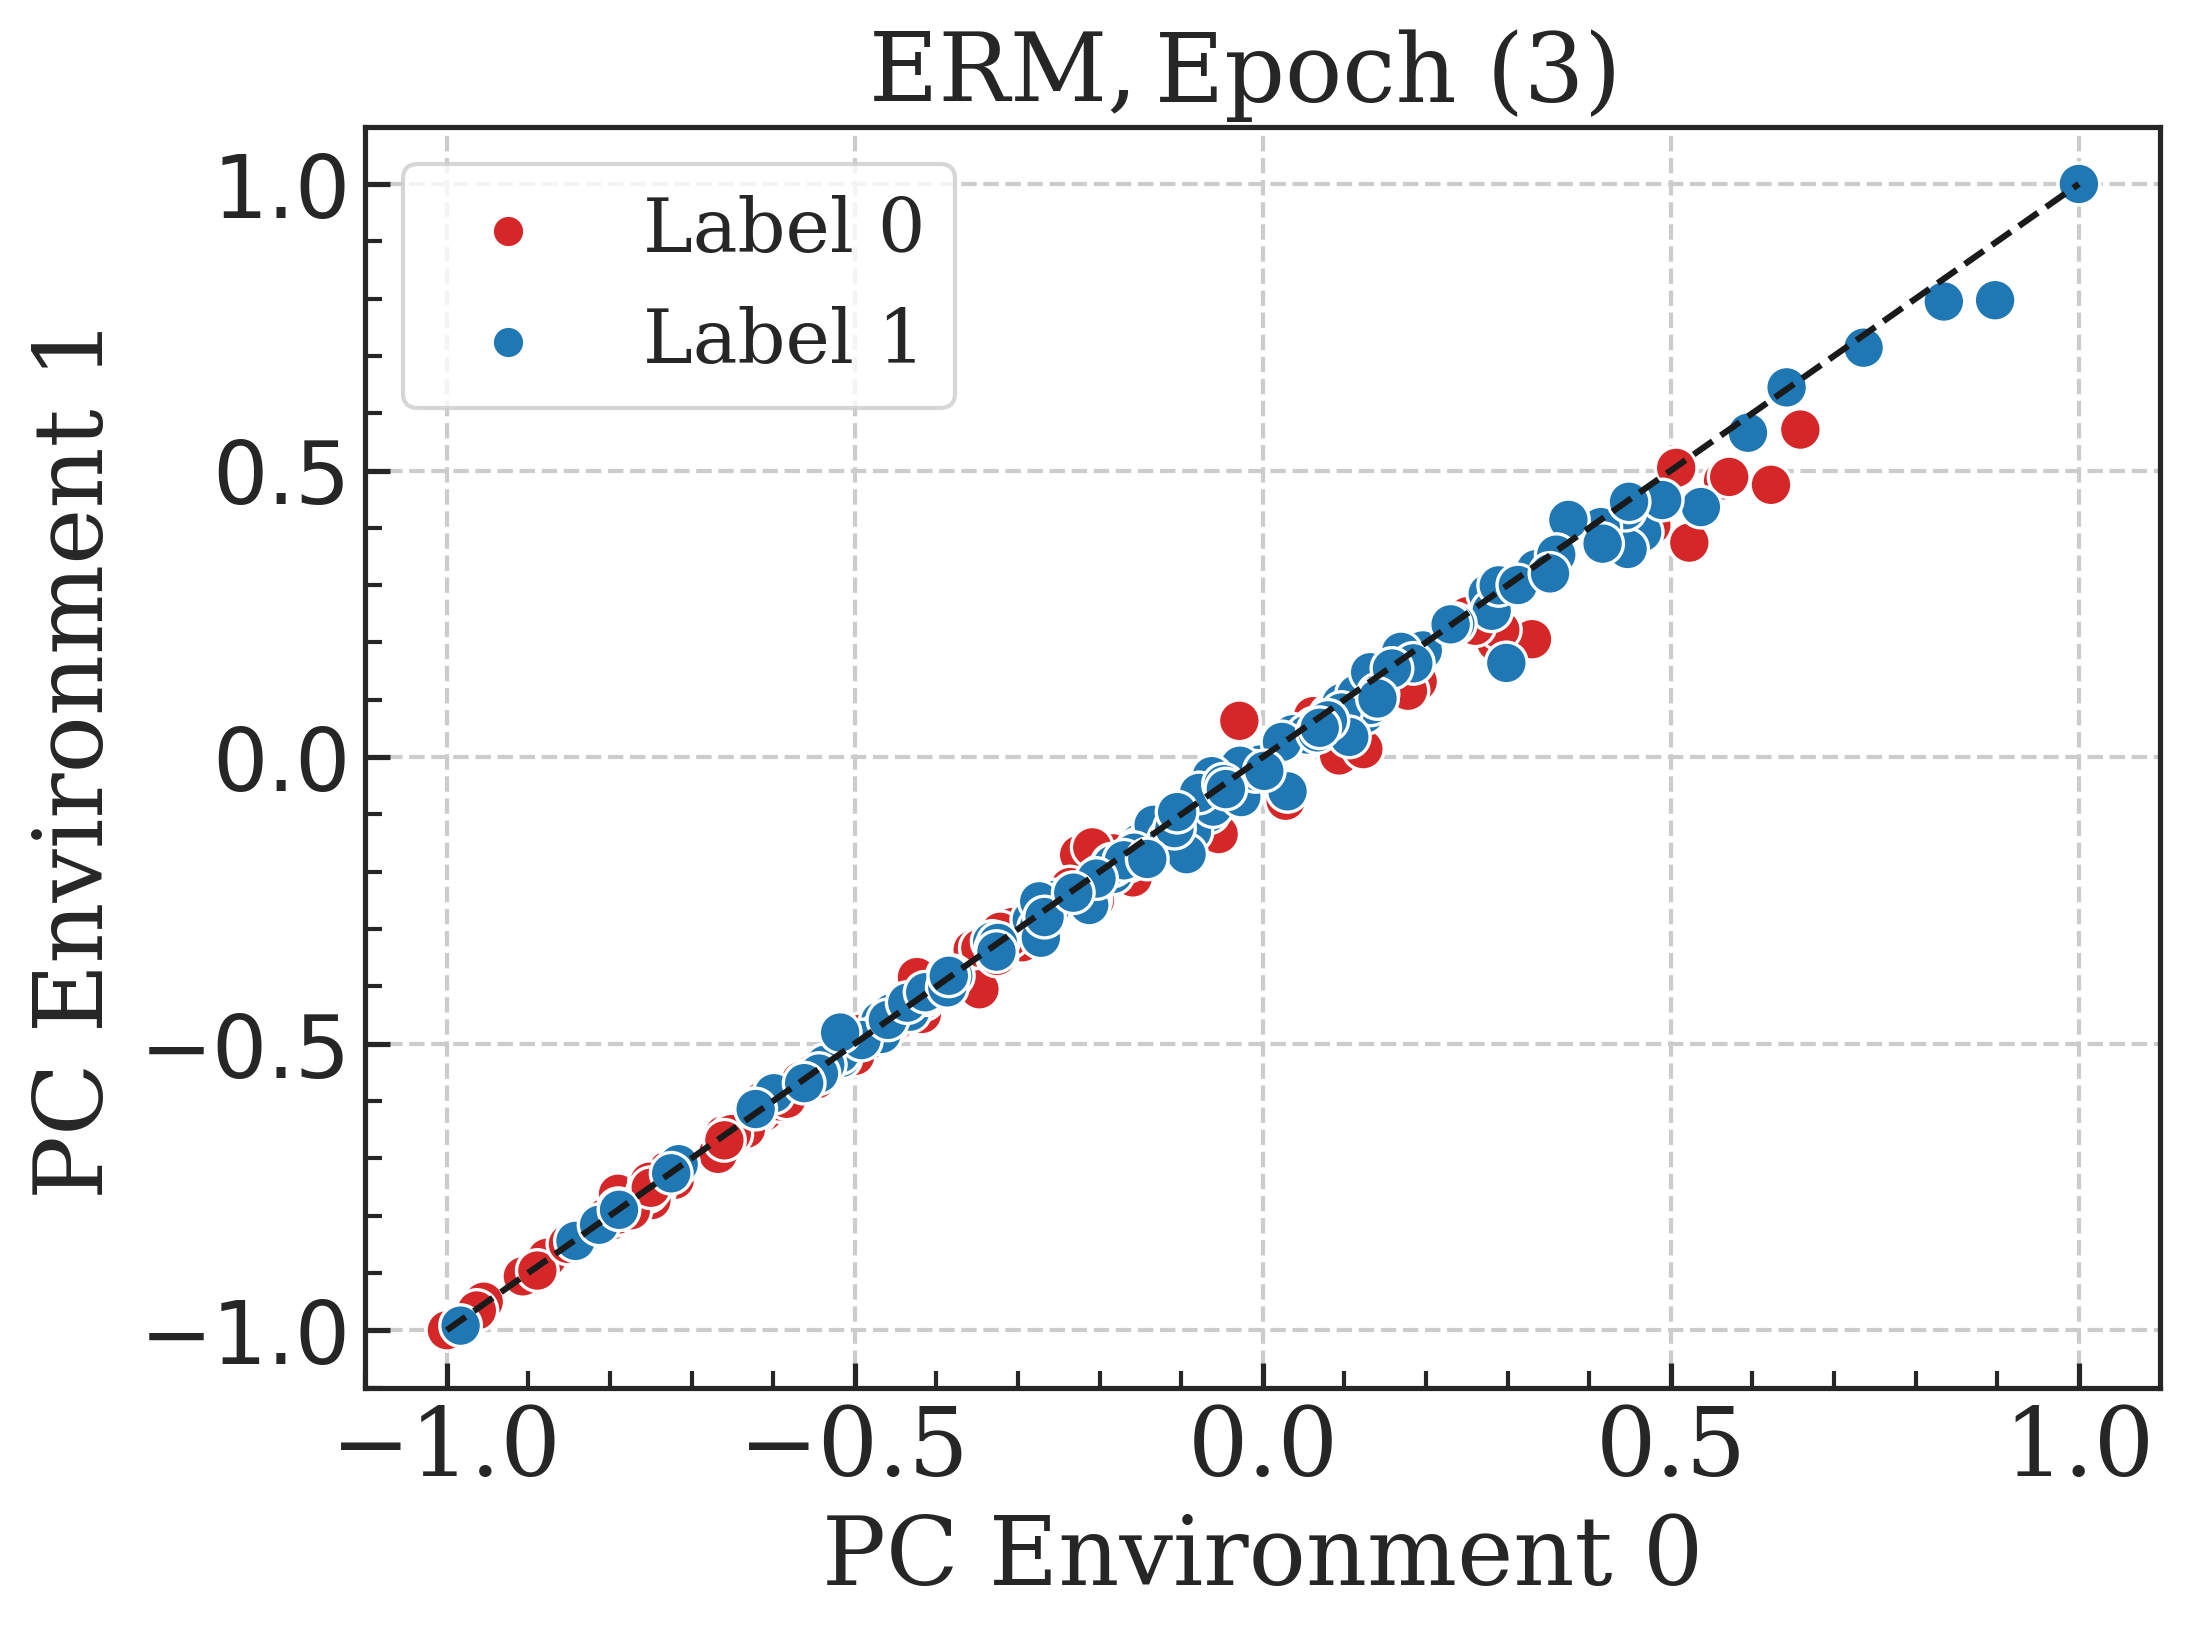
\includegraphics[width=\textwidth]{img/results_discussion/datashift/NL_5.png}
    \end{subfigure}

    \vspace{1em}

    \begin{subfigure}[b]{0.32\textwidth}
        \centering
        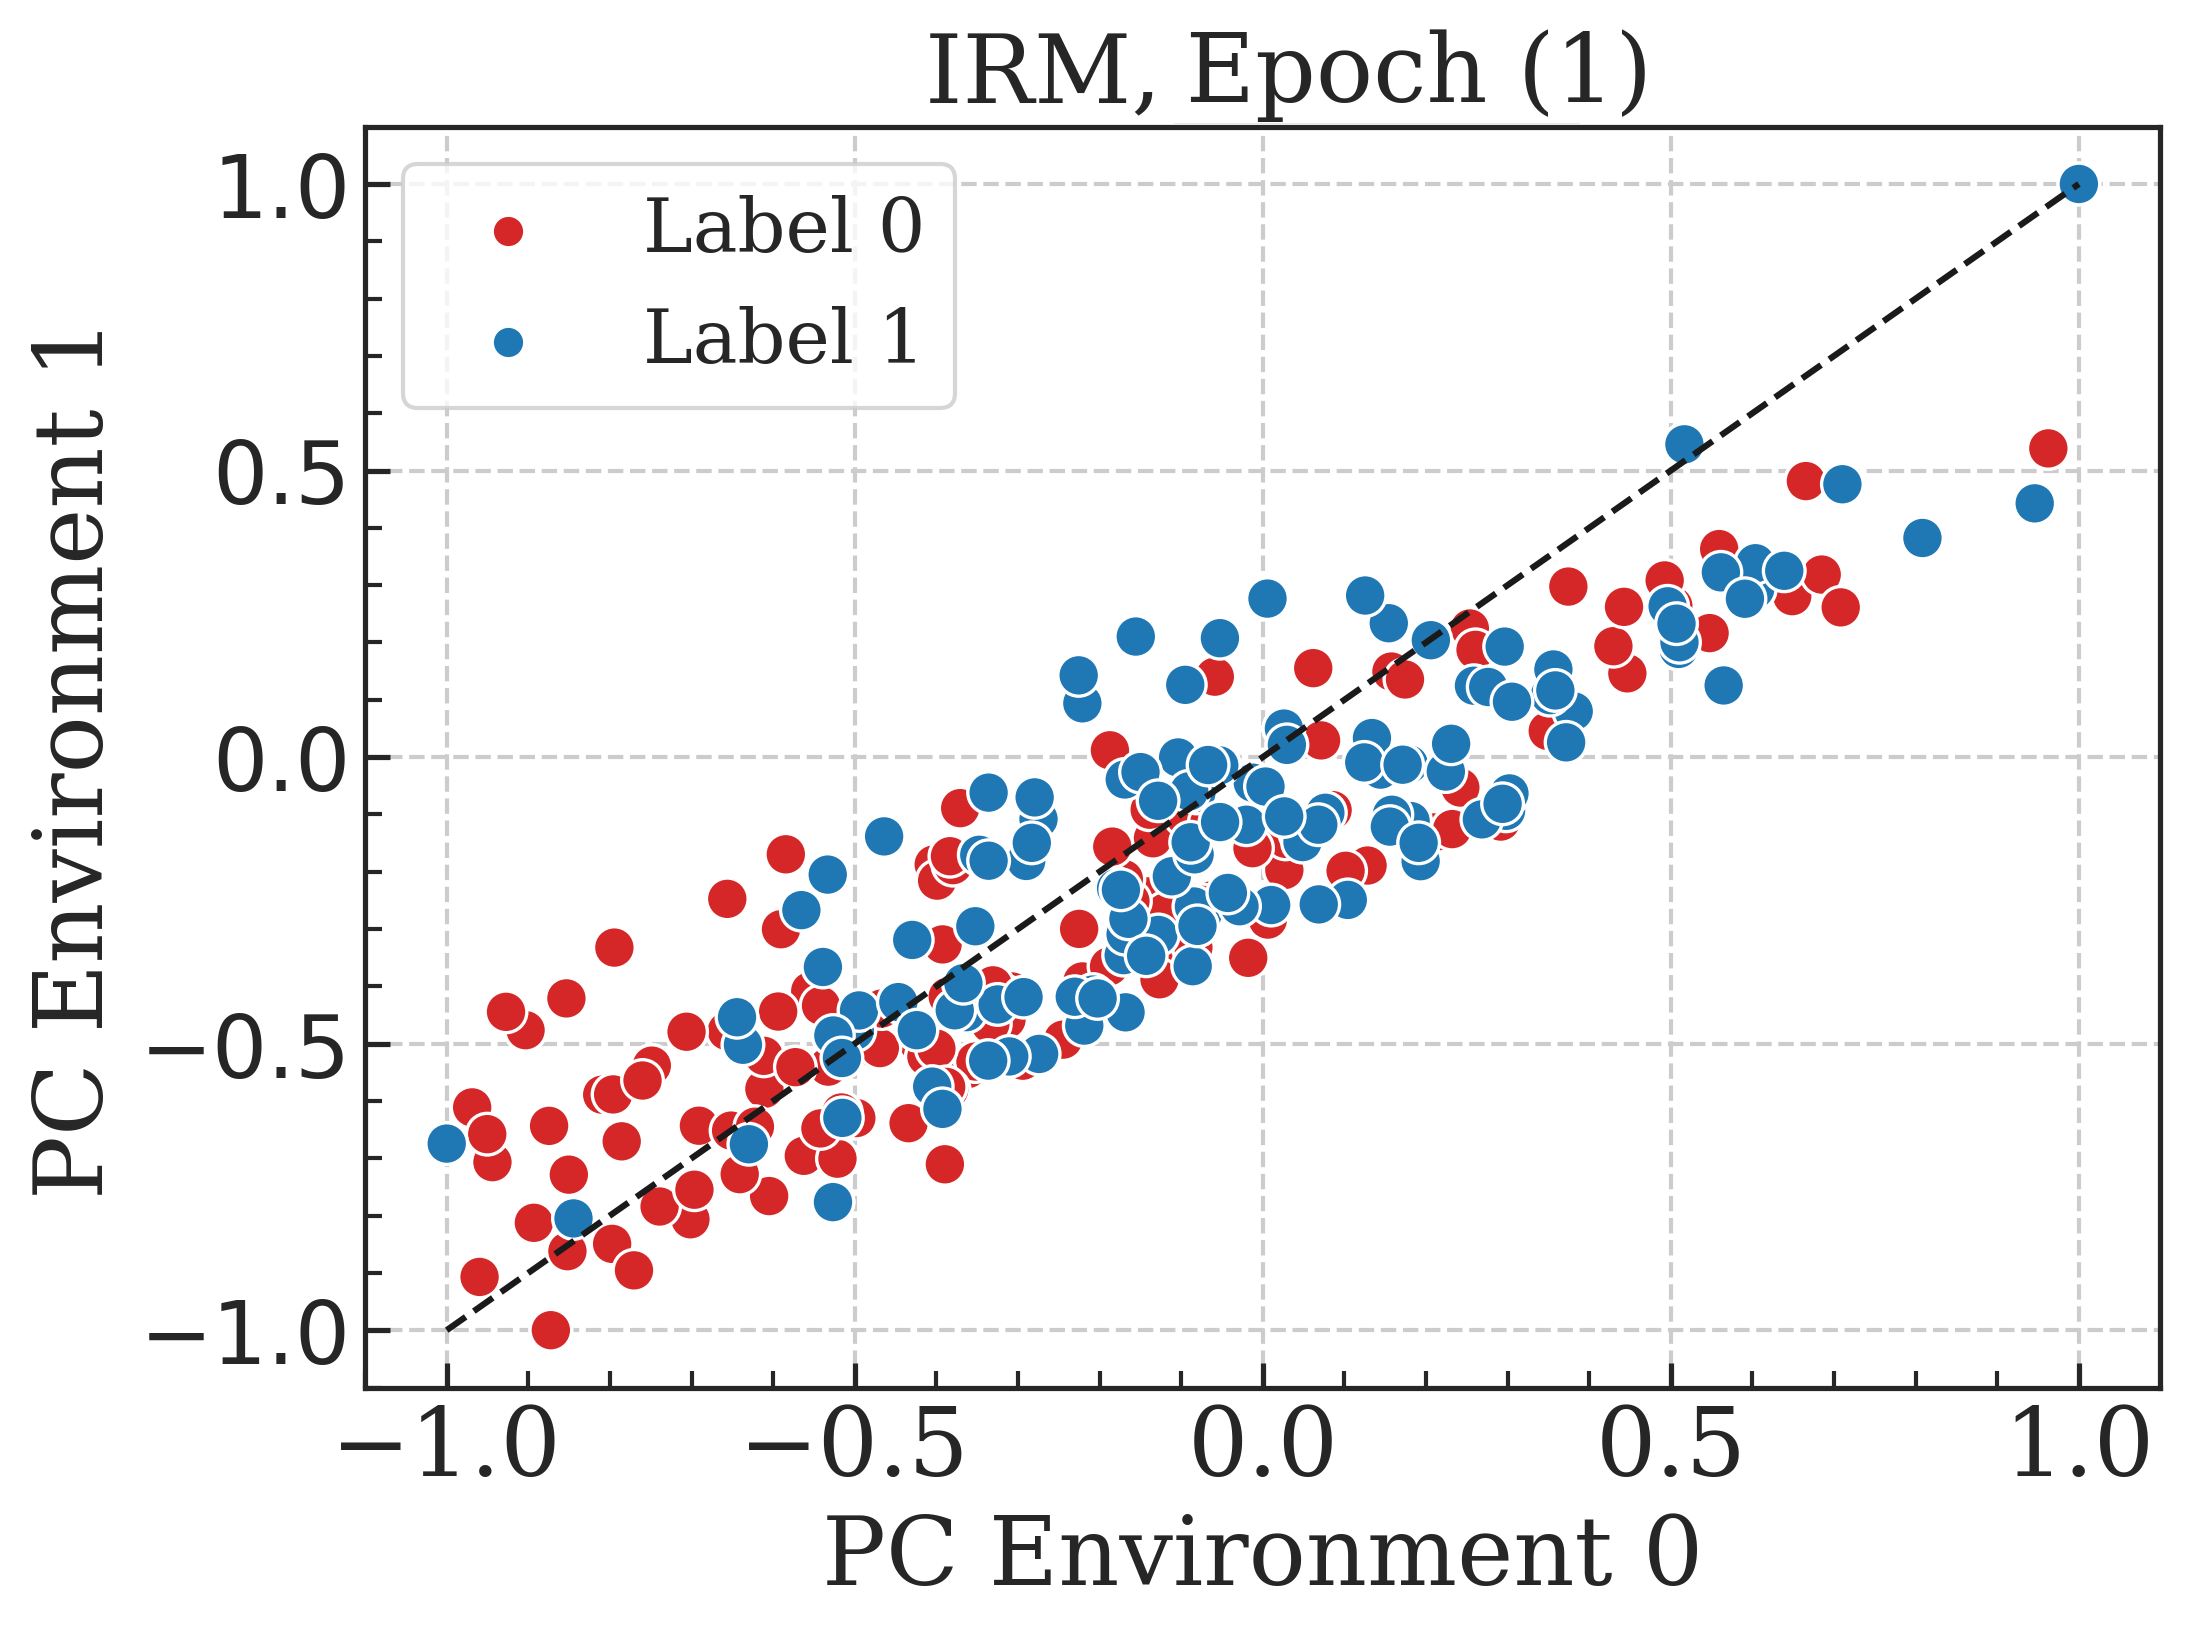
\includegraphics[width=\textwidth]{img/results_discussion/datashift/L_1.png}
    \end{subfigure}
    \hfill
    \begin{subfigure}[b]{0.32\textwidth}
        \centering
        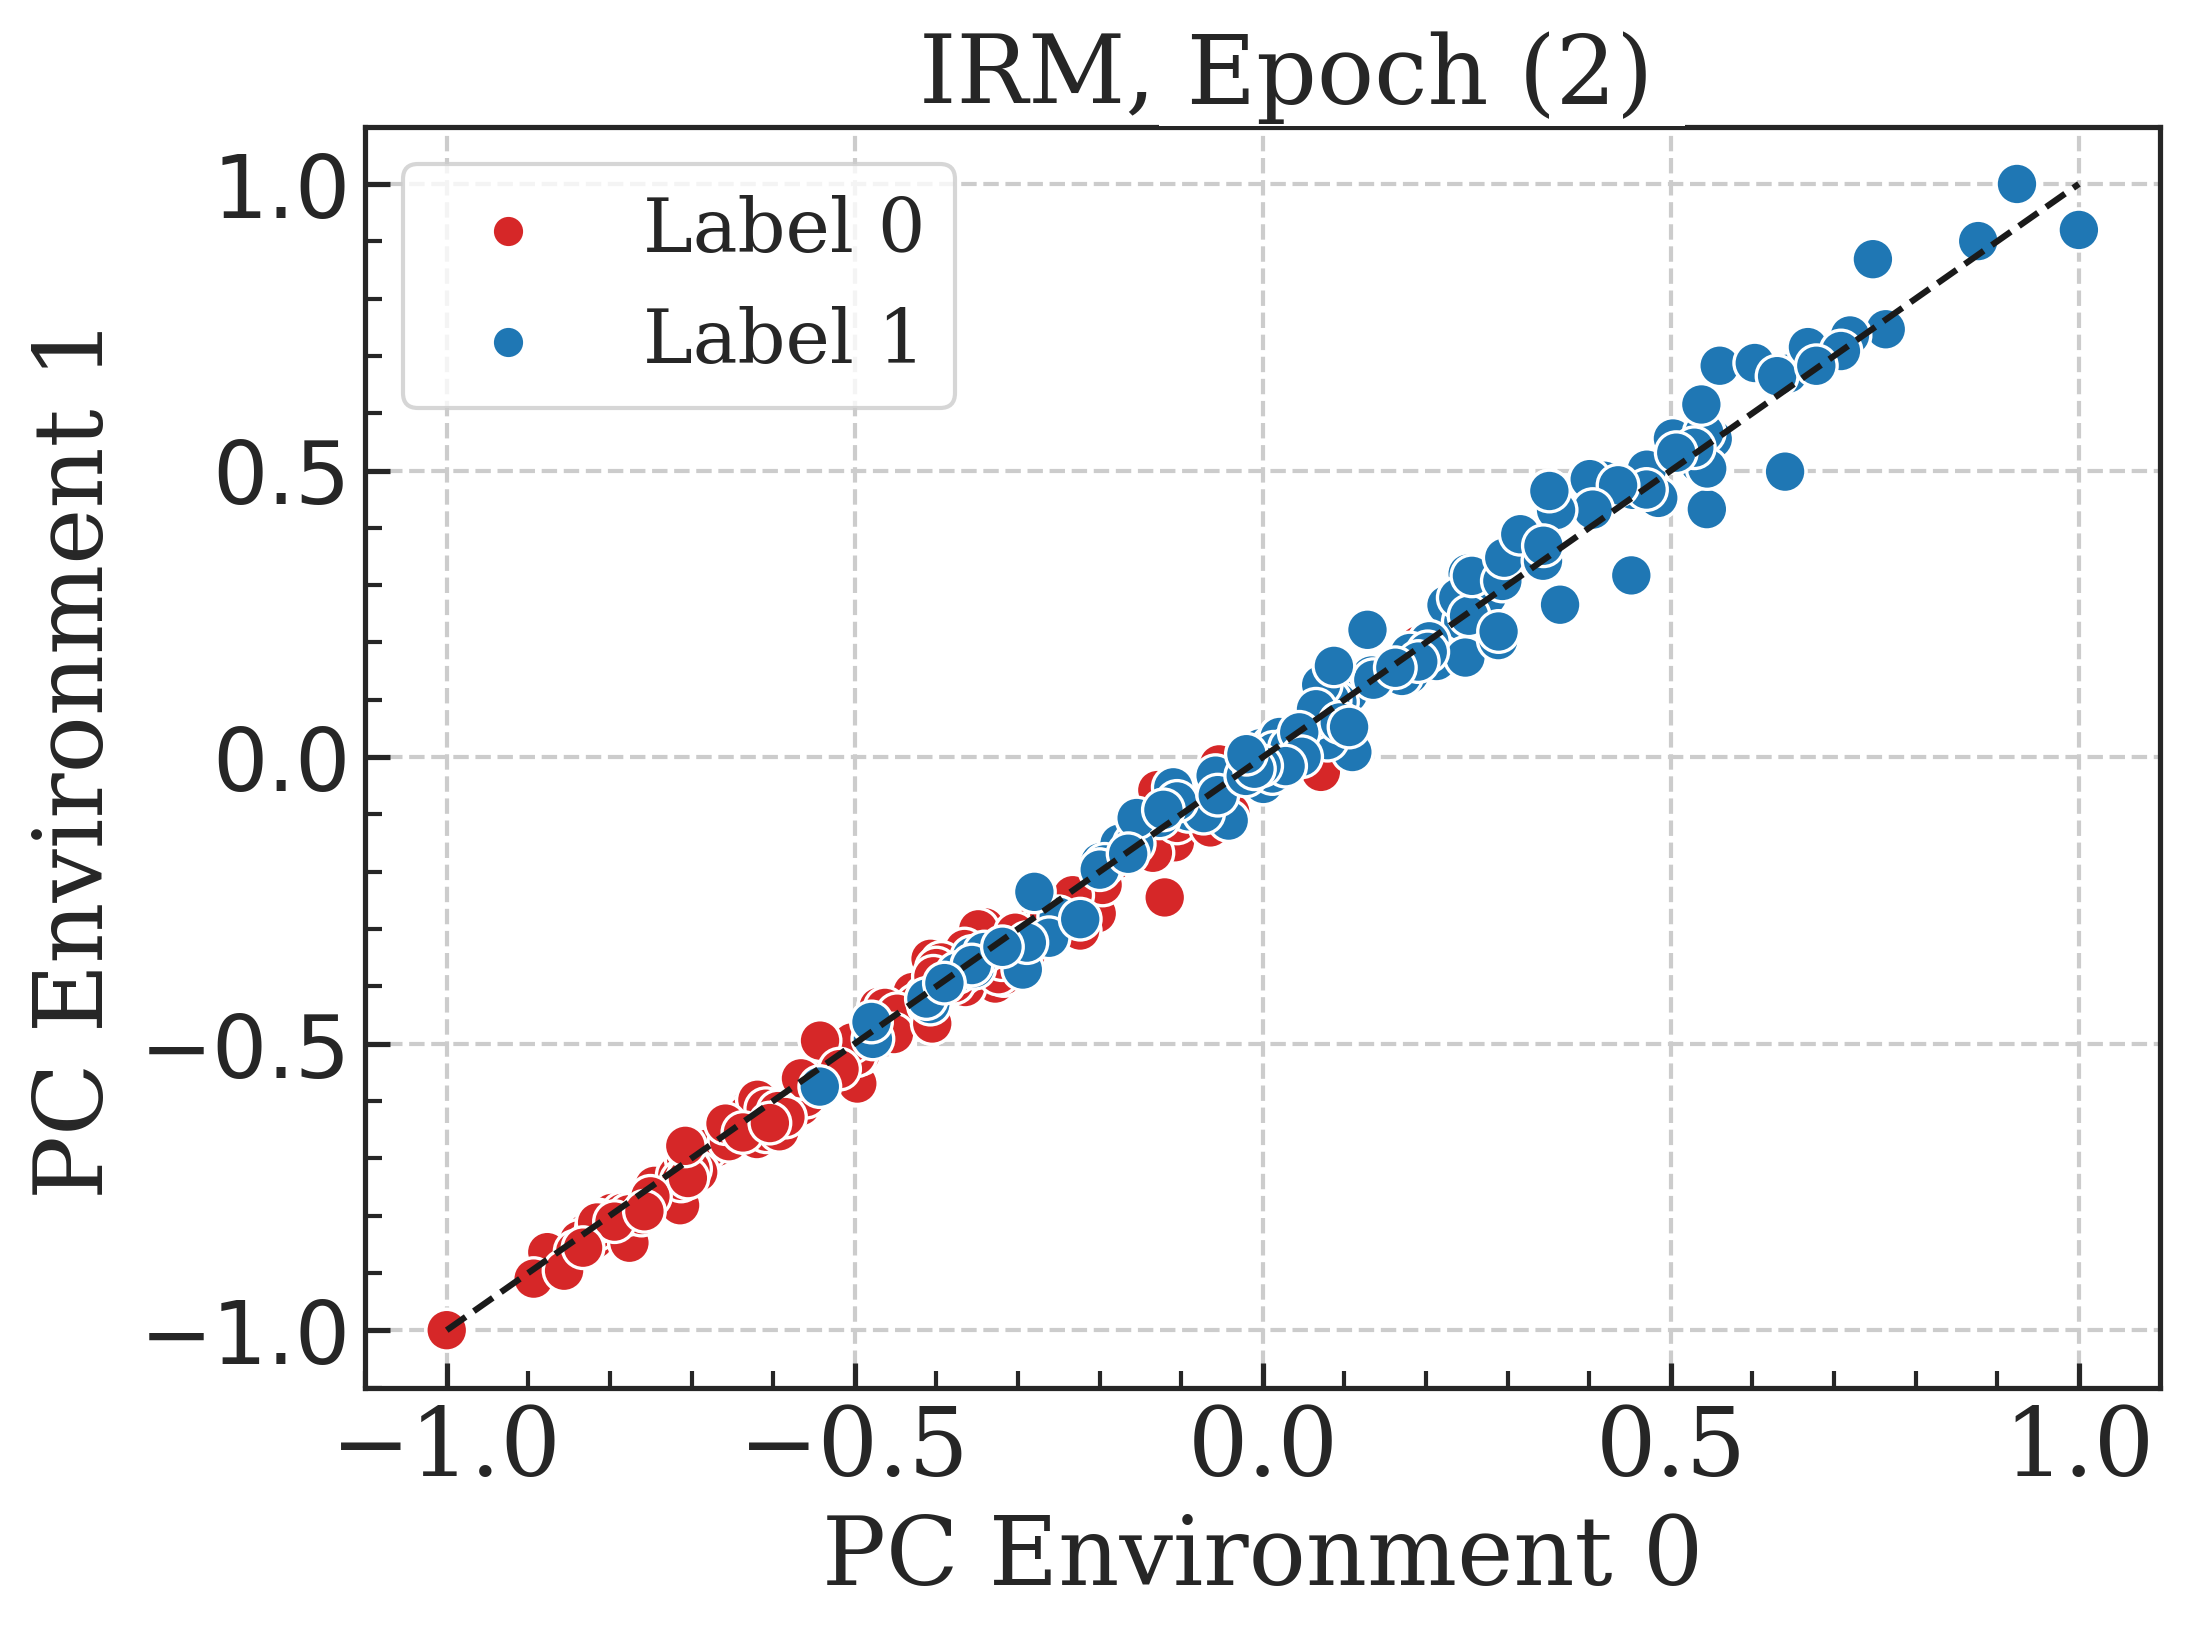
\includegraphics[width=\textwidth]{img/results_discussion/datashift/L_2.png}
    \end{subfigure}
    \hfill
    \begin{subfigure}[b]{0.32\textwidth}
        \centering
        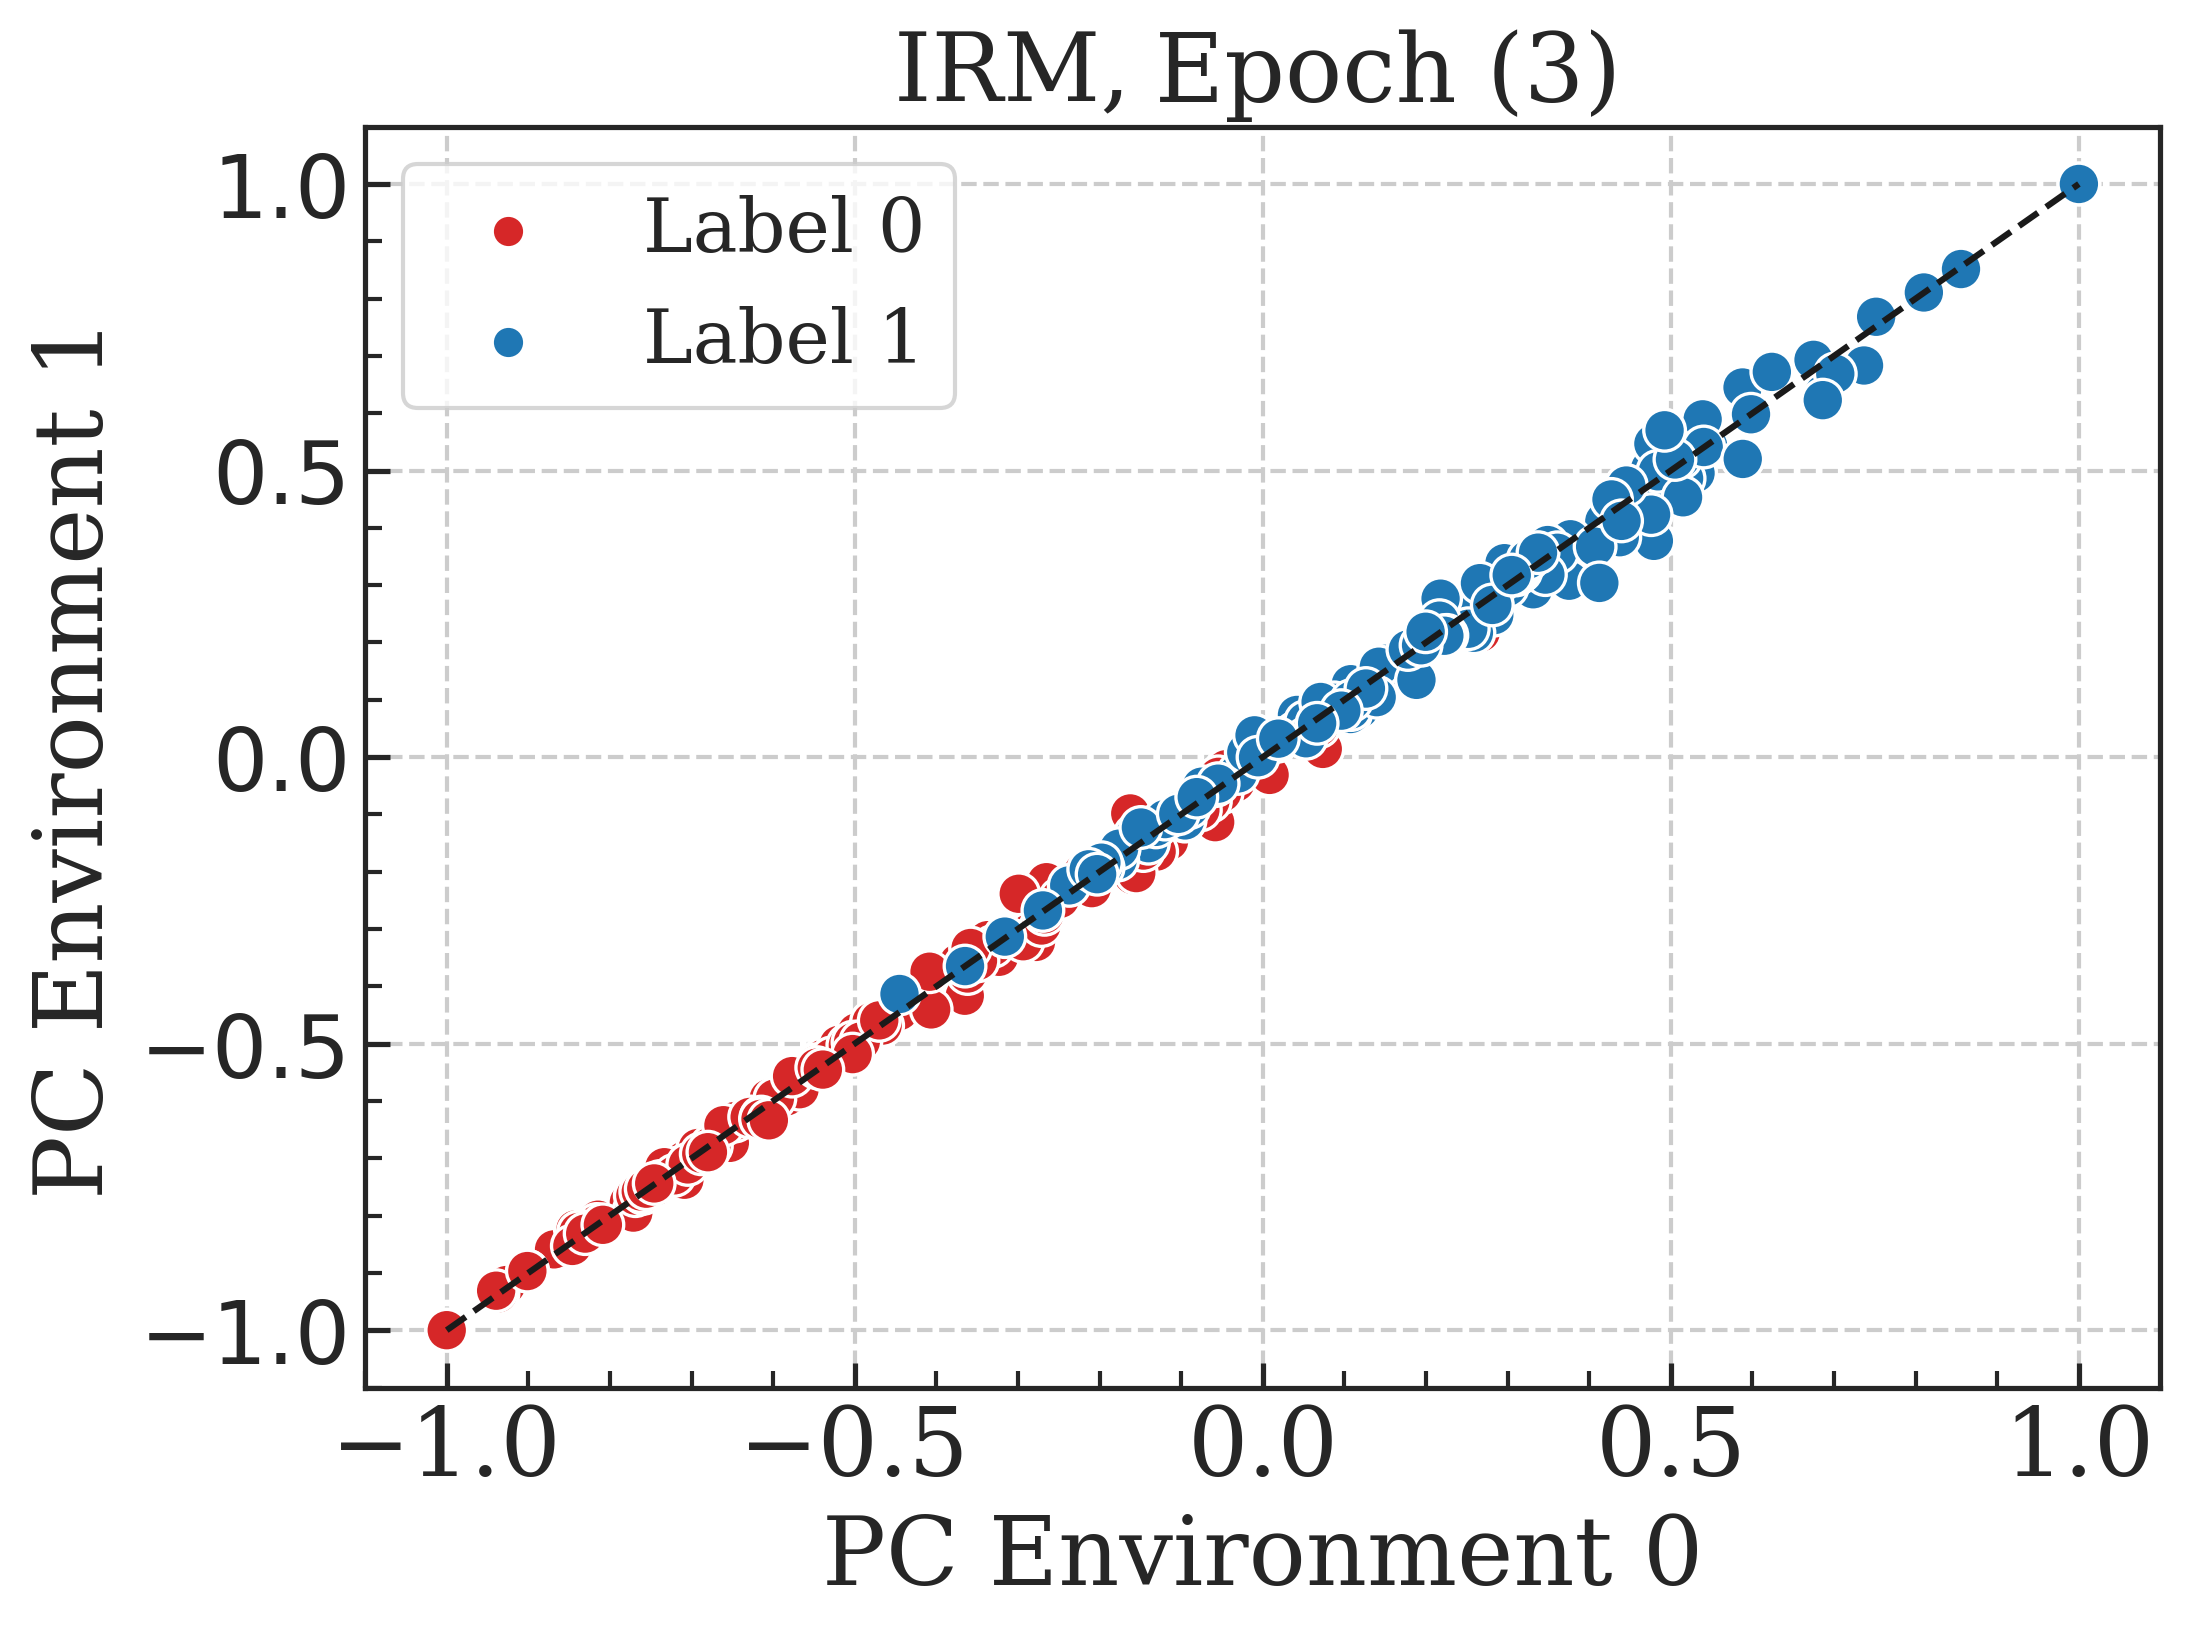
\includegraphics[width=\textwidth]{img/results_discussion/datashift/L_5.png}
    \end{subfigure}

    \caption{
    Normalized $\bm{z}_0$ vs $\bm{z}_1$ plot for ERM (top) and IRM (bottom) algorithms at three different
    training stages. Projections are colored by class membership, and the dashed line illustrates the 
    $\bm{z}_0 = \bm{z}_1$ case. Under this configuration, ERM projections display either a high cross-domain
    error or a high class-conditional variance. In contrast, IRM is able to encode a representation
    that reduces both measures at the same time, thus indicating a more robust inductive bias.
    }
    \label{fig:PCA_shift}
\end{figure}

   
Figure \ref{fig:PCA_shift} illustrates the principal component projections of the feature space representations
of samples $\bm{x}_0^{\text{sub}}$, $\bm{x}_1^{\text{sub}}$ for ERM and IRM algorithms at three 
different training stages. These results show that ERM is unable to encode a representation that is both discriminative and invariant
to domain shifts, as it either displays a high cross-domain error or a high class-conditional variance.
This indicates that its inductive bias is exclusively driven by domain-specific features or by class-specific 
features, and possibly the high learning rate avoids the model to converge to a more robust solution. 
In contrast, IRM is able to encode a representation that reduces both qualitative measures at the same time,
which indicates that the inductive bias is able to capture the most predictive features for the task at hand
without being significantly influenced by the shift in the hue factor. \\  

These measures have been shown to qualitatively
assess the suitability of the inductive bias for the aforementioned sources of randomness separately.
For that reason, they will be monitored and used in the model selection setting to assist 
in the hyperparameter tuning process and to provide a more comprehensive interpretation
of the source of robust or unrobust behavior reported by PA. \\

% As shown in Figure \ref{fig:datashift_selection}, PA-based model selection behaves differently in robust
% and non-robust algorithms. Following the reasoning derived in previous sections, it is likely that the PA
% assessment on ERM is mostly driven by standard generalization error, due to the fact that ERM is agnostic
% of the environment to which each sample belongs to and therefore to the accountable source of randomness represented
% by the environment shift. The risk minimization problem under these conditions should give rise to less informative
% predictive outcomes, given that the domain-invariant features associated with the task are less accessible, and
% thus reduce the penalization weight of mismatching samples. This intuition is supported by the fact that ERM
% optimization yields models that performs worse in all test datasets than the ones obtained through IRM,
% as can be seen in Figure \ref{fig:datashift_eval_pa}. Besides, results show that the selected model for ERM 
% performs better an all metrics for the first test environment, which contains
% the same factor configuration as one of the validation environments, and maintains or slightly decreases its performance
% for increasing levels of shift. In addition, the PA-selected model appears to encode a slight variation of the 
% decision rule from that of the accuracy-selected model, given that samples near to the decision boundary are now
% more likely classified as nines than fours, which increases specificity as much as it decreases sensitivity. \\

% Regarding PA-based model selection in robust learners, we observe the opposite behavior. Since models are more likely
% to represent domain-invariant features, each with its distinctive strategy, predictive outcomes are expected to
% be more informative and thus increase the penalization contribution of mismatching samples, which will be the ones
% containing domain-invariant features that are not sufficiently considered in the inductive bias of the model. PA
% model selection under these conditions is thus more likely to favor sets of weights that perform better under
% increasing levels of shift, at the expense of losing predictive power on the environments in which it operated. 
% Results align with this interpretation, as we observe a notable increase in performance across all shifted datasets
% with respect to the accuracy-selected model, especially in the LISA case, at the expense of significantly decreasing
% performance on the first environment.\\


% \begin{figure}[H]
%     \centering
%     \begin{subfigure}[b]{0.6\textwidth}
%         \centering
%         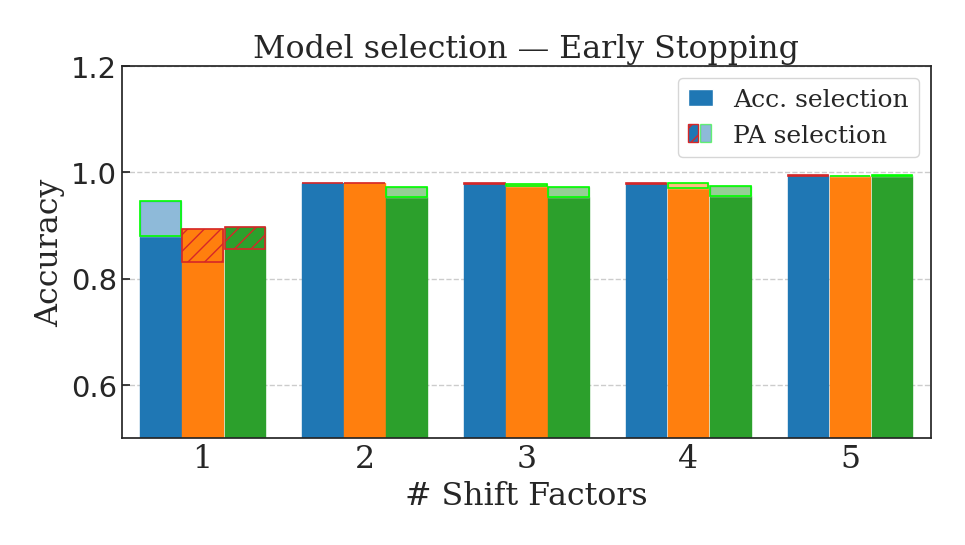
\includegraphics[width=\textwidth]{img/results_discussion/datashift/paper_selection_ppred=1.0_met=acc.png}
%     \end{subfigure}

%     \begin{subfigure}[b]{0.6\textwidth}
%         \centering
%         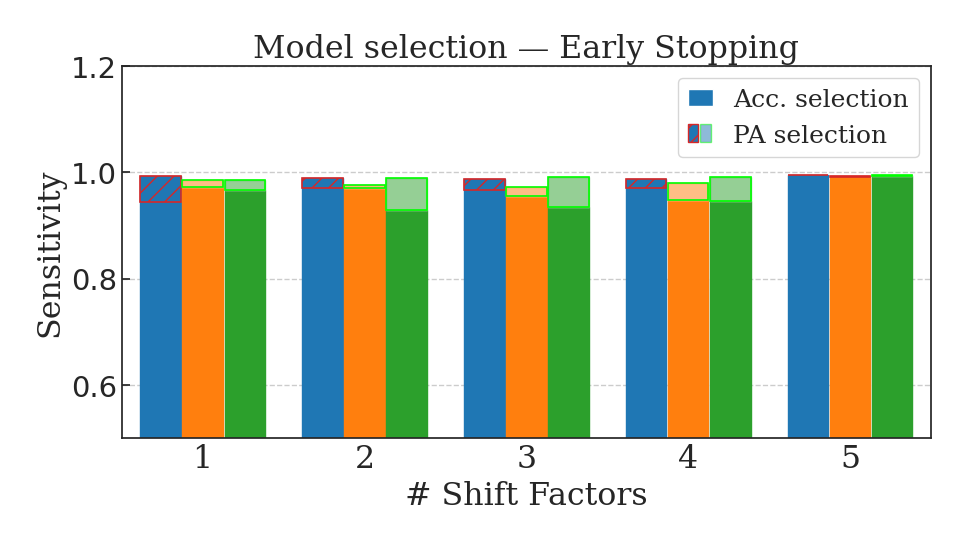
\includegraphics[width=\textwidth]{img/results_discussion/datashift/paper_selection_ppred=1.0_met=sensitivity.png}
%     \end{subfigure}

%     \begin{subfigure}[b]{0.6\textwidth}
%         \centering
%         \includegraphics[width=\textwidth]{img/results_discussion/datashift/paper_selection_ppred=1.0_met=specificity.png}
%     \end{subfigure}
%     \caption{
%     Accuracy, sensitivity and precision displayed by sets of ResNet18 weights on
%     shifted test datasets, obtained through ERM, IRM and LISA
%     training procedures. Accuracy-based selection is compared to PA-based selection, both
%     operating with a validation dataset composed of samples of environments 0 and 1.
%     }
%     \label{fig:datashift_selection}
% \end{figure}



% Model:  0
% Accuracy:  [88.08000088 97.94499874 98.05499911 97.94499874 99.44000244]
% PA_diff:  [ 6.52999878e+00 -5.00082970e-03 -3.19999456e-01 -1.19996071e-01
%  -7.50005245e-02]
% Model:  1
% Accuracy:  [89.34500217 98.00500274 97.43499756 97.11999893 99.36000109]
% PA_diff:  [-6.13500476  0.          0.41000247  0.88000298  0.01499653]
% Model:  2
% Accuracy:  [89.74499702 95.35499811 95.3700006  95.59500217 99.32000041]
% PA_diff:  [-4.24499512  1.85500383  1.87000036  1.78999901  0.06999969]



% \begin{table}[H]
%     \centering
%     \resizebox{\textwidth}{!}{%
%     \begin{tabular}{l|cl|cl|cl|cl|cl|cl}
%     \multirow{2}{*}{} & \multicolumn{2}{c|}{\textbf{0}} & \multicolumn{2}{c|}{\textbf{1}} & \multicolumn{2}{c|}{\textbf{2}} & \multicolumn{2}{c|}{\textbf{3}} & \multicolumn{2}{c|}{\textbf{4}} & \multicolumn{2}{c}{\textbf{5}} \\
%     \textbf{{\color{tab:blue} \textbf{ERM}}} & Acc. & $\Delta_{\operatorname{PA}}$ & Acc. & $\Delta_{\operatorname{PA}}$ & Acc. & $\Delta_{\operatorname{PA}}$ & Acc. & $\Delta_{\operatorname{PA}}$ & Acc. & $\Delta_{\operatorname{PA}}$ & Acc. & $\Delta_{\operatorname{PA}}$ \\
%     \midrule
%     Specificity & 99.4 & \PlusMinus 0.01 & 68.0 & {\color{tab:green}  \textbf{\Plus 10.1}} & 45.2 & {\color{tab:red} \textbf{\Minus 10.1}} & 42.1 & {\color{tab:red} \textbf{\Minus 6.0}} & 42.9 & {\color{tab:red} \textbf{\Minus 9.3}} & 32.0 & {\color{tab:red} \textbf{\Minus 3.8}} \\
%     Sensitivity & \textbf{99.4} & \PlusMinus 0.01 & 67.1 & {\color{tab:red} \textbf{\Minus 7.9}} & 44.9 & {\color{tab:green}  \textbf{\Plus 0.8}} & 42.7 & {\color{tab:green}  \textbf{\Plus 1.3}} & 39.1 & {\color{tab:green}  \textbf{\Plus 1.5}} & 30.3 & {\color{tab:green}  \textbf{\Plus 1.4}} \\
%     \midrule
%     Accuracy & 88.1 & \PlusMinus 0.01 & 97.9 & \PlusMinus 0.01 & 98.1 & \PlusMinus 0.01 & 97.9 & \PlusMinus 0.01 & 42.5 & \PlusMinus 0.01 & 32.8 & \PlusMinus 0.01 \\
%     \midrule
%     \addlinespace
%     \addlinespace
%     \textbf{{\color{tab:orange} \textbf{IRM}}} & Acc. & $\Delta_{\operatorname{PA}}$ & Acc. & $\Delta_{\operatorname{PA}}$ & Acc. & $\Delta_{\operatorname{PA}}$ & Acc. & $\Delta_{\operatorname{PA}}$ & Acc. & $\Delta_{\operatorname{PA}}$ & Acc. & $\Delta_{\operatorname{PA}}$ \\
%     \midrule
%     Specificity & 99.4 & \PlusMinus 0.01 & 68.0 & {\color{tab:green}  \textbf{\Plus 10.1}} & 45.2 & {\color{tab:red} \textbf{\Minus 10.1}} & 42.1 & {\color{tab:red} \textbf{\Minus 6.0}} & 42.9 & {\color{tab:red} \textbf{\Minus 9.3}} & 32.0 & {\color{tab:red} \textbf{\Minus 3.8}} \\
%     Sensitivity & \textbf{99.4} & \PlusMinus 0.01 & 67.1 & {\color{tab:red} \textbf{\Minus 7.9}} & 44.9 & {\color{tab:green}  \textbf{\Plus 0.8}} & 42.7 & {\color{tab:green}  \textbf{\Plus 1.3}} & 39.1 & {\color{tab:green}  \textbf{\Plus 1.5}} & 30.3 & {\color{tab:green}  \textbf{\Plus 1.4}} \\
%     \midrule
%     Accuracy & 99.4 & \PlusMinus 0.01 & 59.3 & \PlusMinus 0.01 & 46.7 & \PlusMinus 0.01 & 44.9 & \PlusMinus 0.01 & 42.5 & \PlusMinus 0.01 & 32.8 & \PlusMinus 0.01 \\
%     \midrule
%     \addlinespace
%     \addlinespace
%     \textbf{{\color{tab:green} \textbf{LISA}}} & Acc. & $\Delta_{\operatorname{PA}}$ & Acc. & $\Delta_{\operatorname{PA}}$ & Acc. & $\Delta_{\operatorname{PA}}$ & Acc. & $\Delta_{\operatorname{PA}}$ & Acc. & $\Delta_{\operatorname{PA}}$ & Acc. & $\Delta_{\operatorname{PA}}$ \\
%     \midrule
%     Specificity & 99.4 & \PlusMinus 0.01 & 68.0 & {\color{tab:green}  \textbf{\Plus 10.1}} & 45.2 & {\color{tab:red} \textbf{\Minus 10.1}} & 42.1 & {\color{tab:red} \textbf{\Minus 6.0}} & 42.9 & {\color{tab:red} \textbf{\Minus 9.3}} & 32.0 & {\color{tab:red} \textbf{\Minus 3.8}} \\
%     Sensitivity & \textbf{99.4} & \PlusMinus 0.01 & 67.1 & {\color{tab:red} \textbf{\Minus 7.9}} & 44.9 & {\color{tab:green}  \textbf{\Plus 0.8}} & 42.7 & {\color{tab:green}  \textbf{\Plus 1.3}} & 39.1 & {\color{tab:green}  \textbf{\Plus 1.5}} & 30.3 & {\color{tab:green}  \textbf{\Plus 1.4}} \\
%     \midrule
%     Accuracy & 99.4 & \PlusMinus 0.01 & 59.3 & \PlusMinus 0.01 & 46.7 & \PlusMinus 0.01 & 44.9 & \PlusMinus 0.01 & 42.5 & \PlusMinus 0.01 & 32.8 & \PlusMinus 0.01 \\
%     \bottomrule
%     \end{tabular}%
%     }
%     \caption{REMOVEopt=adam-lr=0.0001-mf=hue-npair=FalseREMOVE Test performance on increasingly shifted datasets for models selected during ERM and IRM procedures. Different validation datasets are used, and the selection capabilities of PA and validation accuracy are compared.}
%     \label{tab:paper_msel}
%     \end{table}




\cleardoublepage
